% Options for packages loaded elsewhere
\PassOptionsToPackage{unicode}{hyperref}
\PassOptionsToPackage{hyphens}{url}
\PassOptionsToPackage{dvipsnames,svgnames,x11names}{xcolor}
%
\documentclass[
  letterpaper,
  DIV=11,
  numbers=noendperiod]{scrreprt}

\usepackage{amsmath,amssymb}
\usepackage{iftex}
\ifPDFTeX
  \usepackage[T1]{fontenc}
  \usepackage[utf8]{inputenc}
  \usepackage{textcomp} % provide euro and other symbols
\else % if luatex or xetex
  \usepackage{unicode-math}
  \defaultfontfeatures{Scale=MatchLowercase}
  \defaultfontfeatures[\rmfamily]{Ligatures=TeX,Scale=1}
\fi
\usepackage{lmodern}
\ifPDFTeX\else  
    % xetex/luatex font selection
\fi
% Use upquote if available, for straight quotes in verbatim environments
\IfFileExists{upquote.sty}{\usepackage{upquote}}{}
\IfFileExists{microtype.sty}{% use microtype if available
  \usepackage[]{microtype}
  \UseMicrotypeSet[protrusion]{basicmath} % disable protrusion for tt fonts
}{}
\makeatletter
\@ifundefined{KOMAClassName}{% if non-KOMA class
  \IfFileExists{parskip.sty}{%
    \usepackage{parskip}
  }{% else
    \setlength{\parindent}{0pt}
    \setlength{\parskip}{6pt plus 2pt minus 1pt}}
}{% if KOMA class
  \KOMAoptions{parskip=half}}
\makeatother
\usepackage{xcolor}
\setlength{\emergencystretch}{3em} % prevent overfull lines
\setcounter{secnumdepth}{5}
% Make \paragraph and \subparagraph free-standing
\makeatletter
\ifx\paragraph\undefined\else
  \let\oldparagraph\paragraph
  \renewcommand{\paragraph}{
    \@ifstar
      \xxxParagraphStar
      \xxxParagraphNoStar
  }
  \newcommand{\xxxParagraphStar}[1]{\oldparagraph*{#1}\mbox{}}
  \newcommand{\xxxParagraphNoStar}[1]{\oldparagraph{#1}\mbox{}}
\fi
\ifx\subparagraph\undefined\else
  \let\oldsubparagraph\subparagraph
  \renewcommand{\subparagraph}{
    \@ifstar
      \xxxSubParagraphStar
      \xxxSubParagraphNoStar
  }
  \newcommand{\xxxSubParagraphStar}[1]{\oldsubparagraph*{#1}\mbox{}}
  \newcommand{\xxxSubParagraphNoStar}[1]{\oldsubparagraph{#1}\mbox{}}
\fi
\makeatother

\usepackage{color}
\usepackage{fancyvrb}
\newcommand{\VerbBar}{|}
\newcommand{\VERB}{\Verb[commandchars=\\\{\}]}
\DefineVerbatimEnvironment{Highlighting}{Verbatim}{commandchars=\\\{\}}
% Add ',fontsize=\small' for more characters per line
\usepackage{framed}
\definecolor{shadecolor}{RGB}{241,243,245}
\newenvironment{Shaded}{\begin{snugshade}}{\end{snugshade}}
\newcommand{\AlertTok}[1]{\textcolor[rgb]{0.68,0.00,0.00}{#1}}
\newcommand{\AnnotationTok}[1]{\textcolor[rgb]{0.37,0.37,0.37}{#1}}
\newcommand{\AttributeTok}[1]{\textcolor[rgb]{0.40,0.45,0.13}{#1}}
\newcommand{\BaseNTok}[1]{\textcolor[rgb]{0.68,0.00,0.00}{#1}}
\newcommand{\BuiltInTok}[1]{\textcolor[rgb]{0.00,0.23,0.31}{#1}}
\newcommand{\CharTok}[1]{\textcolor[rgb]{0.13,0.47,0.30}{#1}}
\newcommand{\CommentTok}[1]{\textcolor[rgb]{0.37,0.37,0.37}{#1}}
\newcommand{\CommentVarTok}[1]{\textcolor[rgb]{0.37,0.37,0.37}{\textit{#1}}}
\newcommand{\ConstantTok}[1]{\textcolor[rgb]{0.56,0.35,0.01}{#1}}
\newcommand{\ControlFlowTok}[1]{\textcolor[rgb]{0.00,0.23,0.31}{\textbf{#1}}}
\newcommand{\DataTypeTok}[1]{\textcolor[rgb]{0.68,0.00,0.00}{#1}}
\newcommand{\DecValTok}[1]{\textcolor[rgb]{0.68,0.00,0.00}{#1}}
\newcommand{\DocumentationTok}[1]{\textcolor[rgb]{0.37,0.37,0.37}{\textit{#1}}}
\newcommand{\ErrorTok}[1]{\textcolor[rgb]{0.68,0.00,0.00}{#1}}
\newcommand{\ExtensionTok}[1]{\textcolor[rgb]{0.00,0.23,0.31}{#1}}
\newcommand{\FloatTok}[1]{\textcolor[rgb]{0.68,0.00,0.00}{#1}}
\newcommand{\FunctionTok}[1]{\textcolor[rgb]{0.28,0.35,0.67}{#1}}
\newcommand{\ImportTok}[1]{\textcolor[rgb]{0.00,0.46,0.62}{#1}}
\newcommand{\InformationTok}[1]{\textcolor[rgb]{0.37,0.37,0.37}{#1}}
\newcommand{\KeywordTok}[1]{\textcolor[rgb]{0.00,0.23,0.31}{\textbf{#1}}}
\newcommand{\NormalTok}[1]{\textcolor[rgb]{0.00,0.23,0.31}{#1}}
\newcommand{\OperatorTok}[1]{\textcolor[rgb]{0.37,0.37,0.37}{#1}}
\newcommand{\OtherTok}[1]{\textcolor[rgb]{0.00,0.23,0.31}{#1}}
\newcommand{\PreprocessorTok}[1]{\textcolor[rgb]{0.68,0.00,0.00}{#1}}
\newcommand{\RegionMarkerTok}[1]{\textcolor[rgb]{0.00,0.23,0.31}{#1}}
\newcommand{\SpecialCharTok}[1]{\textcolor[rgb]{0.37,0.37,0.37}{#1}}
\newcommand{\SpecialStringTok}[1]{\textcolor[rgb]{0.13,0.47,0.30}{#1}}
\newcommand{\StringTok}[1]{\textcolor[rgb]{0.13,0.47,0.30}{#1}}
\newcommand{\VariableTok}[1]{\textcolor[rgb]{0.07,0.07,0.07}{#1}}
\newcommand{\VerbatimStringTok}[1]{\textcolor[rgb]{0.13,0.47,0.30}{#1}}
\newcommand{\WarningTok}[1]{\textcolor[rgb]{0.37,0.37,0.37}{\textit{#1}}}

\providecommand{\tightlist}{%
  \setlength{\itemsep}{0pt}\setlength{\parskip}{0pt}}\usepackage{longtable,booktabs,array}
\usepackage{calc} % for calculating minipage widths
% Correct order of tables after \paragraph or \subparagraph
\usepackage{etoolbox}
\makeatletter
\patchcmd\longtable{\par}{\if@noskipsec\mbox{}\fi\par}{}{}
\makeatother
% Allow footnotes in longtable head/foot
\IfFileExists{footnotehyper.sty}{\usepackage{footnotehyper}}{\usepackage{footnote}}
\makesavenoteenv{longtable}
\usepackage{graphicx}
\makeatletter
\newsavebox\pandoc@box
\newcommand*\pandocbounded[1]{% scales image to fit in text height/width
  \sbox\pandoc@box{#1}%
  \Gscale@div\@tempa{\textheight}{\dimexpr\ht\pandoc@box+\dp\pandoc@box\relax}%
  \Gscale@div\@tempb{\linewidth}{\wd\pandoc@box}%
  \ifdim\@tempb\p@<\@tempa\p@\let\@tempa\@tempb\fi% select the smaller of both
  \ifdim\@tempa\p@<\p@\scalebox{\@tempa}{\usebox\pandoc@box}%
  \else\usebox{\pandoc@box}%
  \fi%
}
% Set default figure placement to htbp
\def\fps@figure{htbp}
\makeatother
% definitions for citeproc citations
\NewDocumentCommand\citeproctext{}{}
\NewDocumentCommand\citeproc{mm}{%
  \begingroup\def\citeproctext{#2}\cite{#1}\endgroup}
\makeatletter
 % allow citations to break across lines
 \let\@cite@ofmt\@firstofone
 % avoid brackets around text for \cite:
 \def\@biblabel#1{}
 \def\@cite#1#2{{#1\if@tempswa , #2\fi}}
\makeatother
\newlength{\cslhangindent}
\setlength{\cslhangindent}{1.5em}
\newlength{\csllabelwidth}
\setlength{\csllabelwidth}{3em}
\newenvironment{CSLReferences}[2] % #1 hanging-indent, #2 entry-spacing
 {\begin{list}{}{%
  \setlength{\itemindent}{0pt}
  \setlength{\leftmargin}{0pt}
  \setlength{\parsep}{0pt}
  % turn on hanging indent if param 1 is 1
  \ifodd #1
   \setlength{\leftmargin}{\cslhangindent}
   \setlength{\itemindent}{-1\cslhangindent}
  \fi
  % set entry spacing
  \setlength{\itemsep}{#2\baselineskip}}}
 {\end{list}}
\usepackage{calc}
\newcommand{\CSLBlock}[1]{\hfill\break\parbox[t]{\linewidth}{\strut\ignorespaces#1\strut}}
\newcommand{\CSLLeftMargin}[1]{\parbox[t]{\csllabelwidth}{\strut#1\strut}}
\newcommand{\CSLRightInline}[1]{\parbox[t]{\linewidth - \csllabelwidth}{\strut#1\strut}}
\newcommand{\CSLIndent}[1]{\hspace{\cslhangindent}#1}

\usepackage{booktabs}
\usepackage{longtable}
\usepackage{array}
\usepackage{multirow}
\usepackage{wrapfig}
\usepackage{float}
\usepackage{colortbl}
\usepackage{pdflscape}
\usepackage{tabu}
\usepackage{threeparttable}
\usepackage{threeparttablex}
\usepackage[normalem]{ulem}
\usepackage{makecell}
\usepackage{xcolor}
\KOMAoption{captions}{tableheading}
\makeatletter
\@ifpackageloaded{bookmark}{}{\usepackage{bookmark}}
\makeatother
\makeatletter
\@ifpackageloaded{caption}{}{\usepackage{caption}}
\AtBeginDocument{%
\ifdefined\contentsname
  \renewcommand*\contentsname{Table of contents}
\else
  \newcommand\contentsname{Table of contents}
\fi
\ifdefined\listfigurename
  \renewcommand*\listfigurename{List of Figures}
\else
  \newcommand\listfigurename{List of Figures}
\fi
\ifdefined\listtablename
  \renewcommand*\listtablename{List of Tables}
\else
  \newcommand\listtablename{List of Tables}
\fi
\ifdefined\figurename
  \renewcommand*\figurename{Figure}
\else
  \newcommand\figurename{Figure}
\fi
\ifdefined\tablename
  \renewcommand*\tablename{Table}
\else
  \newcommand\tablename{Table}
\fi
}
\@ifpackageloaded{float}{}{\usepackage{float}}
\floatstyle{ruled}
\@ifundefined{c@chapter}{\newfloat{codelisting}{h}{lop}}{\newfloat{codelisting}{h}{lop}[chapter]}
\floatname{codelisting}{Listing}
\newcommand*\listoflistings{\listof{codelisting}{List of Listings}}
\makeatother
\makeatletter
\makeatother
\makeatletter
\@ifpackageloaded{caption}{}{\usepackage{caption}}
\@ifpackageloaded{subcaption}{}{\usepackage{subcaption}}
\makeatother

\usepackage{bookmark}

\IfFileExists{xurl.sty}{\usepackage{xurl}}{} % add URL line breaks if available
\urlstyle{same} % disable monospaced font for URLs
\hypersetup{
  pdftitle={Programming and Data Analysis with R},
  pdfauthor={Thiyanga S. Talagala},
  colorlinks=true,
  linkcolor={blue},
  filecolor={Maroon},
  citecolor={Blue},
  urlcolor={Blue},
  pdfcreator={LaTeX via pandoc}}


\title{Programming and Data Analysis with R}
\author{Thiyanga S. Talagala}
\date{}

\begin{document}
\maketitle

\renewcommand*\contentsname{Table of contents}
{
\hypersetup{linkcolor=}
\setcounter{tocdepth}{2}
\tableofcontents
}

\bookmarksetup{startatroot}

\chapter*{Preface}\label{preface}
\addcontentsline{toc}{chapter}{Preface}

\markboth{Preface}{Preface}

The goal of this book is to empower you with essential skills in R
programming for statistical computing and data analysis.

Each chapter of this book is designed to be hands-on and practical, with
explanations, illustrative examples, and exercises to reinforce your
understanding.

\bookmarksetup{startatroot}

\chapter{Introduction to R and
RStudio}\label{introduction-to-r-and-rstudio}

\section{Chapter Roadmap}\label{chapter-roadmap}

\begin{enumerate}
\def\labelenumi{\arabic{enumi}.}
\item
  What is R?
\item
  Why learn R?
\item
  R and Rstudio
\item
  Downloading R and RStudio
\item
  Installing R and RStudio
\item
  Download and Installing Rtools
\item
  Familiarize with RStudio interface
\item
  Creating and saving an RStudio project
\end{enumerate}

\section{What is R?}\label{what-is-r}

R is a popular programming language and environment specifically
designed for statistical computing, data analysis, and data
visualisation. The language designers are \textbf{R}oss Ihaka and
\textbf{R}obert Gentleman at the Department of Statistics, University of
Auckland, New Zealand. The parent language is \textbf{S}. R is primarily
a functional programming language.

\section{Why learn R?}\label{why-learn-r}

\textbf{1. R is a free and open-source software package.}

\textbf{2. R is a powerful software for data analysis and statistical
computing.}

Following are some steps that need to perform for your data analysis
projects.

\begin{enumerate}
\def\labelenumi{\arabic{enumi}.}
\tightlist
\item
  Import/ Export data
\item
  Data cleaning
\item
  Data visualisation
\item
  Data modelling
\item
  Model deployment
\item
  Ensuring validity and interpretability of models
\item
  Presentation and communication of results
\end{enumerate}

Additionally, ensuring the reproducibility of data analysis and modeling
workflows is crucial for enhancing trustworthiness. R has packages to
fulfill all these data analysis and modeling needs.

\textbf{3. R can be utilized for tasks beyond traditional data analysis,
modelling and statistical computing}

\begin{enumerate}
\def\labelenumi{\arabic{enumi}.}
\item
  Scientific Writing Tools: R can be used for scientific writing,
  particularly through the use of packages like knitr rmarkdown, and
  Quarto. These packages allow you to integrate R code directly into
  documents alongside text and figures, which is highly useful for
  reproducible research and automated report generation. These are
  useful for thesis writing, book writing or any other documentation
  work. This book ``Programming and Data Analysis with R'' is written
  based on Quarto.
\item
  Website Development: R can be used developed websites, particularly
  through the use of packages like knitr rmarkdown, blogdown and Quarto.
  For example, the website https://hellor.netlify.app/ is written based
  on blogdown and https://thiyangt.github.io/rprogramming/ is written
  based on quarto.
\item
  Creating Presentations: R can generate dynamic and visually appealing
  presentations using rmarkdown, xaringan, quarto, etc. These packages
  enable you to embed R code, plots, and interactive elements directly
  into presentation slides. Here is an example presentation developed
  using xaringan https://thiyangt.github.io/whyR2021keynote/\#1
\item
  Creating Posters: R can be utilized to design scientific posters using
  packages such as posterdown. These packages provide templates for
  creating professional-looking posters directly from R Markdown
  documents. You can include plots, tables, formatted text and graphics
  in your poster design.
\item
  Web Application Development: This capability is particularly useful
  for developing data-driven tools, simulations, and dashboards that can
  be accessed through web browsers without the need for users to install
  additional software.
\end{enumerate}

\textbf{4. There is a large community of users.}

Learning a programming language with a large community of users is
particularly important for several reasons:

\begin{enumerate}
\def\labelenumi{\arabic{enumi}.}
\item
  \textbf{Support and Resources to learn:} This means there are abundant
  resources available online, including tutorials, documentation,
  forums, and open-source libraries. When you encounter issues or need
  guidance, you're more likely to find solutions quickly due to the
  active community.
\item
  \textbf{Regular updates and improvements:} Popular languages receive
  regular updates and improvements driven by community feedback and
  contributions.
\item
  \textbf{Collaboration and Career opportunities:} Since, there are many
  users you are very likely to find good job opportunities and
  collaboration opportunities.
\item
  \textbf{Networking:} Being part of a large programming community
  allows you to participate in blackthorns, and attend meetups or
  conferences. One such a R community is ``R Ladies''.
\end{enumerate}

\section{R and RStudio}\label{r-and-rstudio}

What is the difference between R and RStudio? \textbf{R is the
programming language} that provides the statistical computing
capabilities. \textbf{R Studio is an Integrated Development
Environment(IDE) for R.} \href{https://jules32.github.io/}{Dr Julia
Lowndes} illustrates the distinctions between R and RStudio using the
analogy as follows:

\begin{quote}
``If R were an airplane, RStudio would be the airport, providing many,
many supporting services that make it easier for you, the pilot, to take
off and go to awesome places. Sure, you can fly an airplane without an
airport, but having those runways and supporting infrastructure is a
game-changer.''
\end{quote}

\begin{quote}
Julie Lowndes (https://jules32.github.io/2016-07-12-Oxford/R\_RStudio/,
accessed on May 1, 2024)
\end{quote}

\section{Downloading R and RStudio}\label{downloading-r-and-rstudio}

\textbf{To download R:}

Visit the link \url{https://cran.r-project.org/} to download R. Choose
the appropriate version depending on the operating system you are using.

\textbf{To download RStudio (This can also be used to download R as
well):}

Visit the link \url{https://posit.co/download/rstudio-desktop/} to
download RStudio IDE. Make sure that you are downloading the appropriate
version that matches your computer's operating system. From the same
link you can also download the R. Furthermore, RStudio requires a
specific version of R. For example ``RStudio requires R 3.3.0+''. Make
sure you have the correct R version. The version of the R programming
language is denoted using a format like ``x.x.x'', where each ``x''
represents a number indicating the major version, minor version, and
patch level respectively.

\section{Installing R and Rstudio}\label{installing-r-and-rstudio}

First, you should install R. After installation R, you can install
RStudio.

\subsection{Installing R}\label{installing-r}

Double click on the the downloaded R installer file. This will start the
install process. Usually the default options are fine. If you want to
watch a step-by-step tutorial on how to install R for Windows, you can
watch the video
\href{https://www.youtube.com/watch?v=aRwxsAEoRzs}{here}.

\subsection{Installing RStudio}\label{installing-rstudio}

You must have R installed before installing RStudio. Double click on the
the downloaded RStudio installer file. This will start the install
process. Usually the default options are fine. If you want to watch a
step-by-step tutorial on how to install R for Windows, you can watch the
video \href{https://www.youtube.com/watch?v=Q1NRj2Dzdn0}{here}.

\section{Download and Installing
Rtools}\label{download-and-installing-rtools}

Windows users also require additional software known as Rtools,
particularly for installing certain packages. Go to the website
\url{https://cran.r-project.org/bin/windows/Rtools/} and download the
Rtools version that is compatible with your R version.

If you want to watch a step-by-step tutorial on how to install R for
Windows, you can watch the video here.

\section{Familiarize with RStudio
interface}\label{familiarize-with-rstudio-interface}

Step 1: Double click RStudio icon. This will open an RStudio project
window as follows:

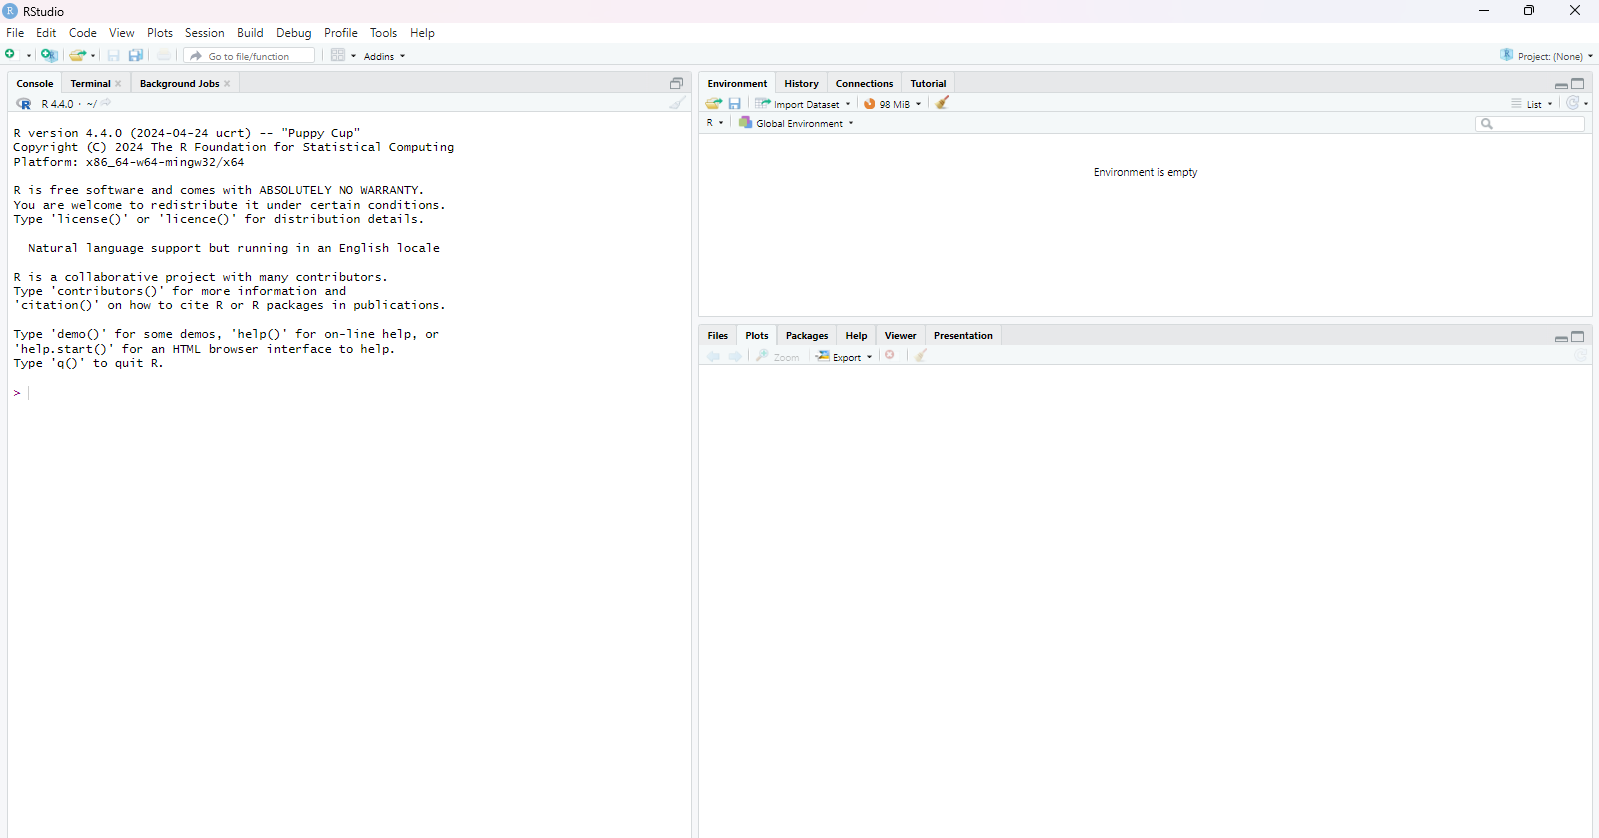
\includegraphics[width=5.33in,height=\textheight,keepaspectratio]{img/chap1/rw1.png}

Step 2: To obtain the source or script editor use the following steps:

File \textgreater{} New File \textgreater{} R Script

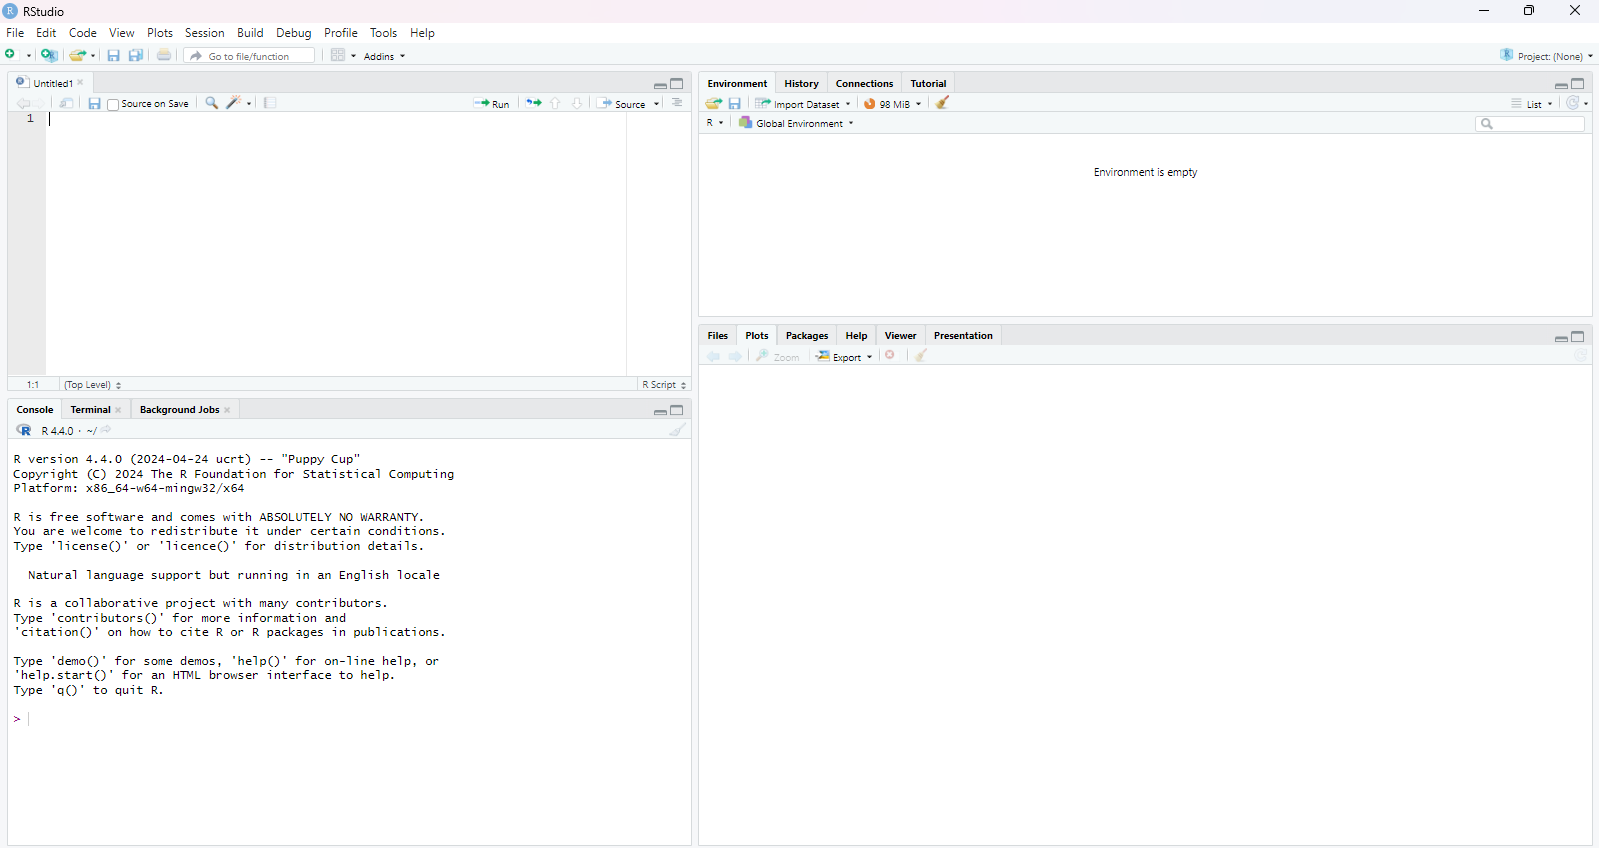
\includegraphics[width=5.33in,height=\textheight,keepaspectratio]{img/chap1/rw2.png}

Now we have four window. They are as follows:

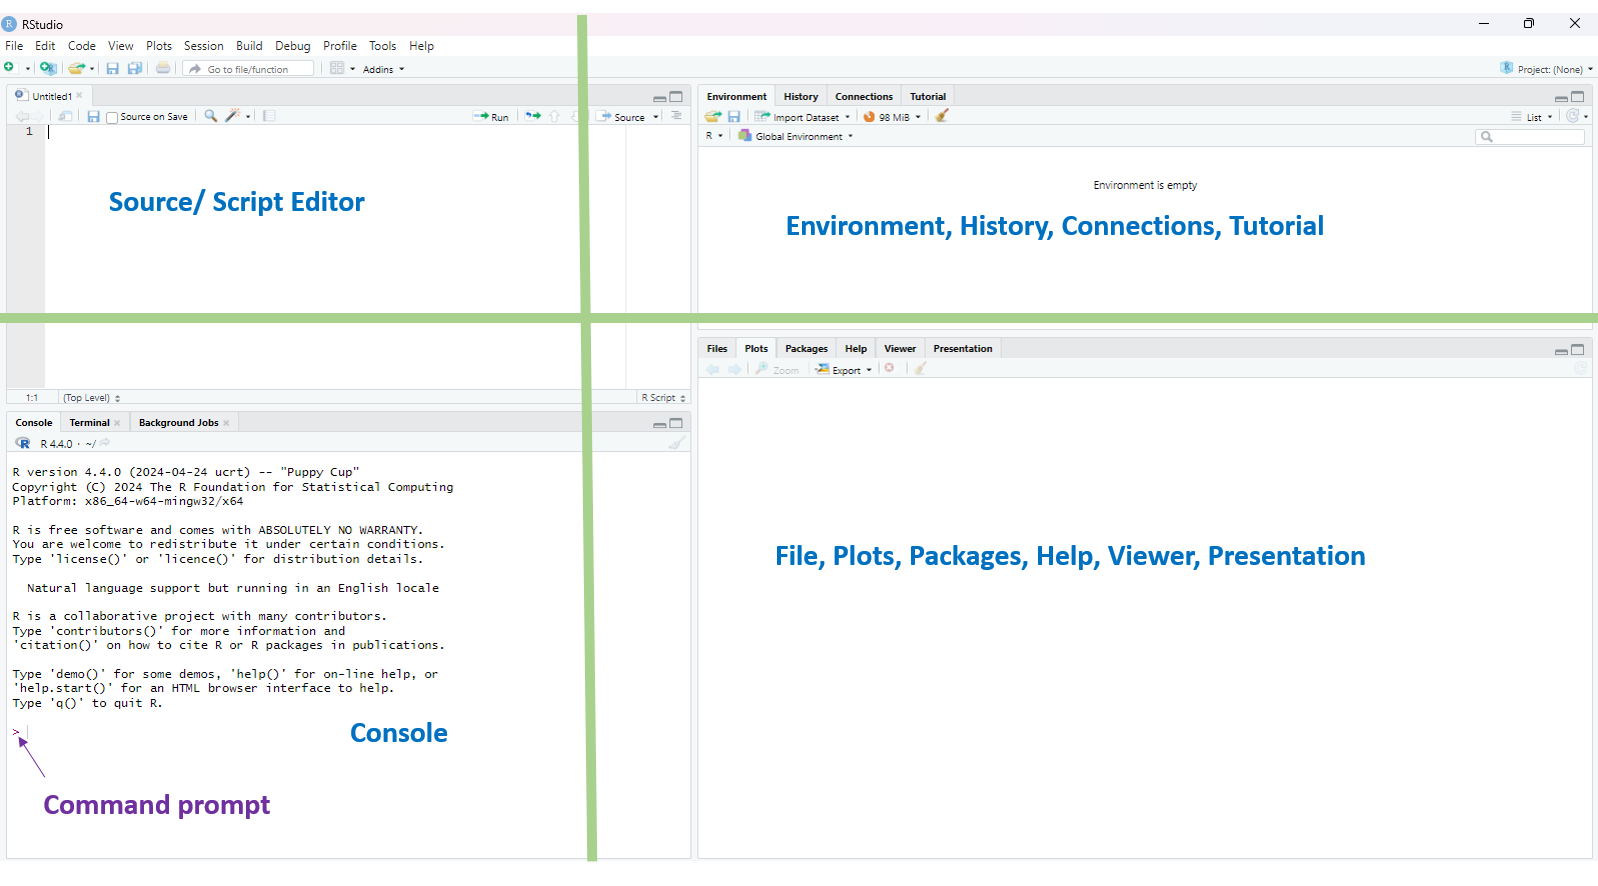
\includegraphics[width=5.33in,height=\textheight,keepaspectratio]{img/chap1/rw5.png}

\begin{enumerate}
\def\labelenumi{\arabic{enumi}.}
\tightlist
\item
  Source window: Here you can write your R codes.
\item
  Console: This is where you execute your commands to obtain the
  outputs.
\item
  Environment, History, Connections, Tutorial: Out of the different tabs
  you see here, the most important ones are the environment and the
  history tab.

  \begin{itemize}
  \item
    The Environment pane shows all the objects (like data frames,
    variables, functions, etc.) that are currently in your R session.
  \item
    The History tab keeps a record of all the commands you have run in
    the Console.
  \end{itemize}
\item
  File, Plots, Packages, Help, Viewer, Presentations:

  \begin{itemize}
  \item
    Files allows you to navigate your files.
  \item
    The graphical outputs are displayed here.
  \item
    Allows users to install, update, load, unload packages
  \item
    Help files corresponds to the functions are shown here. Help files
    provides function descriptions, examples and references for you to
    learn on your own. To access the help file of a function type ``?''
    followed by the function name . For example, `?ls`.
  \item
    Viewer/ Presentations: Useful when working with RMarkdown or Quarto
    documentations. We will look at this in Chapter 8.
  \end{itemize}
\end{enumerate}

\section{Change the appearance of RStudio
pane}\label{change-the-appearance-of-rstudio-pane}

This is an optional step. To change the appearance, font size, RStudio
theme colour follow the steps below:

Step 1: Go to Tools \textgreater{} Global Options. You will get the
window below

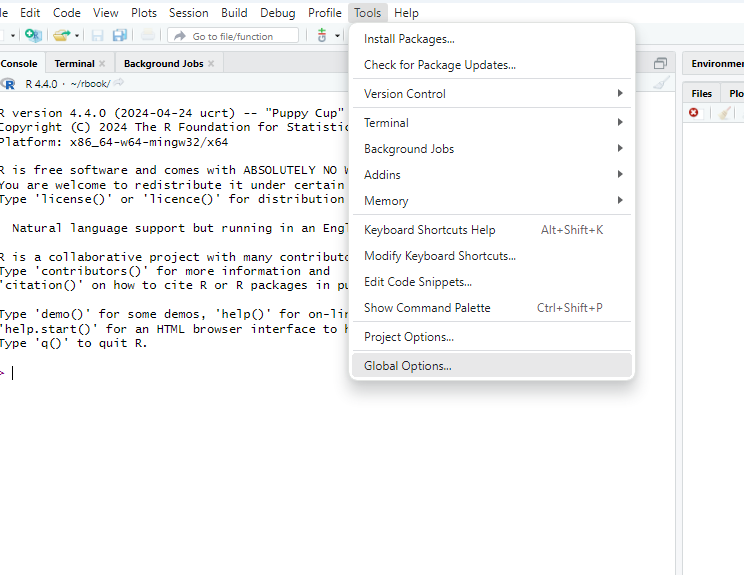
\includegraphics[width=2.48in,height=\textheight,keepaspectratio]{img/chap1/rw6.png}

Step 2: Select Appearance tab

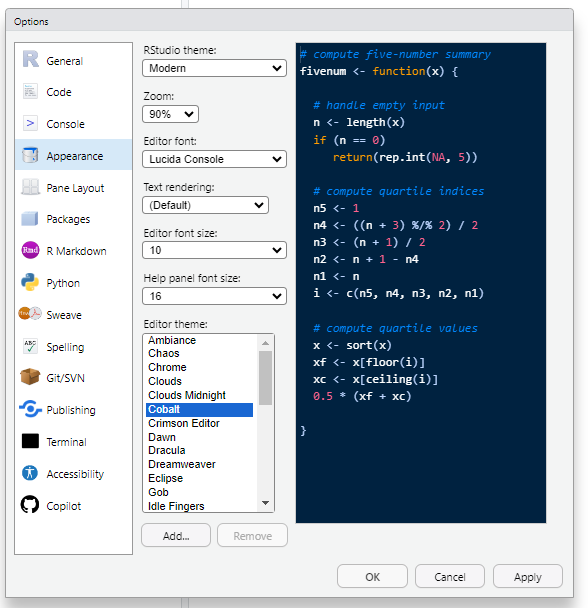
\includegraphics[width=1.96in,height=\textheight,keepaspectratio]{img/chap1/rw7.png}

Here, I select the theme to ``Cobalt''. Then the appearance of the
window will change as below:

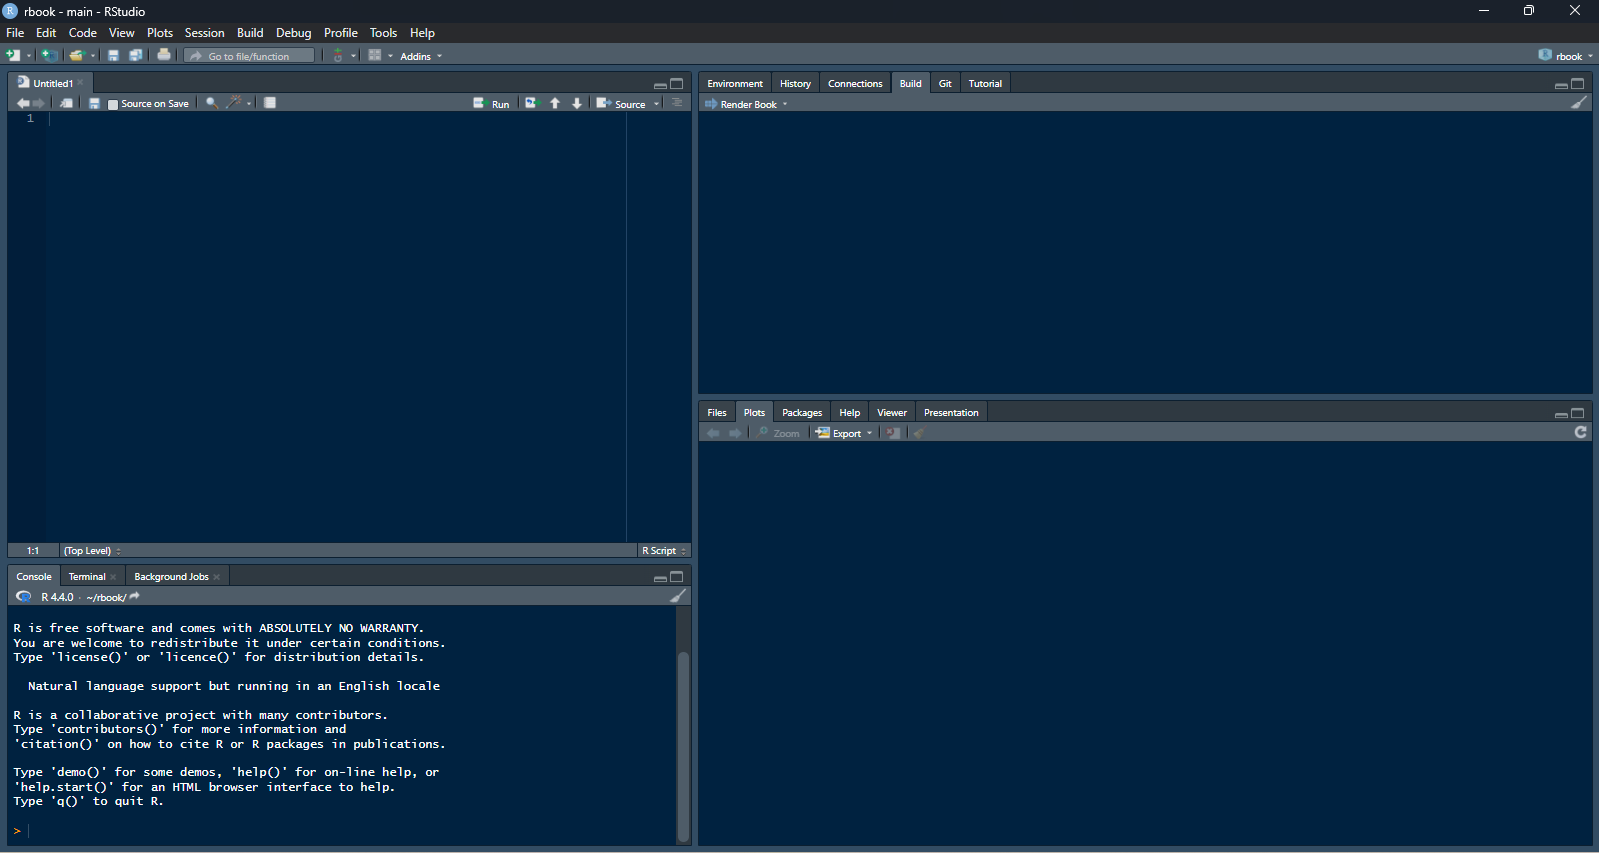
\includegraphics[width=5.33in,height=\textheight,keepaspectratio]{img/chap1/rw12.png}

\section{Creating an RStudio project}\label{creating-an-rstudio-project}

To create an RStudio project, please follow the following steps

Step 1: File \textgreater{} New Projects

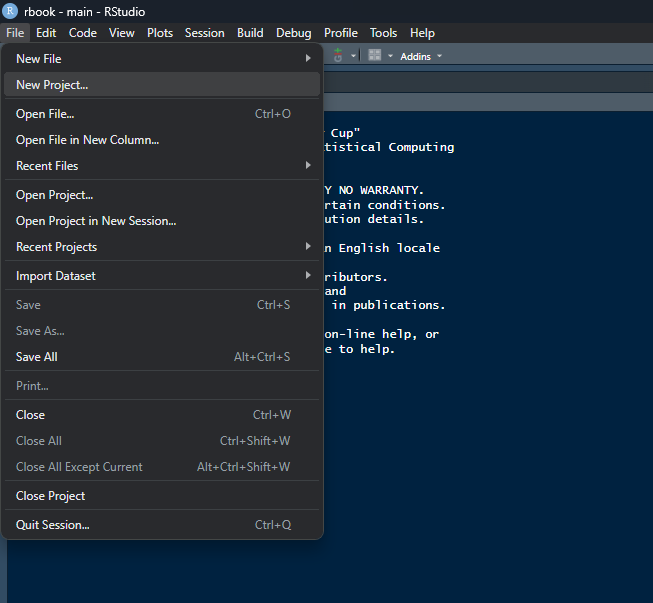
\includegraphics[width=2.18in,height=\textheight,keepaspectratio]{img/chap1/rw8.png}

Step 2: Click on the ``New Directory'' on the following window.

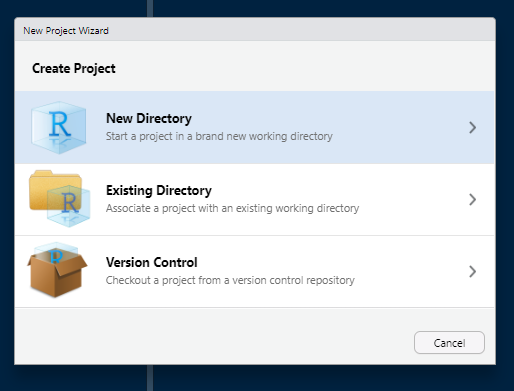
\includegraphics[width=1.71in,height=\textheight,keepaspectratio]{img/chap1/rw9.png}

Step 3: Click on ``New Project''

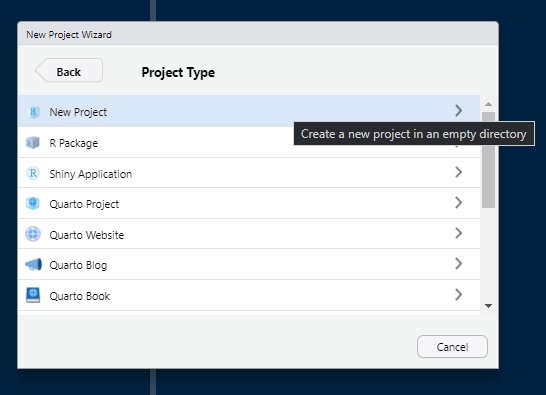
\includegraphics[width=1.82in,height=\textheight,keepaspectratio]{img/chap1/rw10.png}

Step 4: Give a directory name and a path to save

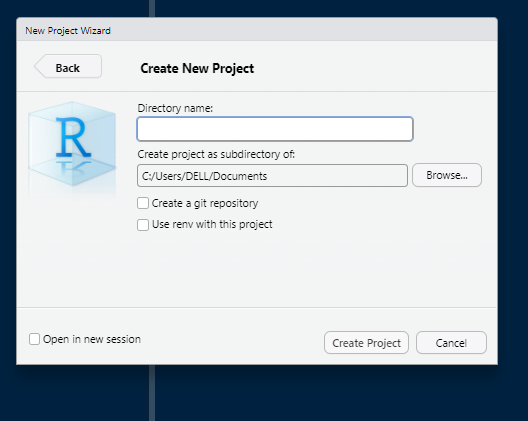
\includegraphics[width=1.76in,height=\textheight,keepaspectratio]{img/chap1/rw11.png}

\section{To save an R Studio
projects}\label{to-save-an-r-studio-projects}

\textbf{Category 1:} If you have created a project using the steps shown
in Section 1.10, you can save your R Script files by clicking on the
floppy disk icon, as illustrated in the figure below:

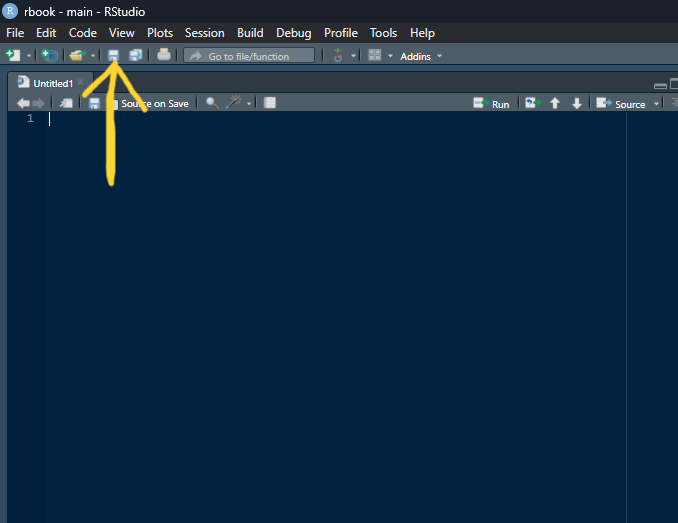
\includegraphics[width=2.26in,height=\textheight,keepaspectratio]{img/chap1/rw13.png}

\textbf{Category 2:} If you started coding without creating a project
and want to save your work, go to File \textgreater{} Save As and follow
the steps.

\section{Exercise}\label{exercise}

The goal of this exercise is to help you become familiar with the R
Studio environment and create and save projects.

\begin{enumerate}
\def\labelenumi{\arabic{enumi}.}
\item
  Create a new project in the RStudio IDE. Name your project as lesson1.
\item
  Select a suitable theme for your RStudio IDE's user interface.
\end{enumerate}

\begin{quote}
Help: Navigate to Tools \textgreater{} Global Options \textgreater{}
Appearance .
\end{quote}

\begin{enumerate}
\def\labelenumi{\arabic{enumi}.}
\setcounter{enumi}{2}
\tightlist
\item
  Change the RStudio pane layout as follows:
\end{enumerate}

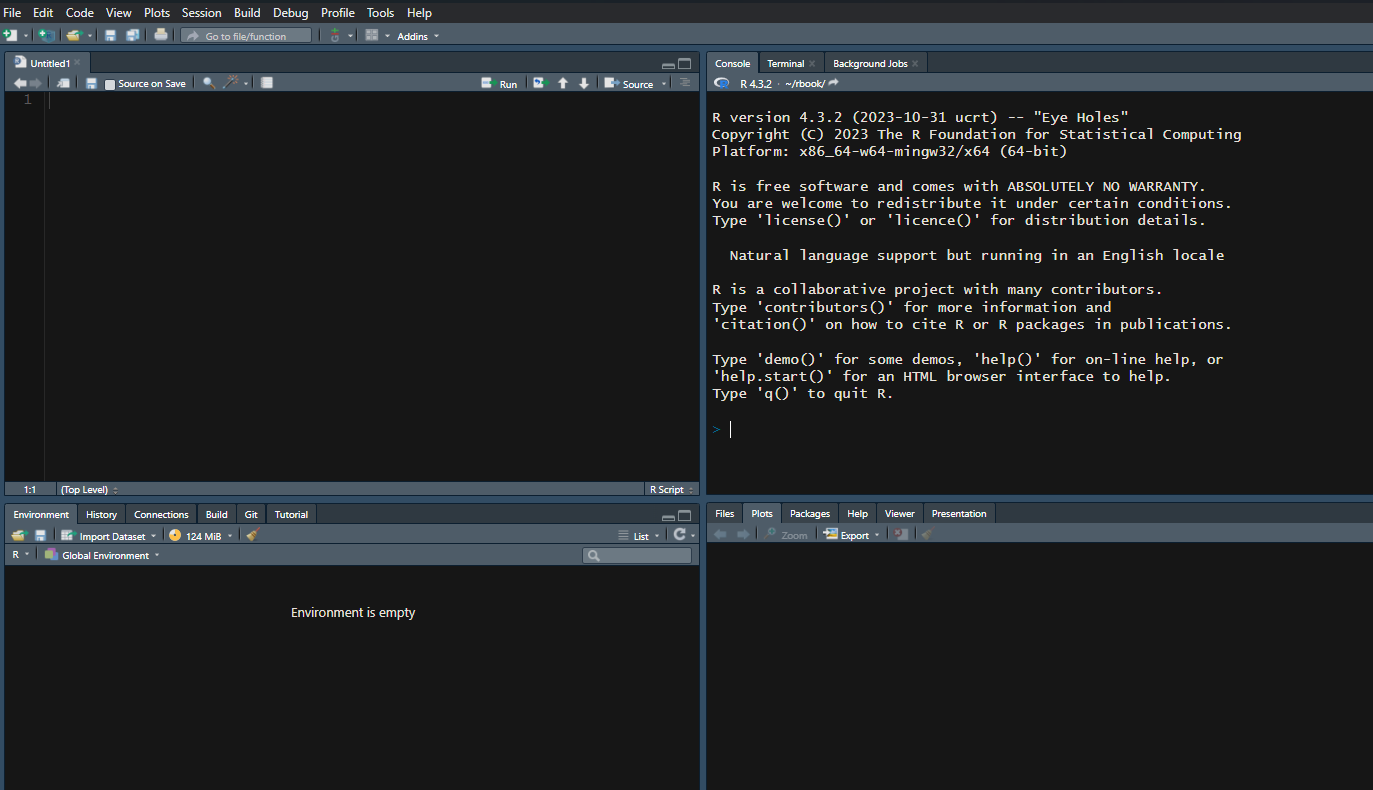
\includegraphics[width=4.58in,height=\textheight,keepaspectratio]{ch1.png}

\begin{enumerate}
\def\labelenumi{\arabic{enumi}.}
\setcounter{enumi}{3}
\item
  Create a folder called \texttt{data} inside your lesson1 project
  folder.
\item
  Create another folder called \texttt{src} inside your lesson1 project
  folder.
\item
  Open a script file and save it as \texttt{exercise1.R} inside the src
  folder.
\item
  Type the following commands on \texttt{exercise1.R} and run it on the
  console. See the changes happening under the ``Environment'' tab and
  the ``History'' tab.
\end{enumerate}

\begin{Shaded}
\begin{Highlighting}[]
\DecValTok{100} \SpecialCharTok{+} \DecValTok{200}
\FunctionTok{rnorm}\NormalTok{(}\DecValTok{100}\NormalTok{)}
\NormalTok{grades }\OtherTok{\textless{}{-}} \FunctionTok{c}\NormalTok{(}\StringTok{"A+"}\NormalTok{, }\StringTok{"A{-}"}\NormalTok{, }\StringTok{"A"}\NormalTok{, }\StringTok{"B"}\NormalTok{, }\StringTok{"F"}\NormalTok{)}
\NormalTok{random.numbers }\OtherTok{\textless{}{-}} \FunctionTok{rnorm}\NormalTok{(}\DecValTok{100}\NormalTok{)}
\NormalTok{random.numbers}\SpecialCharTok{*}\DecValTok{100}
\FunctionTok{ls}\NormalTok{()}
\end{Highlighting}
\end{Shaded}

\begin{enumerate}
\def\labelenumi{\arabic{enumi}.}
\setcounter{enumi}{7}
\item
  Close the project by saving the workspace.
\item
  Reopen your project by clicking the leason1.Rproj inside your lesson1
  folder. Open the .RData file and the .Rhistory file and observe them.
\item
  Type the following commands on exercise1.R and run them on the
  console.
\end{enumerate}

\begin{Shaded}
\begin{Highlighting}[]
\NormalTok{marks }\OtherTok{\textless{}{-}} \FunctionTok{c}\NormalTok{(}\DecValTok{100}\NormalTok{, }\DecValTok{70}\NormalTok{, }\DecValTok{80}\NormalTok{, }\DecValTok{60}\NormalTok{)}
\end{Highlighting}
\end{Shaded}

\begin{enumerate}
\def\labelenumi{\arabic{enumi}.}
\setcounter{enumi}{10}
\item
  Close the project without saving the workspace.
\item
  Reopen the lesson1.Rproj and type \texttt{ls()} on the console, and
  observe the output. (\texttt{marks} is not listed, but the other
  objects are available. Why?)
\item
  Type the following command in the console to observe changes in the
  console, environment, history, and Viewer windows. Observe the outputs
  of the code and gain an understanding of the purpose of each line.
\end{enumerate}

\begin{Shaded}
\begin{Highlighting}[]
\FunctionTok{data}\NormalTok{(}\StringTok{"iris"}\NormalTok{)}
\FunctionTok{View}\NormalTok{(iris)}
\FunctionTok{summary}\NormalTok{(iris)}
\FunctionTok{hist}\NormalTok{(iris}\SpecialCharTok{$}\NormalTok{Sepal.Length)}
\FunctionTok{plot}\NormalTok{(}\AttributeTok{x=}\NormalTok{iris}\SpecialCharTok{$}\NormalTok{Sepal.Length, }\AttributeTok{y=}\NormalTok{iris}\SpecialCharTok{$}\NormalTok{Sepal.Width) }\CommentTok{\# Method 1}
\FunctionTok{plot}\NormalTok{(Sepal.Length }\SpecialCharTok{\textasciitilde{}}\NormalTok{ Sepal.Width, }\AttributeTok{data=}\NormalTok{iris) }\CommentTok{\# Method 2}
\FunctionTok{plot}\NormalTok{(}\AttributeTok{x=}\NormalTok{iris}\SpecialCharTok{$}\NormalTok{Sepal.Length, }\AttributeTok{y=}\NormalTok{iris}\SpecialCharTok{$}\NormalTok{Sepal.Width, }\AttributeTok{col=}\NormalTok{iris}\SpecialCharTok{$}\NormalTok{Species) }
\FunctionTok{plot}\NormalTok{(Sepal.Length }\SpecialCharTok{\textasciitilde{}}\NormalTok{ Sepal.Width, }\AttributeTok{data=}\NormalTok{iris)}
\FunctionTok{plot}\NormalTok{(Sepal.Length }\SpecialCharTok{\textasciitilde{}}\NormalTok{ Sepal.Width, }\AttributeTok{pch=}\DecValTok{16}\NormalTok{, }\AttributeTok{cex=}\FloatTok{0.6}\NormalTok{, }\AttributeTok{data=}\NormalTok{iris)}
\FunctionTok{plot}\NormalTok{(Sepal.Length }\SpecialCharTok{\textasciitilde{}}\NormalTok{ Sepal.Width, }\AttributeTok{pch=}\DecValTok{16}\NormalTok{, }\AttributeTok{cex=}\FloatTok{0.6}\NormalTok{, }\AttributeTok{data=}\NormalTok{iris)}
\FunctionTok{plot}\NormalTok{(Sepal.Length }\SpecialCharTok{\textasciitilde{}}\NormalTok{ Sepal.Width, }\AttributeTok{col=}\StringTok{"forestgreen"}\NormalTok{, }\AttributeTok{pch=}\DecValTok{16}\NormalTok{, }\AttributeTok{cex=}\FloatTok{0.6}\NormalTok{, }\AttributeTok{data=}\NormalTok{iris)}
\end{Highlighting}
\end{Shaded}

\begin{enumerate}
\def\labelenumi{\arabic{enumi}.}
\setcounter{enumi}{13}
\tightlist
\item
  Type the following code to obtain list of predefined colours.
\end{enumerate}

\begin{Shaded}
\begin{Highlighting}[]
\FunctionTok{colours}\NormalTok{()}
\end{Highlighting}
\end{Shaded}

\begin{enumerate}
\def\labelenumi{\arabic{enumi}.}
\setcounter{enumi}{14}
\tightlist
\item
  Explore what changes the following code do on the last plot that you
  took.
\end{enumerate}

code chunk 15.1

\begin{Shaded}
\begin{Highlighting}[]
\FunctionTok{plot}\NormalTok{(Sepal.Length }\SpecialCharTok{\textasciitilde{}}\NormalTok{ Sepal.Width, }\AttributeTok{col=}\StringTok{"forestgreen"}\NormalTok{, }\AttributeTok{pch=}\DecValTok{16}\NormalTok{, }\AttributeTok{cex=}\FloatTok{0.6}\NormalTok{, }\AttributeTok{data=}\NormalTok{iris, }\AttributeTok{main =} \StringTok{"Scatterplot Between Sepal Length and Petal Length"}\NormalTok{,}
     \AttributeTok{xlab =} \StringTok{"Sepal Length (cm)"}\NormalTok{,}
     \AttributeTok{ylab =} \StringTok{"Sepal Width (cm)"}\NormalTok{)}
\end{Highlighting}
\end{Shaded}

code chunk 15.2

\begin{Shaded}
\begin{Highlighting}[]
\NormalTok{model }\OtherTok{\textless{}{-}} \FunctionTok{lm}\NormalTok{(Sepal.Length }\SpecialCharTok{\textasciitilde{}}\NormalTok{ Sepal.Width, }\AttributeTok{data=}\NormalTok{iris)}
\FunctionTok{plot}\NormalTok{(Sepal.Length }\SpecialCharTok{\textasciitilde{}}\NormalTok{ Sepal.Width, }\AttributeTok{col=}\StringTok{"forestgreen"}\NormalTok{, }\AttributeTok{pch=}\DecValTok{16}\NormalTok{, }\AttributeTok{cex=}\FloatTok{0.6}\NormalTok{, }\AttributeTok{data=}\NormalTok{iris, }\AttributeTok{main =} \StringTok{"Scatterplot Between Sepal Length and Petal Length"}\NormalTok{,}
     \AttributeTok{xlab =} \StringTok{"Sepal Length (cm)"}\NormalTok{,}
     \AttributeTok{ylab =} \StringTok{"Sepal Width (cm)"}\NormalTok{)}
\FunctionTok{abline}\NormalTok{(model, }\AttributeTok{col=}\StringTok{"tomato1"}\NormalTok{)}
\end{Highlighting}
\end{Shaded}

\begin{enumerate}
\def\labelenumi{\arabic{enumi}.}
\setcounter{enumi}{15}
\tightlist
\item
  Type the following commands and understand what each line of code is
  doing. Interpret the outputs.
\end{enumerate}

code chunk 16.1

\begin{Shaded}
\begin{Highlighting}[]
\FunctionTok{plot}\NormalTok{(iris)}
\end{Highlighting}
\end{Shaded}

code chunk 16.2

\begin{Shaded}
\begin{Highlighting}[]
\FunctionTok{plot}\NormalTok{(}\SpecialCharTok{\textasciitilde{}}\NormalTok{ Petal.Length }\SpecialCharTok{+}\NormalTok{ Petal.Width }\SpecialCharTok{+}\NormalTok{ Sepal.Width, }\AttributeTok{data=}\NormalTok{iris)}
\end{Highlighting}
\end{Shaded}

\begin{enumerate}
\def\labelenumi{\arabic{enumi}.}
\setcounter{enumi}{16}
\tightlist
\item
  Type the following command and open your data folder and see the
  changes that had occurred.
\end{enumerate}

\begin{Shaded}
\begin{Highlighting}[]
\FunctionTok{write.csv}\NormalTok{(iris, }\AttributeTok{file=}\StringTok{"data/iris.csv"}\NormalTok{)}
\end{Highlighting}
\end{Shaded}

\bookmarksetup{startatroot}

\chapter{Data Structures}\label{data-structures}

There are five main data structures in R. They are:

\begin{enumerate}
\def\labelenumi{\arabic{enumi}.}
\item
  vectors
\item
  matrix
\item
  array
\item
  data frame
\item
  list
\end{enumerate}

\section{Vectors}\label{vectors}

\begin{enumerate}
\def\labelenumi{\arabic{enumi}.}
\item
  One dimensional data object.
\item
  Homogeneous data structure. That means data in a vector must only be
  one type or mode (numeric, character, or logical). You cannot mix
  different types of data. If you try to mix different types of data, R
  will automatically convert them into one type.
\end{enumerate}

\subsection{Creating Vectors}\label{creating-vectors}

Vectors can be made in four primary ways. They are

\begin{enumerate}
\def\labelenumi{\roman{enumi}.}
\item
  using \texttt{c()} function
\item
  using \texttt{:} function
\item
  using \texttt{seq} function
\item
  using \texttt{rep} function
\end{enumerate}

Methods ii--iv simplify vector creation. They are useful when there is a
pattern in data.

\subsection{\texorpdfstring{Concatenate:
\texttt{c()}}{Concatenate: c()}}\label{concatenate-c}

syntax:

Example:

The following will create the vector but not assigned a name.

\begin{Shaded}
\begin{Highlighting}[]
\FunctionTok{c}\NormalTok{(}\DecValTok{1996}\NormalTok{, }\DecValTok{1998}\NormalTok{, }\DecValTok{2000}\NormalTok{, }\DecValTok{2005}\NormalTok{)}
\end{Highlighting}
\end{Shaded}

\begin{verbatim}
[1] 1996 1998 2000 2005
\end{verbatim}

Assigning a name to vector:

The advantage of assigning a name is that we can reuse the same set of
values by calling the vector name.

\begin{Shaded}
\begin{Highlighting}[]
\NormalTok{a }\OtherTok{\textless{}{-}} \FunctionTok{c}\NormalTok{(}\DecValTok{1996}\NormalTok{, }\DecValTok{1998}\NormalTok{, }\DecValTok{2000}\NormalTok{, }\DecValTok{2005}\NormalTok{)}
\NormalTok{a}
\end{Highlighting}
\end{Shaded}

\begin{verbatim}
[1] 1996 1998 2000 2005
\end{verbatim}

\subsection{\texorpdfstring{Colon: \texttt{:}}{Colon: :}}\label{colon}

The \texttt{:} function can be used to create a regular decreasing or
increasing sequence.

Examples:

\begin{Shaded}
\begin{Highlighting}[]
\DecValTok{1}\SpecialCharTok{:}\DecValTok{10}
\end{Highlighting}
\end{Shaded}

\begin{verbatim}
 [1]  1  2  3  4  5  6  7  8  9 10
\end{verbatim}

\begin{Shaded}
\begin{Highlighting}[]
\DecValTok{10}\SpecialCharTok{:}\DecValTok{1}
\end{Highlighting}
\end{Shaded}

\begin{verbatim}
 [1] 10  9  8  7  6  5  4  3  2  1
\end{verbatim}

\begin{Shaded}
\begin{Highlighting}[]
\SpecialCharTok{{-}}\FloatTok{0.5}\SpecialCharTok{:}\DecValTok{10}
\end{Highlighting}
\end{Shaded}

\begin{verbatim}
 [1] -0.5  0.5  1.5  2.5  3.5  4.5  5.5  6.5  7.5  8.5  9.5
\end{verbatim}

\begin{Shaded}
\begin{Highlighting}[]
\SpecialCharTok{{-}}\FloatTok{0.3}\SpecialCharTok{:}\DecValTok{10}
\end{Highlighting}
\end{Shaded}

\begin{verbatim}
 [1] -0.3  0.7  1.7  2.7  3.7  4.7  5.7  6.7  7.7  8.7  9.7
\end{verbatim}

In all of the above sequences the increment is one. The output will
display the numbers only within the range.

\subsection{\texorpdfstring{Sequence:
\texttt{seq}}{Sequence: seq}}\label{sequence-seq}

\texttt{seq} function cal also be used for creating regular sequence.
With \texttt{seq} you can control the increment and length of the
output.

\textbf{Example 1}

\begin{Shaded}
\begin{Highlighting}[]
\FunctionTok{seq}\NormalTok{(}\DecValTok{1}\NormalTok{, }\DecValTok{19}\NormalTok{)}
\end{Highlighting}
\end{Shaded}

\begin{verbatim}
 [1]  1  2  3  4  5  6  7  8  9 10 11 12 13 14 15 16 17 18 19
\end{verbatim}

\textbf{Example 2}

\begin{Shaded}
\begin{Highlighting}[]
\FunctionTok{seq}\NormalTok{(}\DecValTok{1}\NormalTok{, }\DecValTok{19}\NormalTok{, }\AttributeTok{length.out=}\DecValTok{8}\NormalTok{)}
\end{Highlighting}
\end{Shaded}

\begin{verbatim}
[1]  1.000000  3.571429  6.142857  8.714286 11.285714 13.857143 16.428571
[8] 19.000000
\end{verbatim}

\textbf{Example 3}

\begin{Shaded}
\begin{Highlighting}[]
\FunctionTok{seq}\NormalTok{(}\DecValTok{1}\NormalTok{, }\DecValTok{19}\NormalTok{, }\AttributeTok{by =} \DecValTok{3}\NormalTok{)}
\end{Highlighting}
\end{Shaded}

\begin{verbatim}
[1]  1  4  7 10 13 16 19
\end{verbatim}

\subsection{\texorpdfstring{Repeat:
\texttt{rep}}{Repeat: rep}}\label{repeat-rep}

The \texttt{rep} function can be used if there is a pattern of
repetition in the data.

\textbf{Example 1}

The number 8 is repeated three times.

\begin{Shaded}
\begin{Highlighting}[]
\FunctionTok{rep}\NormalTok{(}\DecValTok{8}\NormalTok{, }\DecValTok{5}\NormalTok{)}
\end{Highlighting}
\end{Shaded}

\begin{verbatim}
[1] 8 8 8 8 8
\end{verbatim}

\textbf{Example 2}

The sequence \texttt{1,\ 2,\ 3} is repeated five times.

\begin{Shaded}
\begin{Highlighting}[]
\FunctionTok{rep}\NormalTok{(}\DecValTok{1}\SpecialCharTok{:}\DecValTok{3}\NormalTok{, }\AttributeTok{times=}\DecValTok{5}\NormalTok{)}
\end{Highlighting}
\end{Shaded}

\begin{verbatim}
 [1] 1 2 3 1 2 3 1 2 3 1 2 3 1 2 3
\end{verbatim}

\textbf{Example 3}

Same as in Example 2 above.

\begin{Shaded}
\begin{Highlighting}[]
\FunctionTok{rep}\NormalTok{(}\DecValTok{1}\SpecialCharTok{:}\DecValTok{3}\NormalTok{, }\DecValTok{5}\NormalTok{)}
\end{Highlighting}
\end{Shaded}

\begin{verbatim}
 [1] 1 2 3 1 2 3 1 2 3 1 2 3 1 2 3
\end{verbatim}

\textbf{Example 4}

Each element in the sequence is repeated five times.

\begin{Shaded}
\begin{Highlighting}[]
\FunctionTok{rep}\NormalTok{(}\DecValTok{1}\SpecialCharTok{:}\DecValTok{3}\NormalTok{, }\AttributeTok{each=}\DecValTok{5}\NormalTok{)}
\end{Highlighting}
\end{Shaded}

\begin{verbatim}
 [1] 1 1 1 1 1 2 2 2 2 2 3 3 3 3 3
\end{verbatim}

\textbf{Example 5}

First, each element is repeated five times. After that, the whole
sequence is repeated three times.

\begin{Shaded}
\begin{Highlighting}[]
\FunctionTok{rep}\NormalTok{(}\DecValTok{1}\SpecialCharTok{:}\DecValTok{3}\NormalTok{, }\AttributeTok{each=}\DecValTok{5}\NormalTok{, }\AttributeTok{times=}\DecValTok{3}\NormalTok{)}
\end{Highlighting}
\end{Shaded}

\begin{verbatim}
 [1] 1 1 1 1 1 2 2 2 2 2 3 3 3 3 3 1 1 1 1 1 2 2 2 2 2 3 3 3 3 3 1 1 1 1 1 2 2 2
[39] 2 2 3 3 3 3 3
\end{verbatim}

\textbf{Example 6}

Same as before. Changing the ordering of \texttt{each} and \texttt{time}
does not change the output.

\begin{Shaded}
\begin{Highlighting}[]
\FunctionTok{rep}\NormalTok{(}\DecValTok{1}\SpecialCharTok{:}\DecValTok{3}\NormalTok{, }\AttributeTok{times=}\DecValTok{3}\NormalTok{, }\AttributeTok{each=}\DecValTok{5}\NormalTok{)}
\end{Highlighting}
\end{Shaded}

\begin{verbatim}
 [1] 1 1 1 1 1 2 2 2 2 2 3 3 3 3 3 1 1 1 1 1 2 2 2 2 2 3 3 3 3 3 1 1 1 1 1 2 2 2
[39] 2 2 3 3 3 3 3
\end{verbatim}

\subsection{Coercion}\label{coercion}

When you try to include different types they will be coerced to the most
flexible type.

\begin{Shaded}
\begin{Highlighting}[]
\NormalTok{a }\OtherTok{\textless{}{-}} \FunctionTok{c}\NormalTok{(}\DecValTok{1}\NormalTok{, }\DecValTok{3}\NormalTok{, }\StringTok{"GPA"}\NormalTok{, }\ConstantTok{TRUE}\NormalTok{, }\DecValTok{1}\NormalTok{L)}
\FunctionTok{typeof}\NormalTok{(a)}
\end{Highlighting}
\end{Shaded}

\begin{verbatim}
[1] "character"
\end{verbatim}

Explicit coercion means that if we try to convert a data type to another
data type intentionally using a specific function. For example,

\begin{Shaded}
\begin{Highlighting}[]
\NormalTok{b }\OtherTok{\textless{}{-}} \FunctionTok{c}\NormalTok{(}\FloatTok{3.1}\NormalTok{, }\FloatTok{3.2}\NormalTok{, }\FloatTok{3.7}\NormalTok{, }\FloatTok{5.9}\NormalTok{)}
\NormalTok{b}
\end{Highlighting}
\end{Shaded}

\begin{verbatim}
[1] 3.1 3.2 3.7 5.9
\end{verbatim}

\begin{Shaded}
\begin{Highlighting}[]
\FunctionTok{as.integer}\NormalTok{(b)}
\end{Highlighting}
\end{Shaded}

\begin{verbatim}
[1] 3 3 3 5
\end{verbatim}

\subsection{Functions that can be used to inspect
vectors}\label{functions-that-can-be-used-to-inspect-vectors}

Consider the vector below

\begin{Shaded}
\begin{Highlighting}[]
\NormalTok{example.vec }\OtherTok{\textless{}{-}} \FunctionTok{c}\NormalTok{(}\DecValTok{1}\NormalTok{,  }\DecValTok{2}\NormalTok{,  }\DecValTok{3}\NormalTok{, }\DecValTok{4}\NormalTok{, }\DecValTok{5}\NormalTok{, }\DecValTok{6}\NormalTok{, }\DecValTok{7}\NormalTok{, }\DecValTok{8}\NormalTok{)}
\end{Highlighting}
\end{Shaded}

\begin{enumerate}
\def\labelenumi{\arabic{enumi}.}
\tightlist
\item
  To check the storage mode
\end{enumerate}

\begin{Shaded}
\begin{Highlighting}[]
\FunctionTok{typeof}\NormalTok{(example.vec)}
\end{Highlighting}
\end{Shaded}

\begin{verbatim}
[1] "double"
\end{verbatim}

\begin{enumerate}
\def\labelenumi{\arabic{enumi}.}
\setcounter{enumi}{1}
\tightlist
\item
  To check the class type
\end{enumerate}

\begin{Shaded}
\begin{Highlighting}[]
\FunctionTok{class}\NormalTok{(example.vec)}
\end{Highlighting}
\end{Shaded}

\begin{verbatim}
[1] "numeric"
\end{verbatim}

\begin{enumerate}
\def\labelenumi{\arabic{enumi}.}
\setcounter{enumi}{2}
\tightlist
\item
  Testing functions
\end{enumerate}

\begin{Shaded}
\begin{Highlighting}[]
\FunctionTok{is.character}\NormalTok{(example.vec)}
\end{Highlighting}
\end{Shaded}

\begin{verbatim}
[1] FALSE
\end{verbatim}

\begin{Shaded}
\begin{Highlighting}[]
\FunctionTok{is.integer}\NormalTok{(example.vec)}
\end{Highlighting}
\end{Shaded}

\begin{verbatim}
[1] FALSE
\end{verbatim}

\begin{Shaded}
\begin{Highlighting}[]
\FunctionTok{is.logical}\NormalTok{(example.vec)}
\end{Highlighting}
\end{Shaded}

\begin{verbatim}
[1] FALSE
\end{verbatim}

\begin{Shaded}
\begin{Highlighting}[]
\FunctionTok{is.double}\NormalTok{(example.vec)}
\end{Highlighting}
\end{Shaded}

\begin{verbatim}
[1] TRUE
\end{verbatim}

\begin{enumerate}
\def\labelenumi{\arabic{enumi}.}
\setcounter{enumi}{3}
\tightlist
\item
  Mathematical and statistical functions
\end{enumerate}

\begin{Shaded}
\begin{Highlighting}[]
\FunctionTok{sum}\NormalTok{(example.vec)}
\end{Highlighting}
\end{Shaded}

\begin{verbatim}
[1] 36
\end{verbatim}

\begin{Shaded}
\begin{Highlighting}[]
\FunctionTok{mean}\NormalTok{(example.vec)}
\end{Highlighting}
\end{Shaded}

\begin{verbatim}
[1] 4.5
\end{verbatim}

\begin{Shaded}
\begin{Highlighting}[]
\FunctionTok{summary}\NormalTok{(example.vec)}
\end{Highlighting}
\end{Shaded}

\begin{verbatim}
   Min. 1st Qu.  Median    Mean 3rd Qu.    Max. 
   1.00    2.75    4.50    4.50    6.25    8.00 
\end{verbatim}

\begin{enumerate}
\def\labelenumi{\arabic{enumi}.}
\setcounter{enumi}{4}
\tightlist
\item
  To check if there are any missing values
\end{enumerate}

\begin{Shaded}
\begin{Highlighting}[]
\FunctionTok{is.na}\NormalTok{(example.vec)}
\end{Highlighting}
\end{Shaded}

\begin{verbatim}
[1] FALSE FALSE FALSE FALSE FALSE FALSE FALSE FALSE
\end{verbatim}

There are many more functions that you can use with vectors. We will
learn about them in the upcoming chapters.

\subsection{Exercise}\label{exercise-1}

\begin{enumerate}
\def\labelenumi{\arabic{enumi}.}
\tightlist
\item
  Write R codes to create the following vectors: If you see patterns in
  the data, use vector simplification methods.
\end{enumerate}

\begin{enumerate}
\def\labelenumi{\roman{enumi}.}
\tightlist
\item
\end{enumerate}

\begin{verbatim}
[1] 1990 1992 1934 1957 1970 2000 2005
\end{verbatim}

\begin{enumerate}
\def\labelenumi{\roman{enumi}.}
\setcounter{enumi}{1}
\tightlist
\item
\end{enumerate}

\begin{verbatim}
 [1] 3 6 9 3 6 9 3 6 9 3 6 9 3 6 9
\end{verbatim}

\begin{enumerate}
\def\labelenumi{\roman{enumi}.}
\setcounter{enumi}{2}
\tightlist
\item
\end{enumerate}

\begin{verbatim}
 [1] 3 3 3 3 3 6 6 6 6 6 9 9 9 9 9
\end{verbatim}

\begin{enumerate}
\def\labelenumi{\roman{enumi}.}
\setcounter{enumi}{3}
\tightlist
\item
\end{enumerate}

\begin{verbatim}
 [1] 3 3 3 3 3 6 6 6 6 6 9 9 9 9 9 3 3 3 3 3 6 6 6 6 6 9 9 9 9 9
\end{verbatim}

\begin{enumerate}
\def\labelenumi{\alph{enumi}.}
\setcounter{enumi}{21}
\tightlist
\item
\end{enumerate}

\begin{verbatim}
 [1]  1  4  7 10 13 16 19 22 25 28 31 34
\end{verbatim}

\begin{enumerate}
\def\labelenumi{\roman{enumi}.}
\setcounter{enumi}{5}
\tightlist
\item
\end{enumerate}

\begin{verbatim}
  [1] 0.1000000 0.1020202 0.1040404 0.1060606 0.1080808 0.1101010 0.1121212
  [8] 0.1141414 0.1161616 0.1181818 0.1202020 0.1222222 0.1242424 0.1262626
 [15] 0.1282828 0.1303030 0.1323232 0.1343434 0.1363636 0.1383838 0.1404040
 [22] 0.1424242 0.1444444 0.1464646 0.1484848 0.1505051 0.1525253 0.1545455
 [29] 0.1565657 0.1585859 0.1606061 0.1626263 0.1646465 0.1666667 0.1686869
 [36] 0.1707071 0.1727273 0.1747475 0.1767677 0.1787879 0.1808081 0.1828283
 [43] 0.1848485 0.1868687 0.1888889 0.1909091 0.1929293 0.1949495 0.1969697
 [50] 0.1989899 0.2010101 0.2030303 0.2050505 0.2070707 0.2090909 0.2111111
 [57] 0.2131313 0.2151515 0.2171717 0.2191919 0.2212121 0.2232323 0.2252525
 [64] 0.2272727 0.2292929 0.2313131 0.2333333 0.2353535 0.2373737 0.2393939
 [71] 0.2414141 0.2434343 0.2454545 0.2474747 0.2494949 0.2515152 0.2535354
 [78] 0.2555556 0.2575758 0.2595960 0.2616162 0.2636364 0.2656566 0.2676768
 [85] 0.2696970 0.2717172 0.2737374 0.2757576 0.2777778 0.2797980 0.2818182
 [92] 0.2838384 0.2858586 0.2878788 0.2898990 0.2919192 0.2939394 0.2959596
 [99] 0.2979798 0.3000000
\end{verbatim}

\begin{enumerate}
\def\labelenumi{\roman{enumi}.}
\setcounter{enumi}{6}
\tightlist
\item
\end{enumerate}

\begin{verbatim}
 [1] -0.5  0.5  1.5  2.5  3.5  4.5  5.5  6.5  7.5  8.5  9.5 10.5
\end{verbatim}

\begin{enumerate}
\def\labelenumi{\roman{enumi}.}
\setcounter{enumi}{7}
\tightlist
\item
\end{enumerate}

\begin{verbatim}
 [1]  2  4  6  8 10 12 14 16 18 20 22 24 26 28 30 32 34 36 38 40 42 44 46 48 50
[26] 52 54 56 58 60 62 64 66 68 70 72
\end{verbatim}

\begin{enumerate}
\def\labelenumi{\arabic{enumi}.}
\setcounter{enumi}{1}
\tightlist
\item
  Use the \texttt{typeof()} function to check the R storage mode of the
  following vectors and \texttt{class()} to check the class type of the
  vector.
\end{enumerate}

\begin{Shaded}
\begin{Highlighting}[]
\NormalTok{logical\_vector }\OtherTok{\textless{}{-}} \FunctionTok{c}\NormalTok{(}\ConstantTok{TRUE}\NormalTok{, }\ConstantTok{FALSE}\NormalTok{, }\ConstantTok{TRUE}\NormalTok{, }\ConstantTok{FALSE}\NormalTok{)}
\NormalTok{integer\_vector }\OtherTok{\textless{}{-}} \FunctionTok{c}\NormalTok{(}\DecValTok{1}\NormalTok{L, }\DecValTok{2}\NormalTok{L, }\DecValTok{3}\NormalTok{L, }\DecValTok{4}\NormalTok{L)}
\NormalTok{double\_vector }\OtherTok{\textless{}{-}} \FunctionTok{c}\NormalTok{(}\FloatTok{1.1}\NormalTok{, }\FloatTok{2.2}\NormalTok{, }\FloatTok{3.3}\NormalTok{, }\FloatTok{4.4}\NormalTok{)}
\NormalTok{complex\_vector }\OtherTok{\textless{}{-}} \FunctionTok{c}\NormalTok{(}\DecValTok{1}\SpecialCharTok{+}\DecValTok{1}\NormalTok{i, }\DecValTok{2}\SpecialCharTok{+}\DecValTok{2}\NormalTok{i, }\DecValTok{3}\SpecialCharTok{+}\DecValTok{3}\NormalTok{i, }\DecValTok{4}\SpecialCharTok{+}\DecValTok{4}\NormalTok{i)}
\NormalTok{character\_vector }\OtherTok{\textless{}{-}} \FunctionTok{c}\NormalTok{(}\StringTok{"a"}\NormalTok{, }\StringTok{"b"}\NormalTok{, }\StringTok{"c"}\NormalTok{, }\StringTok{"d"}\NormalTok{)}
\NormalTok{null\_vector }\OtherTok{\textless{}{-}} \ConstantTok{NULL}
\NormalTok{time\_data }\OtherTok{\textless{}{-}} \DecValTok{1996}\SpecialCharTok{:}\DecValTok{2006}
\NormalTok{time\_series\_data }\OtherTok{\textless{}{-}} \FunctionTok{ts}\NormalTok{(}\DecValTok{1996}\SpecialCharTok{:}\DecValTok{2006}\NormalTok{)}
\end{Highlighting}
\end{Shaded}

\begin{enumerate}
\def\labelenumi{\arabic{enumi}.}
\setcounter{enumi}{2}
\item
  Create the vector (3, 3, 3, . . . 3, 6, 6, . . . 6, 9, 9, 9, . . . 9),
  where there are 10 occurrences of 3, 20 occurrences of 6 and 30
  occurrences of 9.
\item
  Find the value of the following expression.
\end{enumerate}

\begin{enumerate}
\def\labelenumi{\roman{enumi}.}
\item
  \(\sum_{i=1}^{100}i\)
\item
  \(\sum_{i=1}^{100}i^2\)
\end{enumerate}

\begin{enumerate}
\def\labelenumi{\arabic{enumi}.}
\setcounter{enumi}{4}
\item
  Generate a sequence using the code seq(from=1, to=10, by=1). What
  other ways can you generate the same sequence?
\item
  Create a vector to hold population values, and label each element with
  the corresponding province name. The plot will display population
  values when hovered over.
\end{enumerate}

\pandocbounded{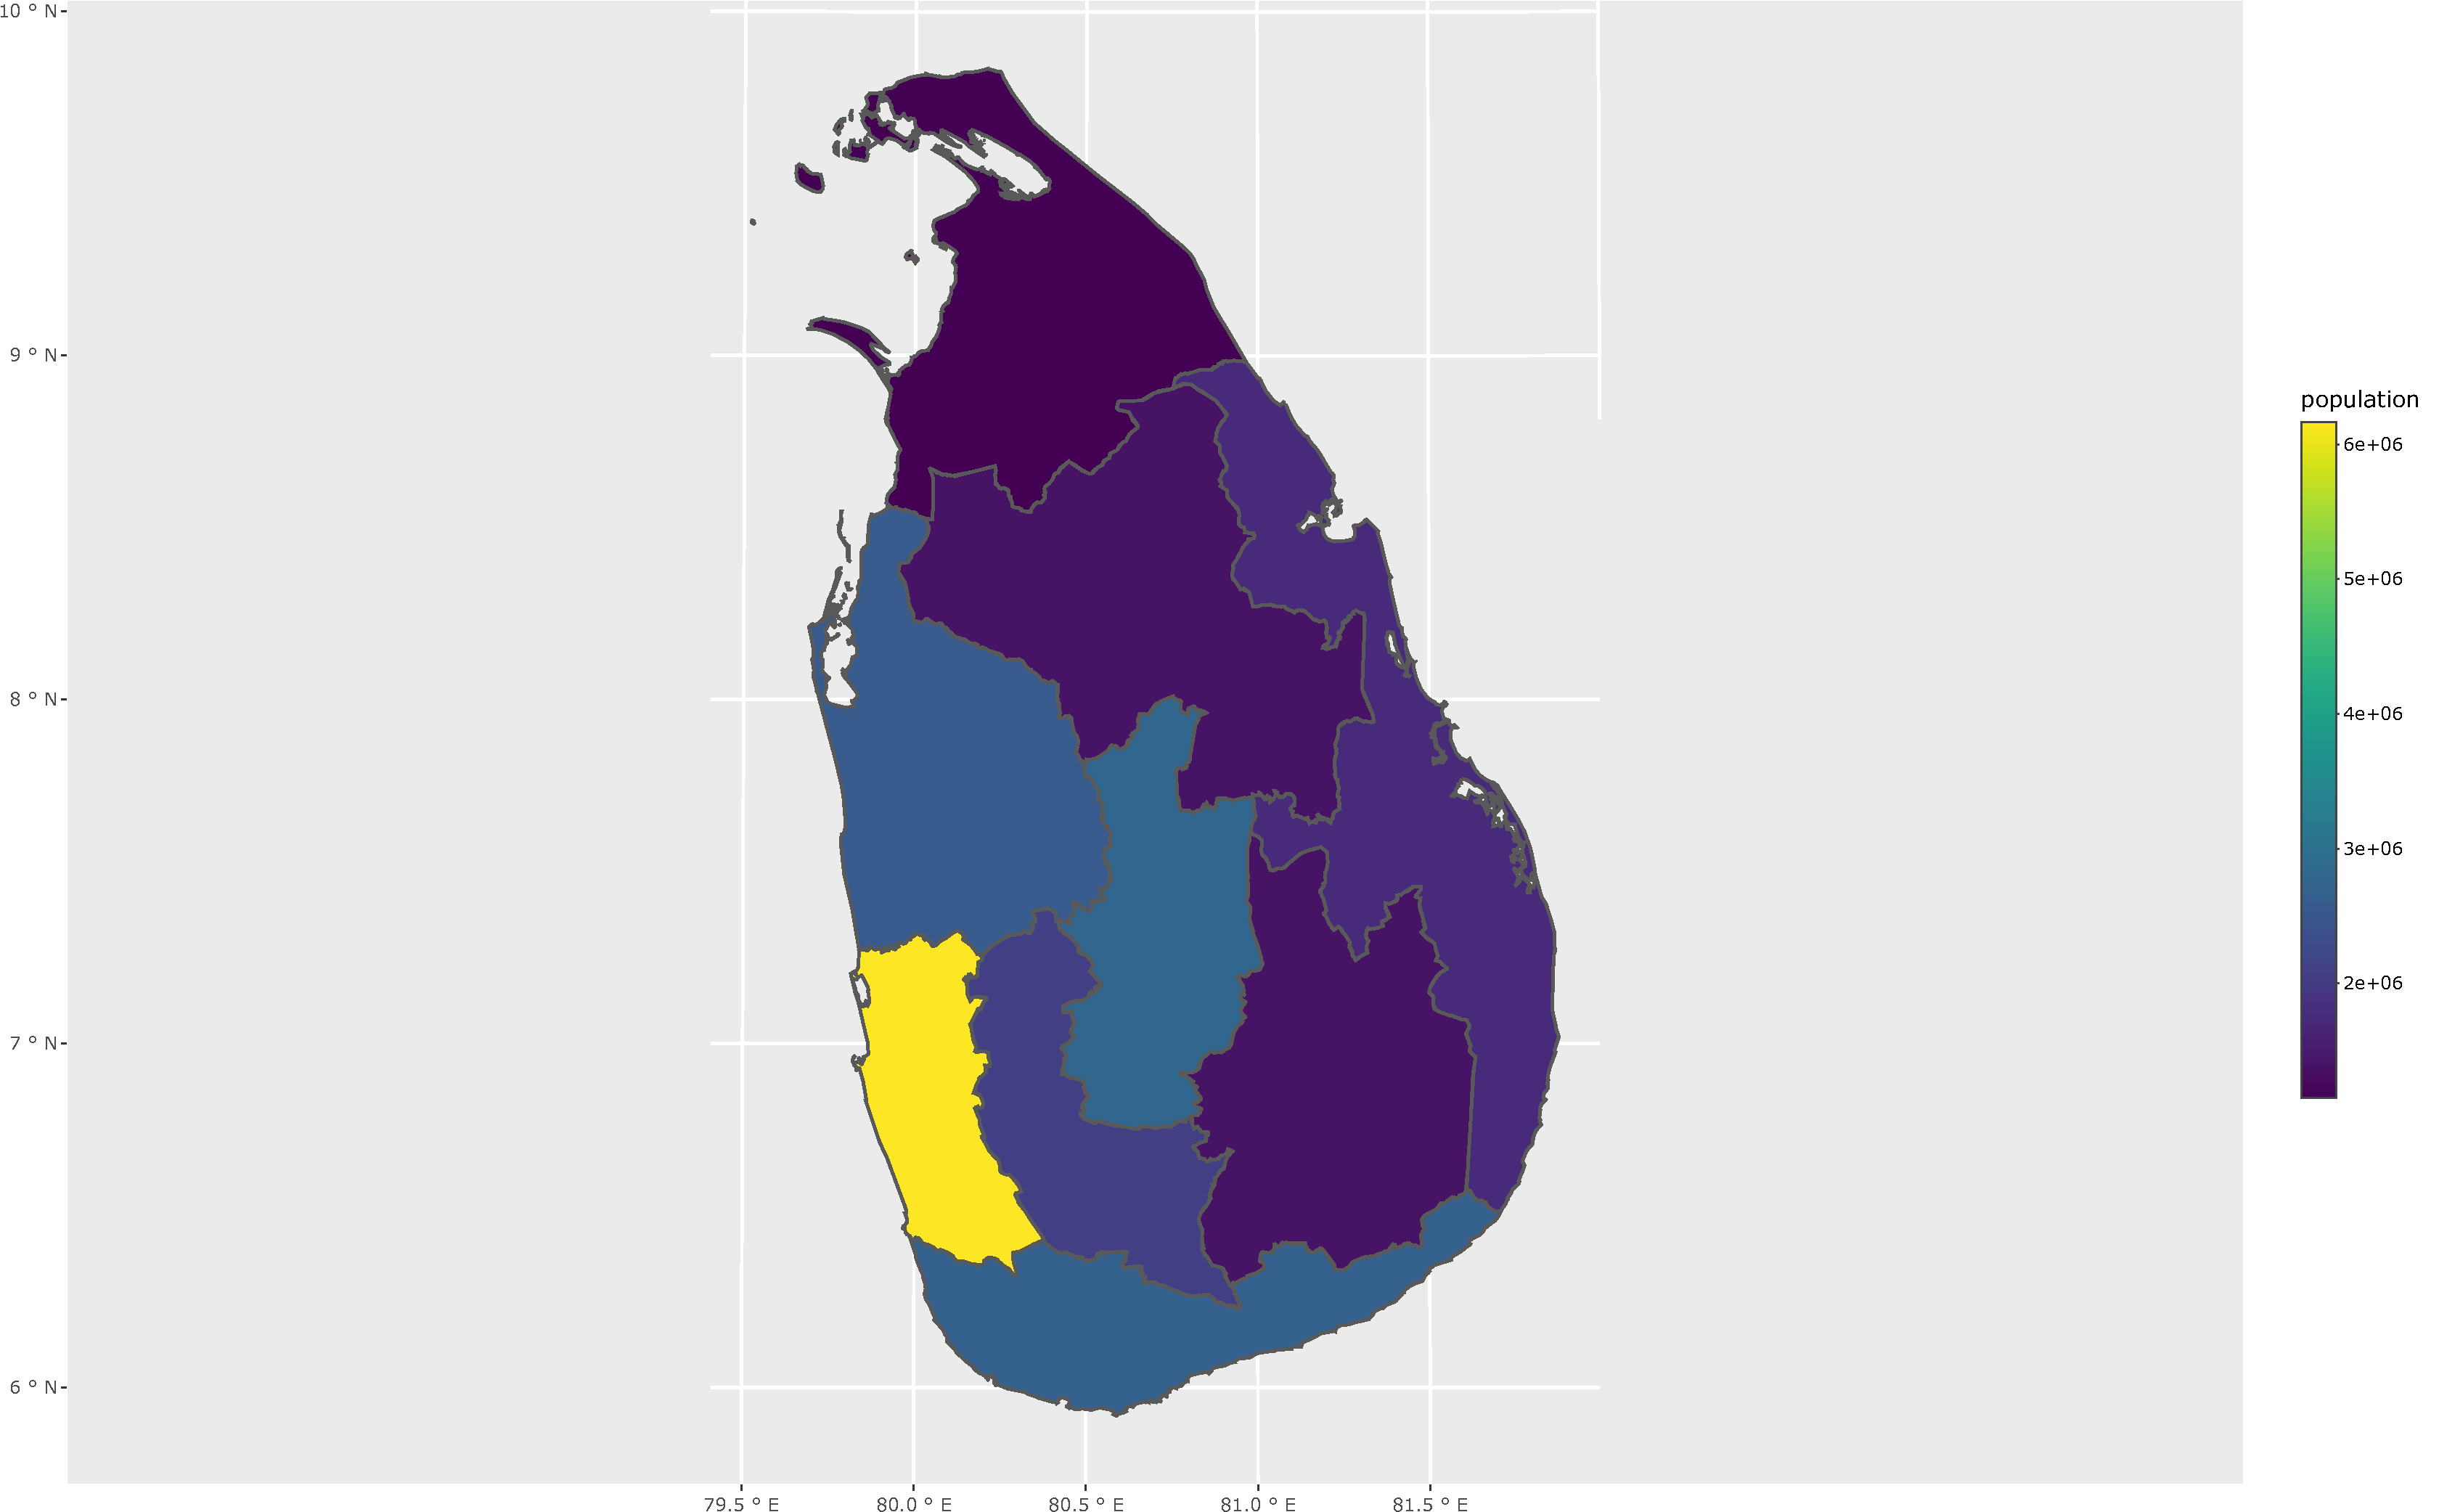
\includegraphics[keepaspectratio]{chap2_files/figure-pdf/unnamed-chunk-30-1.pdf}}

\subsection{Vector Operations}\label{vector-operations}

\begin{Shaded}
\begin{Highlighting}[]
\NormalTok{a }\OtherTok{\textless{}{-}} \DecValTok{1}\SpecialCharTok{:}\DecValTok{10}
\NormalTok{b }\OtherTok{\textless{}{-}} \FunctionTok{rep}\NormalTok{(}\DecValTok{10}\SpecialCharTok{:}\DecValTok{100}\NormalTok{, }\AttributeTok{by=}\DecValTok{10}\NormalTok{)}
\NormalTok{a }\SpecialCharTok{+}\NormalTok{ b}
\end{Highlighting}
\end{Shaded}

\begin{verbatim}
Warning in a + b: longer object length is not a multiple of shorter object
length
\end{verbatim}

\begin{verbatim}
 [1]  11  13  15  17  19  21  23  25  27  29  21  23  25  27  29  31  33  35  37
[20]  39  31  33  35  37  39  41  43  45  47  49  41  43  45  47  49  51  53  55
[39]  57  59  51  53  55  57  59  61  63  65  67  69  61  63  65  67  69  71  73
[58]  75  77  79  71  73  75  77  79  81  83  85  87  89  81  83  85  87  89  91
[77]  93  95  97  99  91  93  95  97  99 101 103 105 107 109 101
\end{verbatim}

\begin{Shaded}
\begin{Highlighting}[]
\NormalTok{a}\SpecialCharTok{/}\NormalTok{b}
\end{Highlighting}
\end{Shaded}

\begin{verbatim}
Warning in a/b: longer object length is not a multiple of shorter object length
\end{verbatim}

\begin{verbatim}
 [1] 0.10000000 0.18181818 0.25000000 0.30769231 0.35714286 0.40000000
 [7] 0.43750000 0.47058824 0.50000000 0.52631579 0.05000000 0.09523810
[13] 0.13636364 0.17391304 0.20833333 0.24000000 0.26923077 0.29629630
[19] 0.32142857 0.34482759 0.03333333 0.06451613 0.09375000 0.12121212
[25] 0.14705882 0.17142857 0.19444444 0.21621622 0.23684211 0.25641026
[31] 0.02500000 0.04878049 0.07142857 0.09302326 0.11363636 0.13333333
[37] 0.15217391 0.17021277 0.18750000 0.20408163 0.02000000 0.03921569
[43] 0.05769231 0.07547170 0.09259259 0.10909091 0.12500000 0.14035088
[49] 0.15517241 0.16949153 0.01666667 0.03278689 0.04838710 0.06349206
[55] 0.07812500 0.09230769 0.10606061 0.11940299 0.13235294 0.14492754
[61] 0.01428571 0.02816901 0.04166667 0.05479452 0.06756757 0.08000000
[67] 0.09210526 0.10389610 0.11538462 0.12658228 0.01250000 0.02469136
[73] 0.03658537 0.04819277 0.05952381 0.07058824 0.08139535 0.09195402
[79] 0.10227273 0.11235955 0.01111111 0.02197802 0.03260870 0.04301075
[85] 0.05319149 0.06315789 0.07291667 0.08247423 0.09183673 0.10101010
[91] 0.01000000
\end{verbatim}

\begin{Shaded}
\begin{Highlighting}[]
\NormalTok{a}\SpecialCharTok{*}\NormalTok{b}
\end{Highlighting}
\end{Shaded}

\begin{verbatim}
Warning in a * b: longer object length is not a multiple of shorter object
length
\end{verbatim}

\begin{verbatim}
 [1]  10  22  36  52  70  90 112 136 162 190  20  42  66  92 120 150 182 216 252
[20] 290  30  62  96 132 170 210 252 296 342 390  40  82 126 172 220 270 322 376
[39] 432 490  50 102 156 212 270 330 392 456 522 590  60 122 186 252 320 390 462
[58] 536 612 690  70 142 216 292 370 450 532 616 702 790  80 162 246 332 420 510
[77] 602 696 792 890  90 182 276 372 470 570 672 776 882 990 100
\end{verbatim}

\begin{Shaded}
\begin{Highlighting}[]
\NormalTok{a}\SpecialCharTok{{-}}\NormalTok{b}
\end{Highlighting}
\end{Shaded}

\begin{verbatim}
Warning in a - b: longer object length is not a multiple of shorter object
length
\end{verbatim}

\begin{verbatim}
 [1]  -9  -9  -9  -9  -9  -9  -9  -9  -9  -9 -19 -19 -19 -19 -19 -19 -19 -19 -19
[20] -19 -29 -29 -29 -29 -29 -29 -29 -29 -29 -29 -39 -39 -39 -39 -39 -39 -39 -39
[39] -39 -39 -49 -49 -49 -49 -49 -49 -49 -49 -49 -49 -59 -59 -59 -59 -59 -59 -59
[58] -59 -59 -59 -69 -69 -69 -69 -69 -69 -69 -69 -69 -69 -79 -79 -79 -79 -79 -79
[77] -79 -79 -79 -79 -89 -89 -89 -89 -89 -89 -89 -89 -89 -89 -99
\end{verbatim}

\section{Matrix}\label{matrix}

Matrix is a 2-dimentional and a homogeneous data structure

\textbf{Syntax to create a matrix}

\begin{Shaded}
\begin{Highlighting}[]
\NormalTok{matrix\_name }\OtherTok{\textless{}{-}} \FunctionTok{matrix}\NormalTok{(vector\_of\_elements, }
                      \AttributeTok{nrow=}\NormalTok{number\_of\_rows,}
                      \AttributeTok{ncol=}\NormalTok{number\_of\_columns,}
                      \AttributeTok{byrow=}\NormalTok{logical\_value, }\CommentTok{\# If byrow=TRUE, then the matrix is filled in by row.}
                      \AttributeTok{dimnames=}\FunctionTok{list}\NormalTok{(rnames, cnames)) }\CommentTok{\# To assign row names and columns}
\end{Highlighting}
\end{Shaded}

\textbf{Example}

\begin{Shaded}
\begin{Highlighting}[]
\FunctionTok{matrix}\NormalTok{(}\DecValTok{1}\SpecialCharTok{:}\DecValTok{6}\NormalTok{, }\AttributeTok{nrow=}\DecValTok{2}\NormalTok{, }\AttributeTok{ncol=}\DecValTok{3}\NormalTok{)}
\end{Highlighting}
\end{Shaded}

\begin{verbatim}
     [,1] [,2] [,3]
[1,]    1    3    5
[2,]    2    4    6
\end{verbatim}

\begin{Shaded}
\begin{Highlighting}[]
\FunctionTok{matrix}\NormalTok{(}\DecValTok{1}\SpecialCharTok{:}\DecValTok{6}\NormalTok{, }\AttributeTok{nrow=}\DecValTok{2}\NormalTok{)}
\end{Highlighting}
\end{Shaded}

\begin{verbatim}
     [,1] [,2] [,3]
[1,]    1    3    5
[2,]    2    4    6
\end{verbatim}

\begin{Shaded}
\begin{Highlighting}[]
\FunctionTok{matrix}\NormalTok{(}\DecValTok{1}\SpecialCharTok{:}\DecValTok{6}\NormalTok{, }\AttributeTok{ncol=}\DecValTok{3}\NormalTok{)}
\end{Highlighting}
\end{Shaded}

\begin{verbatim}
     [,1] [,2] [,3]
[1,]    1    3    5
[2,]    2    4    6
\end{verbatim}

\subsection{Matrix fill by rows/
columns}\label{matrix-fill-by-rows-columns}

\begin{Shaded}
\begin{Highlighting}[]
\NormalTok{values }\OtherTok{\textless{}{-}} \FunctionTok{c}\NormalTok{(}\DecValTok{10}\NormalTok{, }\DecValTok{20}\NormalTok{, }\DecValTok{30}\NormalTok{, }\DecValTok{40}\NormalTok{)}
\NormalTok{matrix1 }\OtherTok{\textless{}{-}} \FunctionTok{matrix}\NormalTok{(values, }\AttributeTok{nrow=}\DecValTok{2}\NormalTok{) }\CommentTok{\# Matrix filled by columns (default option)}
\NormalTok{matrix1}
\end{Highlighting}
\end{Shaded}

\begin{verbatim}
     [,1] [,2]
[1,]   10   30
[2,]   20   40
\end{verbatim}

\begin{Shaded}
\begin{Highlighting}[]
\NormalTok{matrix2 }\OtherTok{\textless{}{-}} \FunctionTok{matrix}\NormalTok{(values, }\AttributeTok{nrow=}\DecValTok{2}\NormalTok{, }\AttributeTok{byrow=}\ConstantTok{TRUE}\NormalTok{) }\CommentTok{\# Matrix filled by rows}
\NormalTok{matrix2}
\end{Highlighting}
\end{Shaded}

\begin{verbatim}
     [,1] [,2]
[1,]   10   20
[2,]   30   40
\end{verbatim}

\begin{itemize}
\item
  byrow=TRUE: matrix is filled in by row
\item
  byrow=FALSE: matrix is filled in by column
\item
  Default is by column
\end{itemize}

\subsection{Naming matrix rows and
columns}\label{naming-matrix-rows-and-columns}

\begin{Shaded}
\begin{Highlighting}[]
\NormalTok{rnames }\OtherTok{\textless{}{-}} \FunctionTok{c}\NormalTok{(}\StringTok{"R1"}\NormalTok{, }\StringTok{"R2"}\NormalTok{)}
\NormalTok{cnames }\OtherTok{\textless{}{-}} \FunctionTok{c}\NormalTok{(}\StringTok{"C1"}\NormalTok{, }\StringTok{"C2"}\NormalTok{)}
\NormalTok{matrix\_with\_names }\OtherTok{\textless{}{-}} \FunctionTok{matrix}\NormalTok{(values, }\AttributeTok{nrow=}\DecValTok{2}\NormalTok{, }\AttributeTok{dimnames=}\FunctionTok{list}\NormalTok{(rnames, cnames))}
\NormalTok{matrix\_with\_names}
\end{Highlighting}
\end{Shaded}

\begin{verbatim}
   C1 C2
R1 10 30
R2 20 40
\end{verbatim}

\subsection{Matrix subscript}\label{matrix-subscript}

\texttt{matraix\_name{[}i,\ {]}} gives the ith row of a matrix

\begin{Shaded}
\begin{Highlighting}[]
\NormalTok{matrix1[}\DecValTok{1}\NormalTok{, ]}
\end{Highlighting}
\end{Shaded}

\begin{verbatim}
[1] 10 30
\end{verbatim}

\texttt{matraix\_name{[},\ j{]}} gives the jth column of a matrix

\begin{Shaded}
\begin{Highlighting}[]
\NormalTok{matrix1[, }\DecValTok{2}\NormalTok{]}
\end{Highlighting}
\end{Shaded}

\begin{verbatim}
[1] 30 40
\end{verbatim}

\texttt{matraix\_name{[}i,\ j{]}} gives the ith row and jth column
element

\begin{Shaded}
\begin{Highlighting}[]
\NormalTok{matrix1[}\DecValTok{1}\NormalTok{, }\DecValTok{2}\NormalTok{]}
\end{Highlighting}
\end{Shaded}

\begin{verbatim}
[1] 30
\end{verbatim}

\begin{Shaded}
\begin{Highlighting}[]
\NormalTok{matrix1[}\DecValTok{1}\NormalTok{, }\FunctionTok{c}\NormalTok{(}\DecValTok{1}\NormalTok{, }\DecValTok{2}\NormalTok{)] }
\end{Highlighting}
\end{Shaded}

\begin{verbatim}
[1] 10 30
\end{verbatim}

\subsection{\texorpdfstring{\texttt{cbind} and
\texttt{rbind}}{cbind and rbind}}\label{cbind-and-rbind}

Matrices can be created by column-binding and row-binding with
\texttt{cbind()} and \texttt{rbind()}

\begin{Shaded}
\begin{Highlighting}[]
\NormalTok{x }\OtherTok{\textless{}{-}} \DecValTok{1}\SpecialCharTok{:}\DecValTok{3}
\NormalTok{y }\OtherTok{\textless{}{-}} \FunctionTok{c}\NormalTok{(}\DecValTok{10}\NormalTok{, }\DecValTok{100}\NormalTok{, }\DecValTok{1000}\NormalTok{)}
\FunctionTok{cbind}\NormalTok{(x, y) }\CommentTok{\# binds matrices horizontally}
\end{Highlighting}
\end{Shaded}

\begin{verbatim}
     x    y
[1,] 1   10
[2,] 2  100
[3,] 3 1000
\end{verbatim}

\begin{Shaded}
\begin{Highlighting}[]
\FunctionTok{rbind}\NormalTok{(x, y) }\CommentTok{\#binds matrices vertically}
\end{Highlighting}
\end{Shaded}

\begin{verbatim}
  [,1] [,2] [,3]
x    1    2    3
y   10  100 1000
\end{verbatim}

\subsection{Matrix operations}\label{matrix-operations}

Transpose

\begin{Shaded}
\begin{Highlighting}[]
\FunctionTok{t}\NormalTok{(x)}
\end{Highlighting}
\end{Shaded}

\begin{verbatim}
     [,1] [,2] [,3]
[1,]    1    2    3
\end{verbatim}

Matrix multiplication

\begin{Shaded}
\begin{Highlighting}[]
\NormalTok{y }\OtherTok{\textless{}{-}} \FunctionTok{matrix}\NormalTok{(}\FunctionTok{seq}\NormalTok{(}\DecValTok{10}\NormalTok{, }\DecValTok{60}\NormalTok{, }\AttributeTok{by=}\DecValTok{10}\NormalTok{), }\AttributeTok{nrow=}\DecValTok{3}\NormalTok{)}
\NormalTok{z }\OtherTok{\textless{}{-}}\NormalTok{ x }\SpecialCharTok{\%*\%}\NormalTok{ y}
\NormalTok{z}
\end{Highlighting}
\end{Shaded}

\begin{verbatim}
     [,1] [,2]
[1,]  140  320
\end{verbatim}

Find x in: m*x=n

\begin{Shaded}
\begin{Highlighting}[]
\FunctionTok{solve}\NormalTok{(m, n)}
\end{Highlighting}
\end{Shaded}

\subsection{Exercise}\label{exercise-2}

\begin{enumerate}
\def\labelenumi{\roman{enumi}.}
\tightlist
\item
  Write R codes to obtain following matrix outputs
\end{enumerate}

\begin{enumerate}
\def\labelenumi{\alph{enumi}.}
\tightlist
\item
\end{enumerate}

\begin{verbatim}
     [,1] [,2] [,3] [,4] [,5]
[1,]   10   30   50   70   90
[2,]   20   40   60   80  100
\end{verbatim}

\begin{enumerate}
\def\labelenumi{\alph{enumi}.}
\setcounter{enumi}{1}
\tightlist
\item
\end{enumerate}

\begin{verbatim}
     [,1] [,2] [,3] [,4] [,5]
[1,]   10   20   30   40   50
[2,]   60   70   80   90  100
\end{verbatim}

\begin{enumerate}
\def\labelenumi{\alph{enumi}.}
\setcounter{enumi}{2}
\tightlist
\item
\end{enumerate}

\begin{verbatim}
     C1 C2 C3 C4
Row1  1  6 11 16
Row2  2  7 12 17
Row3  3  8 13 18
Row4  4  9 14 19
Row5  5 10 15 20
\end{verbatim}

\begin{enumerate}
\def\labelenumi{\arabic{enumi}.}
\setcounter{enumi}{1}
\tightlist
\item
  Mr.~Perera who lives in Soratha Mawatha - Wijerama wants to sell his
  house. He wants to decide a price for his house to list it in the
  market. He believes that the size of the house is one likely
  determinant of price. He asked from 10 homes in the neighbourhood,
  ``what price should you ask for your home?'' and the house size (in
  square feet). The collected data are shown below:
\end{enumerate}

\begin{verbatim}
   size_x price_y
1    1000     810
2    1500    1210
3    2000    1450
4    2500    1610
5    3000    1690
6    3500    2010
7    4000    1490
8    4500    1690
9    5000    1890
10   5500    2410
\end{verbatim}

\begin{enumerate}
\def\labelenumi{(\alph{enumi})}
\item
  Write an R code to input \texttt{size\_x} and \texttt{price\_y} into
  two separate vectors.
\item
  Mr.~Perera wants to compute the least squares estimates of the model
  \(\hat{Y} = \hat{\beta_0} + \hat{\beta_1}X\). Write an R code to
  compute \(\hat{\beta_0}\) and \(\hat{\beta_1}\) using the matrix
  operation \(\hat{\beta} = (X^TX)^{-1}X^TY\). Do not use the built-in
  function \texttt{lm}.
\end{enumerate}

Where,

\(\hat{\beta} =\begin{pmatrix}
\hat{\beta_0} \\
\hat{\beta_1} \\
\end{pmatrix}\), \(Y =
\begin{pmatrix}
y_1 \\
y_2 \\
y_3 \\
. \\
. \\
. \\
y_n
\end{pmatrix}\) and \(X =
\begin{pmatrix}
1 & x_1 \\
1 & x_2 \\
1 & x_3 \\
. \\
. \\
. \\
1 & x_n
\end{pmatrix}\)

\section{3. Array}\label{array}

\begin{itemize}
\item
  data structures for storing \textbf{higher} dimensional data.
\item
  a \textbf{homogeneous} data structure.
\item
  a special case of the array is the matrix.
\end{itemize}

\begin{Shaded}
\begin{Highlighting}[]
\FunctionTok{array}\NormalTok{(vector, dimensions, dimnames) }\CommentTok{\#dimnames{-}as a list}
\end{Highlighting}
\end{Shaded}

\begin{Shaded}
\begin{Highlighting}[]
\NormalTok{a }\OtherTok{\textless{}{-}}  \FunctionTok{array}\NormalTok{(}\FunctionTok{c}\NormalTok{(}\DecValTok{10}\NormalTok{, }\DecValTok{20}\NormalTok{, }\DecValTok{30}\NormalTok{, }\DecValTok{40}\NormalTok{, }\DecValTok{50}\NormalTok{, }\DecValTok{60}\NormalTok{), }\FunctionTok{c}\NormalTok{(}\DecValTok{1}\NormalTok{, }\DecValTok{2}\NormalTok{, }\DecValTok{3}\NormalTok{))}
\NormalTok{a}
\end{Highlighting}
\end{Shaded}

\begin{verbatim}
, , 1

     [,1] [,2]
[1,]   10   20

, , 2

     [,1] [,2]
[1,]   30   40

, , 3

     [,1] [,2]
[1,]   50   60
\end{verbatim}

\subsection{Subsetting arrays}\label{subsetting-arrays}

\begin{Shaded}
\begin{Highlighting}[]
\NormalTok{a}
\end{Highlighting}
\end{Shaded}

\begin{verbatim}
, , 1

     [,1] [,2]
[1,]   10   20

, , 2

     [,1] [,2]
[1,]   30   40

, , 3

     [,1] [,2]
[1,]   50   60
\end{verbatim}

\begin{Shaded}
\begin{Highlighting}[]
\NormalTok{a[, , }\DecValTok{1}\NormalTok{] }\CommentTok{\# Extract first entry}
\end{Highlighting}
\end{Shaded}

\begin{verbatim}
[1] 10 20
\end{verbatim}

\begin{Shaded}
\begin{Highlighting}[]
\NormalTok{a[}\DecValTok{1}\NormalTok{, ,] }\CommentTok{\# All rows in each entry}
\end{Highlighting}
\end{Shaded}

\begin{verbatim}
     [,1] [,2] [,3]
[1,]   10   30   50
[2,]   20   40   60
\end{verbatim}

\subsection{Exercise}\label{exercise-3}

\begin{enumerate}
\def\labelenumi{\arabic{enumi}.}
\tightlist
\item
  Create the following matrix using the \texttt{array} function
\end{enumerate}

\begin{Shaded}
\begin{Highlighting}[]
\FunctionTok{matrix}\NormalTok{(}\DecValTok{1}\SpecialCharTok{:}\DecValTok{20}\NormalTok{, }\AttributeTok{ncol=}\DecValTok{5}\NormalTok{)}
\end{Highlighting}
\end{Shaded}

\begin{verbatim}
     [,1] [,2] [,3] [,4] [,5]
[1,]    1    5    9   13   17
[2,]    2    6   10   14   18
[3,]    3    7   11   15   19
[4,]    4    8   12   16   20
\end{verbatim}

\subsection{Array with dimnames}\label{array-with-dimnames}

\begin{Shaded}
\begin{Highlighting}[]
\NormalTok{dim1 }\OtherTok{\textless{}{-}} \FunctionTok{c}\NormalTok{(}\StringTok{"A1"}\NormalTok{, }\StringTok{"A2"}\NormalTok{); dim2 }\OtherTok{\textless{}{-}} \FunctionTok{c}\NormalTok{(}\StringTok{"B1"}\NormalTok{, }\StringTok{"B2"}\NormalTok{, }\StringTok{"B3"}\NormalTok{); dim3 }\OtherTok{\textless{}{-}} \FunctionTok{c}\NormalTok{(}\StringTok{"c1"}\NormalTok{, }\StringTok{"c2"}\NormalTok{, }\StringTok{"c3"}\NormalTok{, }\StringTok{"c4"}\NormalTok{)}
\NormalTok{z }\OtherTok{\textless{}{-}} \FunctionTok{array}\NormalTok{(}\DecValTok{1}\SpecialCharTok{:}\DecValTok{24}\NormalTok{, }\FunctionTok{c}\NormalTok{(}\DecValTok{2}\NormalTok{, }\DecValTok{3}\NormalTok{, }\DecValTok{4}\NormalTok{), }\AttributeTok{dimnames =} \FunctionTok{list}\NormalTok{(dim1, dim2, dim3))}
\NormalTok{z}
\end{Highlighting}
\end{Shaded}

\begin{verbatim}
, , c1

   B1 B2 B3
A1  1  3  5
A2  2  4  6

, , c2

   B1 B2 B3
A1  7  9 11
A2  8 10 12

, , c3

   B1 B2 B3
A1 13 15 17
A2 14 16 18

, , c4

   B1 B2 B3
A1 19 21 23
A2 20 22 24
\end{verbatim}

\subsection{Exercise}\label{exercise-4}

Create a 3D array with 3 columns, 5 rows, and 2 layers in R, and enter
the following values into it:

\begin{verbatim}
 [1]  1  2  3  4  5  6  7  8  9 10 11 12 13 14 15 16 17 18 19 20 21 22 23 24 25
[26] 26 27 28 29 30
\end{verbatim}

\section{4. Data Frames}\label{data-frames}

\begin{itemize}
\item
  Rectangular arrangement of data with rows corresponding to
  observational units and columns corresponding to variables.
\item
  More general than a matrix in that different columns can contain
  different modes of data.
\item
  It's similar to the datasets you'd typically see in SPSS and MINITAB.
\item
  Data frames are the most common data structure you'll deal with in R.
\end{itemize}

\subsection{Create a dataframe}\label{create-a-dataframe}

\textbf{Syntax}

\begin{Shaded}
\begin{Highlighting}[]
\NormalTok{name\_of\_the\_dataframe }\OtherTok{\textless{}{-}} \FunctionTok{data.frame}\NormalTok{(}
                          \AttributeTok{var1\_name=}\NormalTok{vector of values of the first variable,}
                          \AttributeTok{var2\_names=}\NormalTok{vector of values of the second variable)}
\end{Highlighting}
\end{Shaded}

\textbf{Example}

\begin{Shaded}
\begin{Highlighting}[]
\NormalTok{corona }\OtherTok{\textless{}{-}} \FunctionTok{data.frame}\NormalTok{(}\AttributeTok{ID=}\FunctionTok{c}\NormalTok{(}\StringTok{"C001"}\NormalTok{, }\StringTok{"C002"}\NormalTok{, }\StringTok{"C003"}\NormalTok{, }\StringTok{"C004"}\NormalTok{),}
                     \AttributeTok{Location=}\FunctionTok{c}\NormalTok{(}\StringTok{"Beijing"}\NormalTok{, }\StringTok{"Wuhan"}\NormalTok{, }\StringTok{"Shanghai"}\NormalTok{, }\StringTok{"Beijing"}\NormalTok{),}
                     \AttributeTok{Test\_Results=}\FunctionTok{c}\NormalTok{(}\ConstantTok{FALSE}\NormalTok{, }\ConstantTok{TRUE}\NormalTok{, }\ConstantTok{FALSE}\NormalTok{, }\ConstantTok{FALSE}\NormalTok{))}
\NormalTok{corona}
\end{Highlighting}
\end{Shaded}

\begin{verbatim}
    ID Location Test_Results
1 C001  Beijing        FALSE
2 C002    Wuhan         TRUE
3 C003 Shanghai        FALSE
4 C004  Beijing        FALSE
\end{verbatim}

To check if it is a dataframe

\begin{Shaded}
\begin{Highlighting}[]
\FunctionTok{is.data.frame}\NormalTok{(corona)}
\end{Highlighting}
\end{Shaded}

\begin{verbatim}
[1] TRUE
\end{verbatim}

\subsection{Exercise}\label{exercise-5}

Write a code to store the following values in a dataframe.

\begin{longtable}[]{@{}rrr@{}}
\toprule\noalign{}
Girth & Height & Volume \\
\midrule\noalign{}
\endhead
\bottomrule\noalign{}
\endlastfoot
8.3 & 70 & 10.3 \\
8.6 & 65 & 10.3 \\
8.8 & 63 & 10.2 \\
10.5 & 72 & 16.4 \\
10.7 & 81 & 18.8 \\
10.8 & 83 & 19.7 \\
11.0 & 66 & 15.6 \\
11.0 & 75 & 18.2 \\
11.1 & 80 & 22.6 \\
11.2 & 75 & 19.9 \\
\end{longtable}

\subsection{Some useful functions with
dataframes}\label{some-useful-functions-with-dataframes}

\begin{Shaded}
\begin{Highlighting}[]
\FunctionTok{colnames}\NormalTok{(corona)}
\end{Highlighting}
\end{Shaded}

\begin{verbatim}
[1] "ID"           "Location"     "Test_Results"
\end{verbatim}

\begin{Shaded}
\begin{Highlighting}[]
\FunctionTok{length}\NormalTok{(corona)}
\end{Highlighting}
\end{Shaded}

\begin{verbatim}
[1] 3
\end{verbatim}

\begin{Shaded}
\begin{Highlighting}[]
\FunctionTok{dim}\NormalTok{(corona)}
\end{Highlighting}
\end{Shaded}

\begin{verbatim}
[1] 4 3
\end{verbatim}

\begin{Shaded}
\begin{Highlighting}[]
\FunctionTok{nrow}\NormalTok{(corona)}
\end{Highlighting}
\end{Shaded}

\begin{verbatim}
[1] 4
\end{verbatim}

\begin{Shaded}
\begin{Highlighting}[]
\FunctionTok{ncol}\NormalTok{(corona)}
\end{Highlighting}
\end{Shaded}

\begin{verbatim}
[1] 3
\end{verbatim}

\begin{Shaded}
\begin{Highlighting}[]
\FunctionTok{summary}\NormalTok{(corona)}
\end{Highlighting}
\end{Shaded}

\begin{verbatim}
      ID              Location         Test_Results   
 Length:4           Length:4           Mode :logical  
 Class :character   Class :character   FALSE:3        
 Mode  :character   Mode  :character   TRUE :1        
\end{verbatim}

\begin{Shaded}
\begin{Highlighting}[]
\FunctionTok{str}\NormalTok{(corona)}
\end{Highlighting}
\end{Shaded}

\begin{verbatim}
'data.frame':   4 obs. of  3 variables:
 $ ID          : chr  "C001" "C002" "C003" "C004"
 $ Location    : chr  "Beijing" "Wuhan" "Shanghai" "Beijing"
 $ Test_Results: logi  FALSE TRUE FALSE FALSE
\end{verbatim}

\subsection{Convert a matrix to a
dataframe}\label{convert-a-matrix-to-a-dataframe}

\begin{Shaded}
\begin{Highlighting}[]
\NormalTok{mat }\OtherTok{\textless{}{-}} \FunctionTok{matrix}\NormalTok{(}\DecValTok{1}\SpecialCharTok{:}\DecValTok{16}\NormalTok{, }\AttributeTok{ncol=}\DecValTok{4}\NormalTok{)}
\NormalTok{mat}
\end{Highlighting}
\end{Shaded}

\begin{verbatim}
     [,1] [,2] [,3] [,4]
[1,]    1    5    9   13
[2,]    2    6   10   14
[3,]    3    7   11   15
[4,]    4    8   12   16
\end{verbatim}

\begin{Shaded}
\begin{Highlighting}[]
\NormalTok{mat\_df }\OtherTok{\textless{}{-}} \FunctionTok{as.data.frame}\NormalTok{(mat)}
\NormalTok{mat\_df}
\end{Highlighting}
\end{Shaded}

\begin{verbatim}
  V1 V2 V3 V4
1  1  5  9 13
2  2  6 10 14
3  3  7 11 15
4  4  8 12 16
\end{verbatim}

\subsection{Subsetting data frames}\label{subsetting-data-frames}

\textbf{Select rows}

\begin{Shaded}
\begin{Highlighting}[]
\FunctionTok{head}\NormalTok{(mat\_df) }\CommentTok{\# default it shows 5 rows}
\end{Highlighting}
\end{Shaded}

\begin{verbatim}
  V1 V2 V3 V4
1  1  5  9 13
2  2  6 10 14
3  3  7 11 15
4  4  8 12 16
\end{verbatim}

\begin{Shaded}
\begin{Highlighting}[]
\FunctionTok{head}\NormalTok{(mat\_df, }\DecValTok{3}\NormalTok{) }\CommentTok{\# To extract only the first three rows }
\end{Highlighting}
\end{Shaded}

\begin{verbatim}
  V1 V2 V3 V4
1  1  5  9 13
2  2  6 10 14
3  3  7 11 15
\end{verbatim}

\begin{Shaded}
\begin{Highlighting}[]
\FunctionTok{tail}\NormalTok{(mat\_df)}
\end{Highlighting}
\end{Shaded}

\begin{verbatim}
  V1 V2 V3 V4
1  1  5  9 13
2  2  6 10 14
3  3  7 11 15
4  4  8 12 16
\end{verbatim}

\begin{Shaded}
\begin{Highlighting}[]
\NormalTok{mat\_df}
\end{Highlighting}
\end{Shaded}

\begin{verbatim}
  V1 V2 V3 V4
1  1  5  9 13
2  2  6 10 14
3  3  7 11 15
4  4  8 12 16
\end{verbatim}

\textbf{To select some specific rows}

\begin{Shaded}
\begin{Highlighting}[]
\NormalTok{mat\_df[}\DecValTok{4}\NormalTok{, ]}
\end{Highlighting}
\end{Shaded}

\begin{verbatim}
  V1 V2 V3 V4
4  4  8 12 16
\end{verbatim}

\begin{Shaded}
\begin{Highlighting}[]
\NormalTok{index }\OtherTok{\textless{}{-}} \FunctionTok{c}\NormalTok{(}\DecValTok{1}\NormalTok{, }\DecValTok{3}\NormalTok{)}
\NormalTok{mat\_df[index, ]}
\end{Highlighting}
\end{Shaded}

\begin{verbatim}
  V1 V2 V3 V4
1  1  5  9 13
3  3  7 11 15
\end{verbatim}

\textbf{Select columns}

\begin{enumerate}
\def\labelenumi{\arabic{enumi}.}
\tightlist
\item
  Select column(s) by variable names
\end{enumerate}

\begin{Shaded}
\begin{Highlighting}[]
\NormalTok{mat\_df}\SpecialCharTok{$}\NormalTok{V1 }\CommentTok{\# Method 1}
\end{Highlighting}
\end{Shaded}

\begin{verbatim}
[1] 1 2 3 4
\end{verbatim}

\begin{Shaded}
\begin{Highlighting}[]
\NormalTok{mat\_df[, }\StringTok{"V1"}\NormalTok{] }\CommentTok{\# Method 2}
\end{Highlighting}
\end{Shaded}

\begin{verbatim}
[1] 1 2 3 4
\end{verbatim}

\begin{enumerate}
\def\labelenumi{\arabic{enumi}.}
\setcounter{enumi}{1}
\tightlist
\item
  Select column(s) by index
\end{enumerate}

\begin{Shaded}
\begin{Highlighting}[]
\NormalTok{mat\_df[, }\DecValTok{2}\NormalTok{]}
\end{Highlighting}
\end{Shaded}

\begin{verbatim}
[1] 5 6 7 8
\end{verbatim}

\subsection{Built-in dataframes}\label{built-in-dataframes}

there are several built-in data frames (datasets) that you can use
directly without needing to import external files.

\begin{Shaded}
\begin{Highlighting}[]
\FunctionTok{data}\NormalTok{(iris)}
\end{Highlighting}
\end{Shaded}

R comes with many datasets preloaded, mostly from the datasets package.
You can see them by running:

\begin{Shaded}
\begin{Highlighting}[]
\FunctionTok{data}\NormalTok{()}
\end{Highlighting}
\end{Shaded}

\subsection{Exercise}\label{exercise-6}

\textbf{Question 1}

Use the R dataset ``iris'' to answer the following questions:

\begin{enumerate}
\def\labelenumi{\arabic{enumi}.}
\item
  How many rows and columns does iris have?
\item
  Select the first 4 rows.
\item
  Select the last 6 rows.
\item
  Select rows 10 to 20, with all columns in the iris dataset.
\item
  Select rows 10 to 20 with only the Species, Petal.Width and
  Petal.Length.
\item
  Create a single vector (a new object) called `width' that is the
  Sepal.Width column of iris.
\item
  What are the column names and data types of the different columns in
  iris?
\item
  How many rows in the iris dataset have \texttt{Petal.Length} larger
  than 5 and \texttt{Sepal.Width} smaller than 3?
\end{enumerate}

\textbf{Question 2}

This exercise is based on \texttt{mtcars} built-in-dataset in R. Write R
codes to obtain the answers for the followings.

\begin{enumerate}
\def\labelenumi{\arabic{enumi}.}
\tightlist
\item
  To obtain the help file of \texttt{mtcars}
\end{enumerate}

\begin{enumerate}
\def\labelenumi{\arabic{enumi}.}
\setcounter{enumi}{1}
\tightlist
\item
  How many cars are in the mtcars dataset?
\end{enumerate}

\begin{enumerate}
\def\labelenumi{\arabic{enumi}.}
\setcounter{enumi}{2}
\tightlist
\item
  How many variables are in the mtcars dataset?
\end{enumerate}

\begin{enumerate}
\def\labelenumi{\arabic{enumi}.}
\setcounter{enumi}{3}
\tightlist
\item
  What are the column names of the mtcars dataset?
\end{enumerate}

\begin{enumerate}
\def\labelenumi{\arabic{enumi}.}
\setcounter{enumi}{4}
\tightlist
\item
  What is the mean miles per gallon (mpg) of the cars in the dataset?
\end{enumerate}

\begin{enumerate}
\def\labelenumi{\arabic{enumi}.}
\setcounter{enumi}{5}
\tightlist
\item
  Which car has the highest horsepower (hp)?
\end{enumerate}

\begin{enumerate}
\def\labelenumi{\arabic{enumi}.}
\setcounter{enumi}{6}
\tightlist
\item
  What is the mean weight (wt) of the cars in the dataset?
\end{enumerate}

\begin{enumerate}
\def\labelenumi{\arabic{enumi}.}
\setcounter{enumi}{7}
\tightlist
\item
  How many cars have 8 cylinders (cyl)?
\end{enumerate}

\begin{enumerate}
\def\labelenumi{\arabic{enumi}.}
\setcounter{enumi}{8}
\tightlist
\item
  What is the range of displacement (disp) values in the dataset?
\end{enumerate}

\begin{enumerate}
\def\labelenumi{\arabic{enumi}.}
\setcounter{enumi}{9}
\tightlist
\item
  What is the median quarter mile time (qsec) for the cars?
\end{enumerate}

\begin{enumerate}
\def\labelenumi{\arabic{enumi}.}
\setcounter{enumi}{10}
\tightlist
\item
  How many cars have a manual transmission (am = 1)?
\end{enumerate}

\begin{enumerate}
\def\labelenumi{\arabic{enumi}.}
\setcounter{enumi}{11}
\tightlist
\item
  What is the maximum miles per gallon (mpg) in the dataset?
\end{enumerate}

\begin{enumerate}
\def\labelenumi{\arabic{enumi}.}
\setcounter{enumi}{12}
\tightlist
\item
  What is the minimum horsepower (hp) recorded in the dataset?
\end{enumerate}

\begin{enumerate}
\def\labelenumi{\arabic{enumi}.}
\setcounter{enumi}{13}
\tightlist
\item
  Which car has the lowest weight (wt)?
\end{enumerate}

\begin{enumerate}
\def\labelenumi{\arabic{enumi}.}
\setcounter{enumi}{14}
\tightlist
\item
  How many cars have 4 gears (gear)?
\end{enumerate}

\begin{enumerate}
\def\labelenumi{\arabic{enumi}.}
\setcounter{enumi}{15}
\tightlist
\item
  What is the standard deviation of the mpg variable?
\end{enumerate}

\begin{enumerate}
\def\labelenumi{\arabic{enumi}.}
\setcounter{enumi}{16}
\tightlist
\item
  What is the total number of carburetors (carb) for all cars combined?
\end{enumerate}

\begin{enumerate}
\def\labelenumi{\arabic{enumi}.}
\setcounter{enumi}{17}
\tightlist
\item
  How many cars have a quarter mile time (qsec) less than 18 seconds?
\end{enumerate}

\begin{enumerate}
\def\labelenumi{\arabic{enumi}.}
\setcounter{enumi}{18}
\tightlist
\item
  What is the mean value of the gear variable for cars with 6 cylinders
  (cyl)?
\end{enumerate}

\begin{enumerate}
\def\labelenumi{\arabic{enumi}.}
\setcounter{enumi}{19}
\tightlist
\item
  How many cars have more than 100 horsepower (hp)?
\end{enumerate}

\begin{enumerate}
\def\labelenumi{\arabic{enumi}.}
\setcounter{enumi}{20}
\tightlist
\item
  What is the correlation between horsepower (hp) and miles per gallon
  (mpg)?
\end{enumerate}

\section{5. List}\label{list}

\begin{itemize}
\tightlist
\item
  Lists are heterogeneous
\end{itemize}

\textbf{Syntax}

\begin{Shaded}
\begin{Highlighting}[]
\NormalTok{list\_name }\OtherTok{\textless{}{-}} \FunctionTok{list}\NormalTok{(entry1, entry2, entry3, ...)}
\end{Highlighting}
\end{Shaded}

\textbf{Example}

\begin{Shaded}
\begin{Highlighting}[]
\NormalTok{first\_list }\OtherTok{\textless{}{-}}\FunctionTok{list}\NormalTok{(}\DecValTok{1}\SpecialCharTok{:}\DecValTok{3}\NormalTok{, }\FunctionTok{matrix}\NormalTok{(}\DecValTok{1}\SpecialCharTok{:}\DecValTok{6}\NormalTok{, }\AttributeTok{nrow=}\DecValTok{2}\NormalTok{), iris)}
\NormalTok{first\_list}
\end{Highlighting}
\end{Shaded}

\begin{verbatim}
[[1]]
[1] 1 2 3

[[2]]
     [,1] [,2] [,3]
[1,]    1    3    5
[2,]    2    4    6

[[3]]
    Sepal.Length Sepal.Width Petal.Length Petal.Width    Species
1            5.1         3.5          1.4         0.2     setosa
2            4.9         3.0          1.4         0.2     setosa
3            4.7         3.2          1.3         0.2     setosa
4            4.6         3.1          1.5         0.2     setosa
5            5.0         3.6          1.4         0.2     setosa
6            5.4         3.9          1.7         0.4     setosa
7            4.6         3.4          1.4         0.3     setosa
8            5.0         3.4          1.5         0.2     setosa
9            4.4         2.9          1.4         0.2     setosa
10           4.9         3.1          1.5         0.1     setosa
11           5.4         3.7          1.5         0.2     setosa
12           4.8         3.4          1.6         0.2     setosa
13           4.8         3.0          1.4         0.1     setosa
14           4.3         3.0          1.1         0.1     setosa
15           5.8         4.0          1.2         0.2     setosa
16           5.7         4.4          1.5         0.4     setosa
17           5.4         3.9          1.3         0.4     setosa
18           5.1         3.5          1.4         0.3     setosa
19           5.7         3.8          1.7         0.3     setosa
20           5.1         3.8          1.5         0.3     setosa
21           5.4         3.4          1.7         0.2     setosa
22           5.1         3.7          1.5         0.4     setosa
23           4.6         3.6          1.0         0.2     setosa
24           5.1         3.3          1.7         0.5     setosa
25           4.8         3.4          1.9         0.2     setosa
26           5.0         3.0          1.6         0.2     setosa
27           5.0         3.4          1.6         0.4     setosa
28           5.2         3.5          1.5         0.2     setosa
29           5.2         3.4          1.4         0.2     setosa
30           4.7         3.2          1.6         0.2     setosa
31           4.8         3.1          1.6         0.2     setosa
32           5.4         3.4          1.5         0.4     setosa
33           5.2         4.1          1.5         0.1     setosa
34           5.5         4.2          1.4         0.2     setosa
35           4.9         3.1          1.5         0.2     setosa
36           5.0         3.2          1.2         0.2     setosa
37           5.5         3.5          1.3         0.2     setosa
38           4.9         3.6          1.4         0.1     setosa
39           4.4         3.0          1.3         0.2     setosa
40           5.1         3.4          1.5         0.2     setosa
41           5.0         3.5          1.3         0.3     setosa
42           4.5         2.3          1.3         0.3     setosa
43           4.4         3.2          1.3         0.2     setosa
44           5.0         3.5          1.6         0.6     setosa
45           5.1         3.8          1.9         0.4     setosa
46           4.8         3.0          1.4         0.3     setosa
47           5.1         3.8          1.6         0.2     setosa
48           4.6         3.2          1.4         0.2     setosa
49           5.3         3.7          1.5         0.2     setosa
50           5.0         3.3          1.4         0.2     setosa
51           7.0         3.2          4.7         1.4 versicolor
52           6.4         3.2          4.5         1.5 versicolor
53           6.9         3.1          4.9         1.5 versicolor
54           5.5         2.3          4.0         1.3 versicolor
55           6.5         2.8          4.6         1.5 versicolor
56           5.7         2.8          4.5         1.3 versicolor
57           6.3         3.3          4.7         1.6 versicolor
58           4.9         2.4          3.3         1.0 versicolor
59           6.6         2.9          4.6         1.3 versicolor
60           5.2         2.7          3.9         1.4 versicolor
61           5.0         2.0          3.5         1.0 versicolor
62           5.9         3.0          4.2         1.5 versicolor
63           6.0         2.2          4.0         1.0 versicolor
64           6.1         2.9          4.7         1.4 versicolor
65           5.6         2.9          3.6         1.3 versicolor
66           6.7         3.1          4.4         1.4 versicolor
67           5.6         3.0          4.5         1.5 versicolor
68           5.8         2.7          4.1         1.0 versicolor
69           6.2         2.2          4.5         1.5 versicolor
70           5.6         2.5          3.9         1.1 versicolor
71           5.9         3.2          4.8         1.8 versicolor
72           6.1         2.8          4.0         1.3 versicolor
73           6.3         2.5          4.9         1.5 versicolor
74           6.1         2.8          4.7         1.2 versicolor
75           6.4         2.9          4.3         1.3 versicolor
76           6.6         3.0          4.4         1.4 versicolor
77           6.8         2.8          4.8         1.4 versicolor
78           6.7         3.0          5.0         1.7 versicolor
79           6.0         2.9          4.5         1.5 versicolor
80           5.7         2.6          3.5         1.0 versicolor
81           5.5         2.4          3.8         1.1 versicolor
82           5.5         2.4          3.7         1.0 versicolor
83           5.8         2.7          3.9         1.2 versicolor
84           6.0         2.7          5.1         1.6 versicolor
85           5.4         3.0          4.5         1.5 versicolor
86           6.0         3.4          4.5         1.6 versicolor
87           6.7         3.1          4.7         1.5 versicolor
88           6.3         2.3          4.4         1.3 versicolor
89           5.6         3.0          4.1         1.3 versicolor
90           5.5         2.5          4.0         1.3 versicolor
91           5.5         2.6          4.4         1.2 versicolor
92           6.1         3.0          4.6         1.4 versicolor
93           5.8         2.6          4.0         1.2 versicolor
94           5.0         2.3          3.3         1.0 versicolor
95           5.6         2.7          4.2         1.3 versicolor
96           5.7         3.0          4.2         1.2 versicolor
97           5.7         2.9          4.2         1.3 versicolor
98           6.2         2.9          4.3         1.3 versicolor
99           5.1         2.5          3.0         1.1 versicolor
100          5.7         2.8          4.1         1.3 versicolor
101          6.3         3.3          6.0         2.5  virginica
102          5.8         2.7          5.1         1.9  virginica
103          7.1         3.0          5.9         2.1  virginica
104          6.3         2.9          5.6         1.8  virginica
105          6.5         3.0          5.8         2.2  virginica
106          7.6         3.0          6.6         2.1  virginica
107          4.9         2.5          4.5         1.7  virginica
108          7.3         2.9          6.3         1.8  virginica
109          6.7         2.5          5.8         1.8  virginica
110          7.2         3.6          6.1         2.5  virginica
111          6.5         3.2          5.1         2.0  virginica
112          6.4         2.7          5.3         1.9  virginica
113          6.8         3.0          5.5         2.1  virginica
114          5.7         2.5          5.0         2.0  virginica
115          5.8         2.8          5.1         2.4  virginica
116          6.4         3.2          5.3         2.3  virginica
117          6.5         3.0          5.5         1.8  virginica
118          7.7         3.8          6.7         2.2  virginica
119          7.7         2.6          6.9         2.3  virginica
120          6.0         2.2          5.0         1.5  virginica
121          6.9         3.2          5.7         2.3  virginica
122          5.6         2.8          4.9         2.0  virginica
123          7.7         2.8          6.7         2.0  virginica
124          6.3         2.7          4.9         1.8  virginica
125          6.7         3.3          5.7         2.1  virginica
126          7.2         3.2          6.0         1.8  virginica
127          6.2         2.8          4.8         1.8  virginica
128          6.1         3.0          4.9         1.8  virginica
129          6.4         2.8          5.6         2.1  virginica
130          7.2         3.0          5.8         1.6  virginica
131          7.4         2.8          6.1         1.9  virginica
132          7.9         3.8          6.4         2.0  virginica
133          6.4         2.8          5.6         2.2  virginica
134          6.3         2.8          5.1         1.5  virginica
135          6.1         2.6          5.6         1.4  virginica
136          7.7         3.0          6.1         2.3  virginica
137          6.3         3.4          5.6         2.4  virginica
138          6.4         3.1          5.5         1.8  virginica
139          6.0         3.0          4.8         1.8  virginica
140          6.9         3.1          5.4         2.1  virginica
141          6.7         3.1          5.6         2.4  virginica
142          6.9         3.1          5.1         2.3  virginica
143          5.8         2.7          5.1         1.9  virginica
144          6.8         3.2          5.9         2.3  virginica
145          6.7         3.3          5.7         2.5  virginica
146          6.7         3.0          5.2         2.3  virginica
147          6.3         2.5          5.0         1.9  virginica
148          6.5         3.0          5.2         2.0  virginica
149          6.2         3.4          5.4         2.3  virginica
150          5.9         3.0          5.1         1.8  virginica
\end{verbatim}

\subsection{Structure of a list}\label{structure-of-a-list}

\begin{Shaded}
\begin{Highlighting}[]
\FunctionTok{str}\NormalTok{(first\_list)}
\end{Highlighting}
\end{Shaded}

\begin{verbatim}
List of 3
 $ : int [1:3] 1 2 3
 $ : int [1:2, 1:3] 1 2 3 4 5 6
 $ :'data.frame':   150 obs. of  5 variables:
  ..$ Sepal.Length: num [1:150] 5.1 4.9 4.7 4.6 5 5.4 4.6 5 4.4 4.9 ...
  ..$ Sepal.Width : num [1:150] 3.5 3 3.2 3.1 3.6 3.9 3.4 3.4 2.9 3.1 ...
  ..$ Petal.Length: num [1:150] 1.4 1.4 1.3 1.5 1.4 1.7 1.4 1.5 1.4 1.5 ...
  ..$ Petal.Width : num [1:150] 0.2 0.2 0.2 0.2 0.2 0.4 0.3 0.2 0.2 0.1 ...
  ..$ Species     : Factor w/ 3 levels "setosa","versicolor",..: 1 1 1 1 1 1 1 1 1 1 ...
\end{verbatim}

\subsection{Extract elements from a
list}\label{extract-elements-from-a-list}

\begin{Shaded}
\begin{Highlighting}[]
\NormalTok{first\_list[[}\DecValTok{1}\NormalTok{]]}
\end{Highlighting}
\end{Shaded}

\begin{verbatim}
[1] 1 2 3
\end{verbatim}

\begin{Shaded}
\begin{Highlighting}[]
\NormalTok{first\_list[[}\DecValTok{3}\NormalTok{]]}\SpecialCharTok{$}\NormalTok{Species}
\end{Highlighting}
\end{Shaded}

\begin{verbatim}
  [1] setosa     setosa     setosa     setosa     setosa     setosa    
  [7] setosa     setosa     setosa     setosa     setosa     setosa    
 [13] setosa     setosa     setosa     setosa     setosa     setosa    
 [19] setosa     setosa     setosa     setosa     setosa     setosa    
 [25] setosa     setosa     setosa     setosa     setosa     setosa    
 [31] setosa     setosa     setosa     setosa     setosa     setosa    
 [37] setosa     setosa     setosa     setosa     setosa     setosa    
 [43] setosa     setosa     setosa     setosa     setosa     setosa    
 [49] setosa     setosa     versicolor versicolor versicolor versicolor
 [55] versicolor versicolor versicolor versicolor versicolor versicolor
 [61] versicolor versicolor versicolor versicolor versicolor versicolor
 [67] versicolor versicolor versicolor versicolor versicolor versicolor
 [73] versicolor versicolor versicolor versicolor versicolor versicolor
 [79] versicolor versicolor versicolor versicolor versicolor versicolor
 [85] versicolor versicolor versicolor versicolor versicolor versicolor
 [91] versicolor versicolor versicolor versicolor versicolor versicolor
 [97] versicolor versicolor versicolor versicolor virginica  virginica 
[103] virginica  virginica  virginica  virginica  virginica  virginica 
[109] virginica  virginica  virginica  virginica  virginica  virginica 
[115] virginica  virginica  virginica  virginica  virginica  virginica 
[121] virginica  virginica  virginica  virginica  virginica  virginica 
[127] virginica  virginica  virginica  virginica  virginica  virginica 
[133] virginica  virginica  virginica  virginica  virginica  virginica 
[139] virginica  virginica  virginica  virginica  virginica  virginica 
[145] virginica  virginica  virginica  virginica  virginica  virginica 
Levels: setosa versicolor virginica
\end{verbatim}

\subsection{Name entries in a list}\label{name-entries-in-a-list}

\begin{Shaded}
\begin{Highlighting}[]
\NormalTok{first\_list\_with\_names }\OtherTok{\textless{}{-}}\FunctionTok{list}\NormalTok{(}\AttributeTok{a=}\DecValTok{1}\SpecialCharTok{:}\DecValTok{3}\NormalTok{, }\AttributeTok{b=}\FunctionTok{matrix}\NormalTok{(}\DecValTok{1}\SpecialCharTok{:}\DecValTok{6}\NormalTok{, }\AttributeTok{nrow=}\DecValTok{2}\NormalTok{), }\AttributeTok{c=}\NormalTok{iris)}
\NormalTok{first\_list\_with\_names}
\end{Highlighting}
\end{Shaded}

\begin{verbatim}
$a
[1] 1 2 3

$b
     [,1] [,2] [,3]
[1,]    1    3    5
[2,]    2    4    6

$c
    Sepal.Length Sepal.Width Petal.Length Petal.Width    Species
1            5.1         3.5          1.4         0.2     setosa
2            4.9         3.0          1.4         0.2     setosa
3            4.7         3.2          1.3         0.2     setosa
4            4.6         3.1          1.5         0.2     setosa
5            5.0         3.6          1.4         0.2     setosa
6            5.4         3.9          1.7         0.4     setosa
7            4.6         3.4          1.4         0.3     setosa
8            5.0         3.4          1.5         0.2     setosa
9            4.4         2.9          1.4         0.2     setosa
10           4.9         3.1          1.5         0.1     setosa
11           5.4         3.7          1.5         0.2     setosa
12           4.8         3.4          1.6         0.2     setosa
13           4.8         3.0          1.4         0.1     setosa
14           4.3         3.0          1.1         0.1     setosa
15           5.8         4.0          1.2         0.2     setosa
16           5.7         4.4          1.5         0.4     setosa
17           5.4         3.9          1.3         0.4     setosa
18           5.1         3.5          1.4         0.3     setosa
19           5.7         3.8          1.7         0.3     setosa
20           5.1         3.8          1.5         0.3     setosa
21           5.4         3.4          1.7         0.2     setosa
22           5.1         3.7          1.5         0.4     setosa
23           4.6         3.6          1.0         0.2     setosa
24           5.1         3.3          1.7         0.5     setosa
25           4.8         3.4          1.9         0.2     setosa
26           5.0         3.0          1.6         0.2     setosa
27           5.0         3.4          1.6         0.4     setosa
28           5.2         3.5          1.5         0.2     setosa
29           5.2         3.4          1.4         0.2     setosa
30           4.7         3.2          1.6         0.2     setosa
31           4.8         3.1          1.6         0.2     setosa
32           5.4         3.4          1.5         0.4     setosa
33           5.2         4.1          1.5         0.1     setosa
34           5.5         4.2          1.4         0.2     setosa
35           4.9         3.1          1.5         0.2     setosa
36           5.0         3.2          1.2         0.2     setosa
37           5.5         3.5          1.3         0.2     setosa
38           4.9         3.6          1.4         0.1     setosa
39           4.4         3.0          1.3         0.2     setosa
40           5.1         3.4          1.5         0.2     setosa
41           5.0         3.5          1.3         0.3     setosa
42           4.5         2.3          1.3         0.3     setosa
43           4.4         3.2          1.3         0.2     setosa
44           5.0         3.5          1.6         0.6     setosa
45           5.1         3.8          1.9         0.4     setosa
46           4.8         3.0          1.4         0.3     setosa
47           5.1         3.8          1.6         0.2     setosa
48           4.6         3.2          1.4         0.2     setosa
49           5.3         3.7          1.5         0.2     setosa
50           5.0         3.3          1.4         0.2     setosa
51           7.0         3.2          4.7         1.4 versicolor
52           6.4         3.2          4.5         1.5 versicolor
53           6.9         3.1          4.9         1.5 versicolor
54           5.5         2.3          4.0         1.3 versicolor
55           6.5         2.8          4.6         1.5 versicolor
56           5.7         2.8          4.5         1.3 versicolor
57           6.3         3.3          4.7         1.6 versicolor
58           4.9         2.4          3.3         1.0 versicolor
59           6.6         2.9          4.6         1.3 versicolor
60           5.2         2.7          3.9         1.4 versicolor
61           5.0         2.0          3.5         1.0 versicolor
62           5.9         3.0          4.2         1.5 versicolor
63           6.0         2.2          4.0         1.0 versicolor
64           6.1         2.9          4.7         1.4 versicolor
65           5.6         2.9          3.6         1.3 versicolor
66           6.7         3.1          4.4         1.4 versicolor
67           5.6         3.0          4.5         1.5 versicolor
68           5.8         2.7          4.1         1.0 versicolor
69           6.2         2.2          4.5         1.5 versicolor
70           5.6         2.5          3.9         1.1 versicolor
71           5.9         3.2          4.8         1.8 versicolor
72           6.1         2.8          4.0         1.3 versicolor
73           6.3         2.5          4.9         1.5 versicolor
74           6.1         2.8          4.7         1.2 versicolor
75           6.4         2.9          4.3         1.3 versicolor
76           6.6         3.0          4.4         1.4 versicolor
77           6.8         2.8          4.8         1.4 versicolor
78           6.7         3.0          5.0         1.7 versicolor
79           6.0         2.9          4.5         1.5 versicolor
80           5.7         2.6          3.5         1.0 versicolor
81           5.5         2.4          3.8         1.1 versicolor
82           5.5         2.4          3.7         1.0 versicolor
83           5.8         2.7          3.9         1.2 versicolor
84           6.0         2.7          5.1         1.6 versicolor
85           5.4         3.0          4.5         1.5 versicolor
86           6.0         3.4          4.5         1.6 versicolor
87           6.7         3.1          4.7         1.5 versicolor
88           6.3         2.3          4.4         1.3 versicolor
89           5.6         3.0          4.1         1.3 versicolor
90           5.5         2.5          4.0         1.3 versicolor
91           5.5         2.6          4.4         1.2 versicolor
92           6.1         3.0          4.6         1.4 versicolor
93           5.8         2.6          4.0         1.2 versicolor
94           5.0         2.3          3.3         1.0 versicolor
95           5.6         2.7          4.2         1.3 versicolor
96           5.7         3.0          4.2         1.2 versicolor
97           5.7         2.9          4.2         1.3 versicolor
98           6.2         2.9          4.3         1.3 versicolor
99           5.1         2.5          3.0         1.1 versicolor
100          5.7         2.8          4.1         1.3 versicolor
101          6.3         3.3          6.0         2.5  virginica
102          5.8         2.7          5.1         1.9  virginica
103          7.1         3.0          5.9         2.1  virginica
104          6.3         2.9          5.6         1.8  virginica
105          6.5         3.0          5.8         2.2  virginica
106          7.6         3.0          6.6         2.1  virginica
107          4.9         2.5          4.5         1.7  virginica
108          7.3         2.9          6.3         1.8  virginica
109          6.7         2.5          5.8         1.8  virginica
110          7.2         3.6          6.1         2.5  virginica
111          6.5         3.2          5.1         2.0  virginica
112          6.4         2.7          5.3         1.9  virginica
113          6.8         3.0          5.5         2.1  virginica
114          5.7         2.5          5.0         2.0  virginica
115          5.8         2.8          5.1         2.4  virginica
116          6.4         3.2          5.3         2.3  virginica
117          6.5         3.0          5.5         1.8  virginica
118          7.7         3.8          6.7         2.2  virginica
119          7.7         2.6          6.9         2.3  virginica
120          6.0         2.2          5.0         1.5  virginica
121          6.9         3.2          5.7         2.3  virginica
122          5.6         2.8          4.9         2.0  virginica
123          7.7         2.8          6.7         2.0  virginica
124          6.3         2.7          4.9         1.8  virginica
125          6.7         3.3          5.7         2.1  virginica
126          7.2         3.2          6.0         1.8  virginica
127          6.2         2.8          4.8         1.8  virginica
128          6.1         3.0          4.9         1.8  virginica
129          6.4         2.8          5.6         2.1  virginica
130          7.2         3.0          5.8         1.6  virginica
131          7.4         2.8          6.1         1.9  virginica
132          7.9         3.8          6.4         2.0  virginica
133          6.4         2.8          5.6         2.2  virginica
134          6.3         2.8          5.1         1.5  virginica
135          6.1         2.6          5.6         1.4  virginica
136          7.7         3.0          6.1         2.3  virginica
137          6.3         3.4          5.6         2.4  virginica
138          6.4         3.1          5.5         1.8  virginica
139          6.0         3.0          4.8         1.8  virginica
140          6.9         3.1          5.4         2.1  virginica
141          6.7         3.1          5.6         2.4  virginica
142          6.9         3.1          5.1         2.3  virginica
143          5.8         2.7          5.1         1.9  virginica
144          6.8         3.2          5.9         2.3  virginica
145          6.7         3.3          5.7         2.5  virginica
146          6.7         3.0          5.2         2.3  virginica
147          6.3         2.5          5.0         1.9  virginica
148          6.5         3.0          5.2         2.0  virginica
149          6.2         3.4          5.4         2.3  virginica
150          5.9         3.0          5.1         1.8  virginica
\end{verbatim}

\subsection{Extract elements using
names}\label{extract-elements-using-names}

\begin{Shaded}
\begin{Highlighting}[]
\FunctionTok{str}\NormalTok{(first\_list\_with\_names)}
\end{Highlighting}
\end{Shaded}

\begin{verbatim}
List of 3
 $ a: int [1:3] 1 2 3
 $ b: int [1:2, 1:3] 1 2 3 4 5 6
 $ c:'data.frame':  150 obs. of  5 variables:
  ..$ Sepal.Length: num [1:150] 5.1 4.9 4.7 4.6 5 5.4 4.6 5 4.4 4.9 ...
  ..$ Sepal.Width : num [1:150] 3.5 3 3.2 3.1 3.6 3.9 3.4 3.4 2.9 3.1 ...
  ..$ Petal.Length: num [1:150] 1.4 1.4 1.3 1.5 1.4 1.7 1.4 1.5 1.4 1.5 ...
  ..$ Petal.Width : num [1:150] 0.2 0.2 0.2 0.2 0.2 0.4 0.3 0.2 0.2 0.1 ...
  ..$ Species     : Factor w/ 3 levels "setosa","versicolor",..: 1 1 1 1 1 1 1 1 1 1 ...
\end{verbatim}

\begin{Shaded}
\begin{Highlighting}[]
\NormalTok{first\_list\_with\_names}\SpecialCharTok{$}\NormalTok{a}
\end{Highlighting}
\end{Shaded}

\begin{verbatim}
[1] 1 2 3
\end{verbatim}

\begin{Shaded}
\begin{Highlighting}[]
\NormalTok{first\_list\_with\_names}\SpecialCharTok{$}\NormalTok{c}\SpecialCharTok{$}\NormalTok{Species}
\end{Highlighting}
\end{Shaded}

\begin{verbatim}
  [1] setosa     setosa     setosa     setosa     setosa     setosa    
  [7] setosa     setosa     setosa     setosa     setosa     setosa    
 [13] setosa     setosa     setosa     setosa     setosa     setosa    
 [19] setosa     setosa     setosa     setosa     setosa     setosa    
 [25] setosa     setosa     setosa     setosa     setosa     setosa    
 [31] setosa     setosa     setosa     setosa     setosa     setosa    
 [37] setosa     setosa     setosa     setosa     setosa     setosa    
 [43] setosa     setosa     setosa     setosa     setosa     setosa    
 [49] setosa     setosa     versicolor versicolor versicolor versicolor
 [55] versicolor versicolor versicolor versicolor versicolor versicolor
 [61] versicolor versicolor versicolor versicolor versicolor versicolor
 [67] versicolor versicolor versicolor versicolor versicolor versicolor
 [73] versicolor versicolor versicolor versicolor versicolor versicolor
 [79] versicolor versicolor versicolor versicolor versicolor versicolor
 [85] versicolor versicolor versicolor versicolor versicolor versicolor
 [91] versicolor versicolor versicolor versicolor versicolor versicolor
 [97] versicolor versicolor versicolor versicolor virginica  virginica 
[103] virginica  virginica  virginica  virginica  virginica  virginica 
[109] virginica  virginica  virginica  virginica  virginica  virginica 
[115] virginica  virginica  virginica  virginica  virginica  virginica 
[121] virginica  virginica  virginica  virginica  virginica  virginica 
[127] virginica  virginica  virginica  virginica  virginica  virginica 
[133] virginica  virginica  virginica  virginica  virginica  virginica 
[139] virginica  virginica  virginica  virginica  virginica  virginica 
[145] virginica  virginica  virginica  virginica  virginica  virginica 
Levels: setosa versicolor virginica
\end{verbatim}

\subsection{Exercise}\label{exercise-7}

\begin{Shaded}
\begin{Highlighting}[]
\FunctionTok{c}\NormalTok{(}\StringTok{"Jan"}\NormalTok{,}\StringTok{"Feb"}\NormalTok{,}\StringTok{"Mar"}\NormalTok{)}
\end{Highlighting}
\end{Shaded}

\begin{verbatim}
[1] "Jan" "Feb" "Mar"
\end{verbatim}

\begin{Shaded}
\begin{Highlighting}[]
\FunctionTok{matrix}\NormalTok{(}\FunctionTok{c}\NormalTok{(}\DecValTok{3}\NormalTok{,}\DecValTok{9}\NormalTok{,}\DecValTok{5}\NormalTok{,}\DecValTok{1}\NormalTok{,}\SpecialCharTok{{-}}\DecValTok{2}\NormalTok{,}\DecValTok{8}\NormalTok{), }\AttributeTok{nrow =} \DecValTok{2}\NormalTok{)}
\end{Highlighting}
\end{Shaded}

\begin{verbatim}
     [,1] [,2] [,3]
[1,]    3    5   -2
[2,]    9    1    8
\end{verbatim}

\begin{Shaded}
\begin{Highlighting}[]
\FunctionTok{list}\NormalTok{(}\StringTok{"green"}\NormalTok{,}\FloatTok{12.3}\NormalTok{)}
\end{Highlighting}
\end{Shaded}

\begin{verbatim}
[[1]]
[1] "green"

[[2]]
[1] 12.3
\end{verbatim}

\begin{enumerate}
\def\labelenumi{\arabic{enumi}.}
\item
  Create a list containing the above vector, matrix and the list.
\item
  Name the elements as \texttt{first}, \texttt{second} and
  \texttt{third}.
\end{enumerate}

\bookmarksetup{startatroot}

\chapter{Built-in-Functions in R}\label{built-in-functions-in-r}

\section{Built-in-Functions}\label{built-in-functions}

Built-in functions are predefined functions that come with R (or any
programming language). You don't need to define them yourself. They are
available to use immediately after starting R.

\subsection{How Built-in Functions
Work}\label{how-built-in-functions-work}

A function call in R is always written as:

\begin{Shaded}
\begin{Highlighting}[]
\FunctionTok{function\_name}\NormalTok{(arguments)}
\end{Highlighting}
\end{Shaded}

Parentheses () are always required.

Inside the parentheses, you place the inputs (arguments) that the
function needs to work.

\textbf{Example}

\begin{Shaded}
\begin{Highlighting}[]
\FunctionTok{mean}\NormalTok{(}\DecValTok{1}\SpecialCharTok{:}\DecValTok{10}\NormalTok{)}
\end{Highlighting}
\end{Shaded}

\begin{verbatim}
[1] 5.5
\end{verbatim}

To obtain the help file of a function you can type

\begin{verbatim}
?mean
\end{verbatim}

or

\begin{verbatim}
help(mean)
\end{verbatim}

\section{Commonly used mathematical
functions}\label{commonly-used-mathematical-functions}

\subsection{Basic Arithmetic
Functions}\label{basic-arithmetic-functions}

\begin{Shaded}
\begin{Highlighting}[]
\FunctionTok{sum}\NormalTok{(}\DecValTok{1}\NormalTok{, }\DecValTok{2}\NormalTok{, }\DecValTok{3}\NormalTok{, }\DecValTok{4}\NormalTok{)        }\CommentTok{\# Sum → 10}
\end{Highlighting}
\end{Shaded}

\begin{verbatim}
[1] 10
\end{verbatim}

\begin{Shaded}
\begin{Highlighting}[]
\FunctionTok{prod}\NormalTok{(}\DecValTok{2}\NormalTok{, }\DecValTok{3}\NormalTok{, }\DecValTok{4}\NormalTok{)          }\CommentTok{\# Product → 24}
\end{Highlighting}
\end{Shaded}

\begin{verbatim}
[1] 24
\end{verbatim}

\begin{Shaded}
\begin{Highlighting}[]
\FunctionTok{abs}\NormalTok{(}\SpecialCharTok{{-}}\DecValTok{7}\NormalTok{)                }\CommentTok{\# Absolute value → 7}
\end{Highlighting}
\end{Shaded}

\begin{verbatim}
[1] 7
\end{verbatim}

\begin{Shaded}
\begin{Highlighting}[]
\FunctionTok{sign}\NormalTok{(}\SpecialCharTok{{-}}\DecValTok{15}\NormalTok{)              }\CommentTok{\# Sign → {-}1}
\end{Highlighting}
\end{Shaded}

\begin{verbatim}
[1] -1
\end{verbatim}

\begin{Shaded}
\begin{Highlighting}[]
\FunctionTok{sqrt}\NormalTok{(}\DecValTok{25}\NormalTok{)               }\CommentTok{\# Square root → 5}
\end{Highlighting}
\end{Shaded}

\begin{verbatim}
[1] 5
\end{verbatim}

\begin{Shaded}
\begin{Highlighting}[]
\FunctionTok{factorial}\NormalTok{(}\DecValTok{5}\NormalTok{)           }\CommentTok{\# Factorial → 120}
\end{Highlighting}
\end{Shaded}

\begin{verbatim}
[1] 120
\end{verbatim}

\begin{Shaded}
\begin{Highlighting}[]
\FunctionTok{cumsum}\NormalTok{(}\FunctionTok{c}\NormalTok{(}\DecValTok{1}\NormalTok{,}\DecValTok{2}\NormalTok{,}\DecValTok{3}\NormalTok{,}\DecValTok{4}\NormalTok{))     }\CommentTok{\# Cumulative sum → 1 3 6 10}
\end{Highlighting}
\end{Shaded}

\begin{verbatim}
[1]  1  3  6 10
\end{verbatim}

\begin{Shaded}
\begin{Highlighting}[]
\FunctionTok{cumprod}\NormalTok{(}\FunctionTok{c}\NormalTok{(}\DecValTok{1}\NormalTok{,}\DecValTok{2}\NormalTok{,}\DecValTok{3}\NormalTok{,}\DecValTok{4}\NormalTok{))    }\CommentTok{\# Cumulative product → 1 2 6 24}
\end{Highlighting}
\end{Shaded}

\begin{verbatim}
[1]  1  2  6 24
\end{verbatim}

\subsection{Exponentials and
Logarithms}\label{exponentials-and-logarithms}

\begin{Shaded}
\begin{Highlighting}[]
\FunctionTok{exp}\NormalTok{(}\DecValTok{1}\NormalTok{)                 }\CommentTok{\# e\^{}1 → 2.718282}
\end{Highlighting}
\end{Shaded}

\begin{verbatim}
[1] 2.718282
\end{verbatim}

\begin{Shaded}
\begin{Highlighting}[]
\FunctionTok{log}\NormalTok{(}\DecValTok{10}\NormalTok{)                }\CommentTok{\# Natural log → 2.302585}
\end{Highlighting}
\end{Shaded}

\begin{verbatim}
[1] 2.302585
\end{verbatim}

\begin{Shaded}
\begin{Highlighting}[]
\FunctionTok{log10}\NormalTok{(}\DecValTok{1000}\NormalTok{)            }\CommentTok{\# Base{-}10 log → 3}
\end{Highlighting}
\end{Shaded}

\begin{verbatim}
[1] 3
\end{verbatim}

\begin{Shaded}
\begin{Highlighting}[]
\FunctionTok{log2}\NormalTok{(}\DecValTok{8}\NormalTok{)                }\CommentTok{\# Base{-}2 log → 3}
\end{Highlighting}
\end{Shaded}

\begin{verbatim}
[1] 3
\end{verbatim}

\subsection{Rounding and
Approximations}\label{rounding-and-approximations}

\begin{Shaded}
\begin{Highlighting}[]
\FunctionTok{round}\NormalTok{(}\FloatTok{3.14159}\NormalTok{, }\DecValTok{2}\NormalTok{)      }\CommentTok{\# Round to 2 decimal places → 3.14}
\end{Highlighting}
\end{Shaded}

\begin{verbatim}
[1] 3.14
\end{verbatim}

\begin{Shaded}
\begin{Highlighting}[]
\FunctionTok{ceiling}\NormalTok{(}\FloatTok{3.2}\NormalTok{)           }\CommentTok{\# Round up → 4}
\end{Highlighting}
\end{Shaded}

\begin{verbatim}
[1] 4
\end{verbatim}

\begin{Shaded}
\begin{Highlighting}[]
\FunctionTok{floor}\NormalTok{(}\FloatTok{3.8}\NormalTok{)             }\CommentTok{\# Round down → 3}
\end{Highlighting}
\end{Shaded}

\begin{verbatim}
[1] 3
\end{verbatim}

\begin{Shaded}
\begin{Highlighting}[]
\FunctionTok{trunc}\NormalTok{(}\FloatTok{3.9}\NormalTok{)             }\CommentTok{\# Remove decimal → 3}
\end{Highlighting}
\end{Shaded}

\begin{verbatim}
[1] 3
\end{verbatim}

\begin{Shaded}
\begin{Highlighting}[]
\FunctionTok{signif}\NormalTok{(}\FloatTok{3.14159}\NormalTok{, }\DecValTok{3}\NormalTok{)     }\CommentTok{\# Significant digits → 3.14}
\end{Highlighting}
\end{Shaded}

\begin{verbatim}
[1] 3.14
\end{verbatim}

\subsection{Trigonometric Functions}\label{trigonometric-functions}

\begin{Shaded}
\begin{Highlighting}[]
\FunctionTok{sin}\NormalTok{(pi}\SpecialCharTok{/}\DecValTok{2}\NormalTok{)              }\CommentTok{\# Sine → 1}
\end{Highlighting}
\end{Shaded}

\begin{verbatim}
[1] 1
\end{verbatim}

\begin{Shaded}
\begin{Highlighting}[]
\FunctionTok{cos}\NormalTok{(}\DecValTok{0}\NormalTok{)                 }\CommentTok{\# Cosine → 1}
\end{Highlighting}
\end{Shaded}

\begin{verbatim}
[1] 1
\end{verbatim}

\begin{Shaded}
\begin{Highlighting}[]
\FunctionTok{tan}\NormalTok{(pi}\SpecialCharTok{/}\DecValTok{4}\NormalTok{)              }\CommentTok{\# Tangent → 1}
\end{Highlighting}
\end{Shaded}

\begin{verbatim}
[1] 1
\end{verbatim}

\begin{Shaded}
\begin{Highlighting}[]
\FunctionTok{asin}\NormalTok{(}\DecValTok{1}\NormalTok{)                }\CommentTok{\# Inverse sine → π/2}
\end{Highlighting}
\end{Shaded}

\begin{verbatim}
[1] 1.570796
\end{verbatim}

\begin{Shaded}
\begin{Highlighting}[]
\FunctionTok{acos}\NormalTok{(}\DecValTok{0}\NormalTok{)                }\CommentTok{\# Inverse cosine → π/2}
\end{Highlighting}
\end{Shaded}

\begin{verbatim}
[1] 1.570796
\end{verbatim}

\begin{Shaded}
\begin{Highlighting}[]
\FunctionTok{atan}\NormalTok{(}\DecValTok{1}\NormalTok{)                }\CommentTok{\# Inverse tangent → π/4}
\end{Highlighting}
\end{Shaded}

\begin{verbatim}
[1] 0.7853982
\end{verbatim}

\subsection{Hyperbolic Functions}\label{hyperbolic-functions}

\begin{Shaded}
\begin{Highlighting}[]
\FunctionTok{sinh}\NormalTok{(}\DecValTok{1}\NormalTok{)                }\CommentTok{\# Hyperbolic sine}
\end{Highlighting}
\end{Shaded}

\begin{verbatim}
[1] 1.175201
\end{verbatim}

\begin{Shaded}
\begin{Highlighting}[]
\FunctionTok{cosh}\NormalTok{(}\DecValTok{1}\NormalTok{)                }\CommentTok{\# Hyperbolic cosine}
\end{Highlighting}
\end{Shaded}

\begin{verbatim}
[1] 1.543081
\end{verbatim}

\begin{Shaded}
\begin{Highlighting}[]
\FunctionTok{tanh}\NormalTok{(}\DecValTok{1}\NormalTok{)                }\CommentTok{\# Hyperbolic tangent}
\end{Highlighting}
\end{Shaded}

\begin{verbatim}
[1] 0.7615942
\end{verbatim}

\subsection{Miscellaneous}\label{miscellaneous}

\begin{Shaded}
\begin{Highlighting}[]
\FunctionTok{max}\NormalTok{(}\DecValTok{1}\NormalTok{,}\DecValTok{4}\NormalTok{,}\DecValTok{2}\NormalTok{,}\DecValTok{5}\NormalTok{)           }\CommentTok{\# Maximum → 5}
\end{Highlighting}
\end{Shaded}

\begin{verbatim}
[1] 5
\end{verbatim}

\begin{Shaded}
\begin{Highlighting}[]
\FunctionTok{min}\NormalTok{(}\DecValTok{1}\NormalTok{,}\DecValTok{4}\NormalTok{,}\DecValTok{2}\NormalTok{,}\DecValTok{5}\NormalTok{)           }\CommentTok{\# Minimum → 1}
\end{Highlighting}
\end{Shaded}

\begin{verbatim}
[1] 1
\end{verbatim}

\begin{Shaded}
\begin{Highlighting}[]
\FunctionTok{range}\NormalTok{(}\DecValTok{1}\NormalTok{,}\DecValTok{4}\NormalTok{,}\DecValTok{2}\NormalTok{,}\DecValTok{5}\NormalTok{)         }\CommentTok{\# Range → 1 5}
\end{Highlighting}
\end{Shaded}

\begin{verbatim}
[1] 1 5
\end{verbatim}

\section{Commonly used statistics
functions}\label{commonly-used-statistics-functions}

\textbf{Sample data}

\begin{Shaded}
\begin{Highlighting}[]
\NormalTok{x }\OtherTok{\textless{}{-}} \FunctionTok{c}\NormalTok{(}\DecValTok{5}\NormalTok{, }\DecValTok{7}\NormalTok{, }\DecValTok{9}\NormalTok{, }\DecValTok{10}\NormalTok{, }\DecValTok{12}\NormalTok{, }\DecValTok{15}\NormalTok{, }\DecValTok{18}\NormalTok{)}
\NormalTok{y }\OtherTok{\textless{}{-}} \FunctionTok{c}\NormalTok{(}\DecValTok{2}\NormalTok{, }\DecValTok{4}\NormalTok{, }\DecValTok{6}\NormalTok{, }\DecValTok{8}\NormalTok{, }\DecValTok{10}\NormalTok{, }\DecValTok{12}\NormalTok{, }\DecValTok{14}\NormalTok{)}
\end{Highlighting}
\end{Shaded}

\subsection{Measures of Central
Tendency}\label{measures-of-central-tendency}

\begin{Shaded}
\begin{Highlighting}[]
\FunctionTok{mean}\NormalTok{(x) }\CommentTok{\# mean}
\end{Highlighting}
\end{Shaded}

\begin{verbatim}
[1] 10.85714
\end{verbatim}

\begin{Shaded}
\begin{Highlighting}[]
\FunctionTok{median}\NormalTok{(x) }\CommentTok{\# median}
\end{Highlighting}
\end{Shaded}

\begin{verbatim}
[1] 10
\end{verbatim}

\subsection{Measures of Spread}\label{measures-of-spread}

\begin{Shaded}
\begin{Highlighting}[]
\FunctionTok{var}\NormalTok{(x) }\CommentTok{\# variance}
\end{Highlighting}
\end{Shaded}

\begin{verbatim}
[1] 20.47619
\end{verbatim}

\begin{Shaded}
\begin{Highlighting}[]
\FunctionTok{sd}\NormalTok{(x) }\CommentTok{\# standard deviation}
\end{Highlighting}
\end{Shaded}

\begin{verbatim}
[1] 4.525062
\end{verbatim}

\begin{Shaded}
\begin{Highlighting}[]
\FunctionTok{range}\NormalTok{(x) }\CommentTok{\# range}
\end{Highlighting}
\end{Shaded}

\begin{verbatim}
[1]  5 18
\end{verbatim}

\begin{Shaded}
\begin{Highlighting}[]
\FunctionTok{IQR}\NormalTok{(x) }\CommentTok{\# Inter Quartile Range}
\end{Highlighting}
\end{Shaded}

\begin{verbatim}
[1] 5.5
\end{verbatim}

\subsection{Percentiles / Quantiles}\label{percentiles-quantiles}

\begin{Shaded}
\begin{Highlighting}[]
\FunctionTok{quantile}\NormalTok{(x, }\AttributeTok{probs =} \FunctionTok{c}\NormalTok{(}\FloatTok{0.25}\NormalTok{, }\FloatTok{0.5}\NormalTok{, }\FloatTok{0.75}\NormalTok{)) }\CommentTok{\# quantiles}
\end{Highlighting}
\end{Shaded}

\begin{verbatim}
 25%  50%  75% 
 8.0 10.0 13.5 
\end{verbatim}

\begin{Shaded}
\begin{Highlighting}[]
\FunctionTok{quantile}\NormalTok{(x, }\AttributeTok{probs =} \FloatTok{0.9}\NormalTok{) }\CommentTok{\# percentiles}
\end{Highlighting}
\end{Shaded}

\begin{verbatim}
 90% 
16.2 
\end{verbatim}

\subsection{Correlation and
Covariance}\label{correlation-and-covariance}

\begin{Shaded}
\begin{Highlighting}[]
\FunctionTok{cov}\NormalTok{(x, y) }\CommentTok{\# Covariance}
\end{Highlighting}
\end{Shaded}

\begin{verbatim}
[1] 19.33333
\end{verbatim}

\begin{Shaded}
\begin{Highlighting}[]
\FunctionTok{cor}\NormalTok{(x, y) }\CommentTok{\# correlation}
\end{Highlighting}
\end{Shaded}

\begin{verbatim}
[1] 0.9888918
\end{verbatim}

\section{Probability distribution
functions}\label{probability-distribution-functions}

\begin{itemize}
\item
  Each probability distribution in R is associated with four functions.
\item
  Naming convention for the four functions:

  For each function there is a root name. For example, the \textbf{root
  name} for the normal distribution is \texttt{norm}. This root is
  prefixed by one of the letters \texttt{d}, \texttt{p}, \texttt{q},
  \texttt{r}.

  \begin{itemize}
  \item
    \textbf{d} prefix for the \textbf{distribution} function
  \item
    \textbf{p} prefix for the \textbf{cumulative probability}
  \item
    \textbf{q} prefix for the \textbf{quantile}
  \item
    \textbf{r} prefix for the \textbf{random} number generator
  \end{itemize}
\item
  Example: \texttt{dnorm}, \texttt{pnorm}, \texttt{qnorm},
  \texttt{rnorm}
\end{itemize}

\subsection{Illustration with Standard normal
distribution}\label{illustration-with-standard-normal-distribution}

The general formula for the probability density function of the normal
distribution with mean \(\mu\) and variance \(\sigma\) is given by

\[
f_X(x) = \frac{1}{\sigma\sqrt{(2\pi)}} e^{-(x-\mu)^2/2\sigma^2}
\]

If we let the mean \(\mu=0\) and the standard deviation \(\sigma=1\), we
get the probability density function for the standard normal
distribution.

\[
f_X(x) = \frac{1}{\sqrt{(2\pi)}} e^{-(x)^2/2}
\]

\[
f_X(x) = \frac{1}{\sqrt{(2\pi)}} e^{-(x)^2/2}
\]

\subsection{dnorm}\label{dnorm}

\begin{Shaded}
\begin{Highlighting}[]
\FunctionTok{dnorm}\NormalTok{(}\DecValTok{0}\NormalTok{)}
\end{Highlighting}
\end{Shaded}

\begin{verbatim}
[1] 0.3989423
\end{verbatim}

\begin{figure}[H]

{\centering \pandocbounded{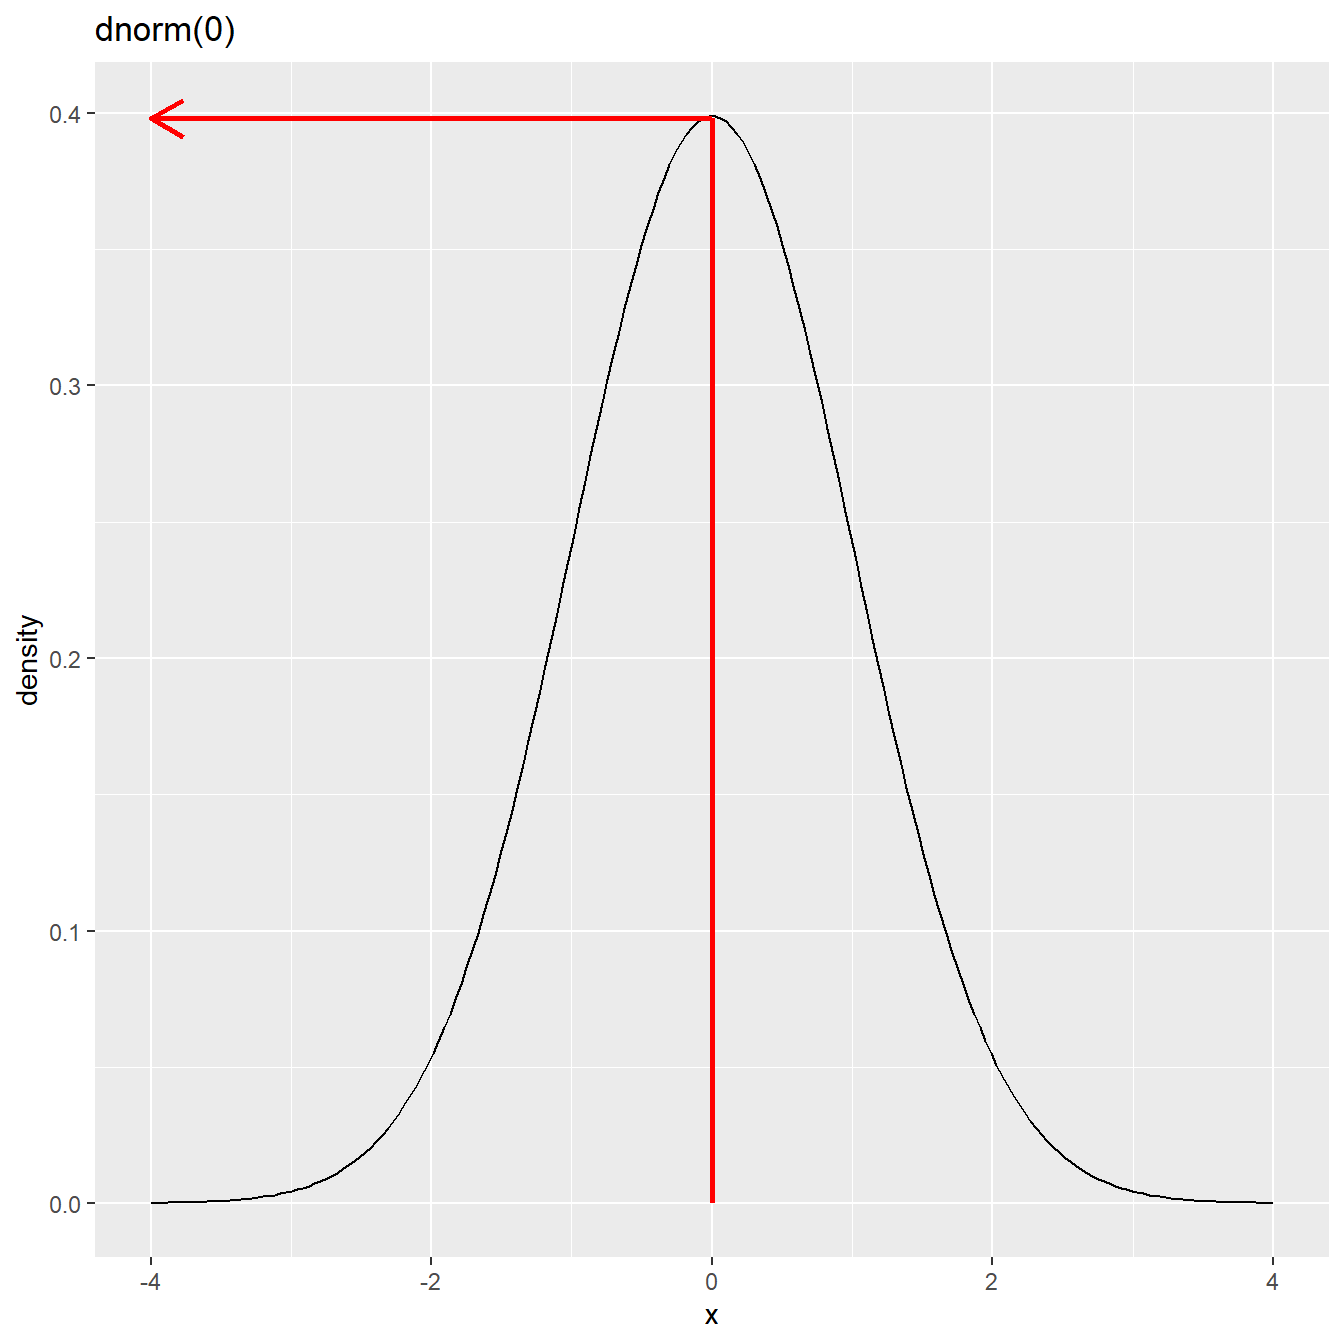
\includegraphics[keepaspectratio]{chap3_files/figure-pdf/unnamed-chunk-14-1.pdf}}

}

\caption{Standard normal probability density function: dnorm(0)}

\end{figure}%

\subsection{pnorm}\label{pnorm}

\begin{Shaded}
\begin{Highlighting}[]
\FunctionTok{pnorm}\NormalTok{(}\DecValTok{0}\NormalTok{)}
\end{Highlighting}
\end{Shaded}

\begin{verbatim}
[1] 0.5
\end{verbatim}

\begin{figure}[H]

{\centering \pandocbounded{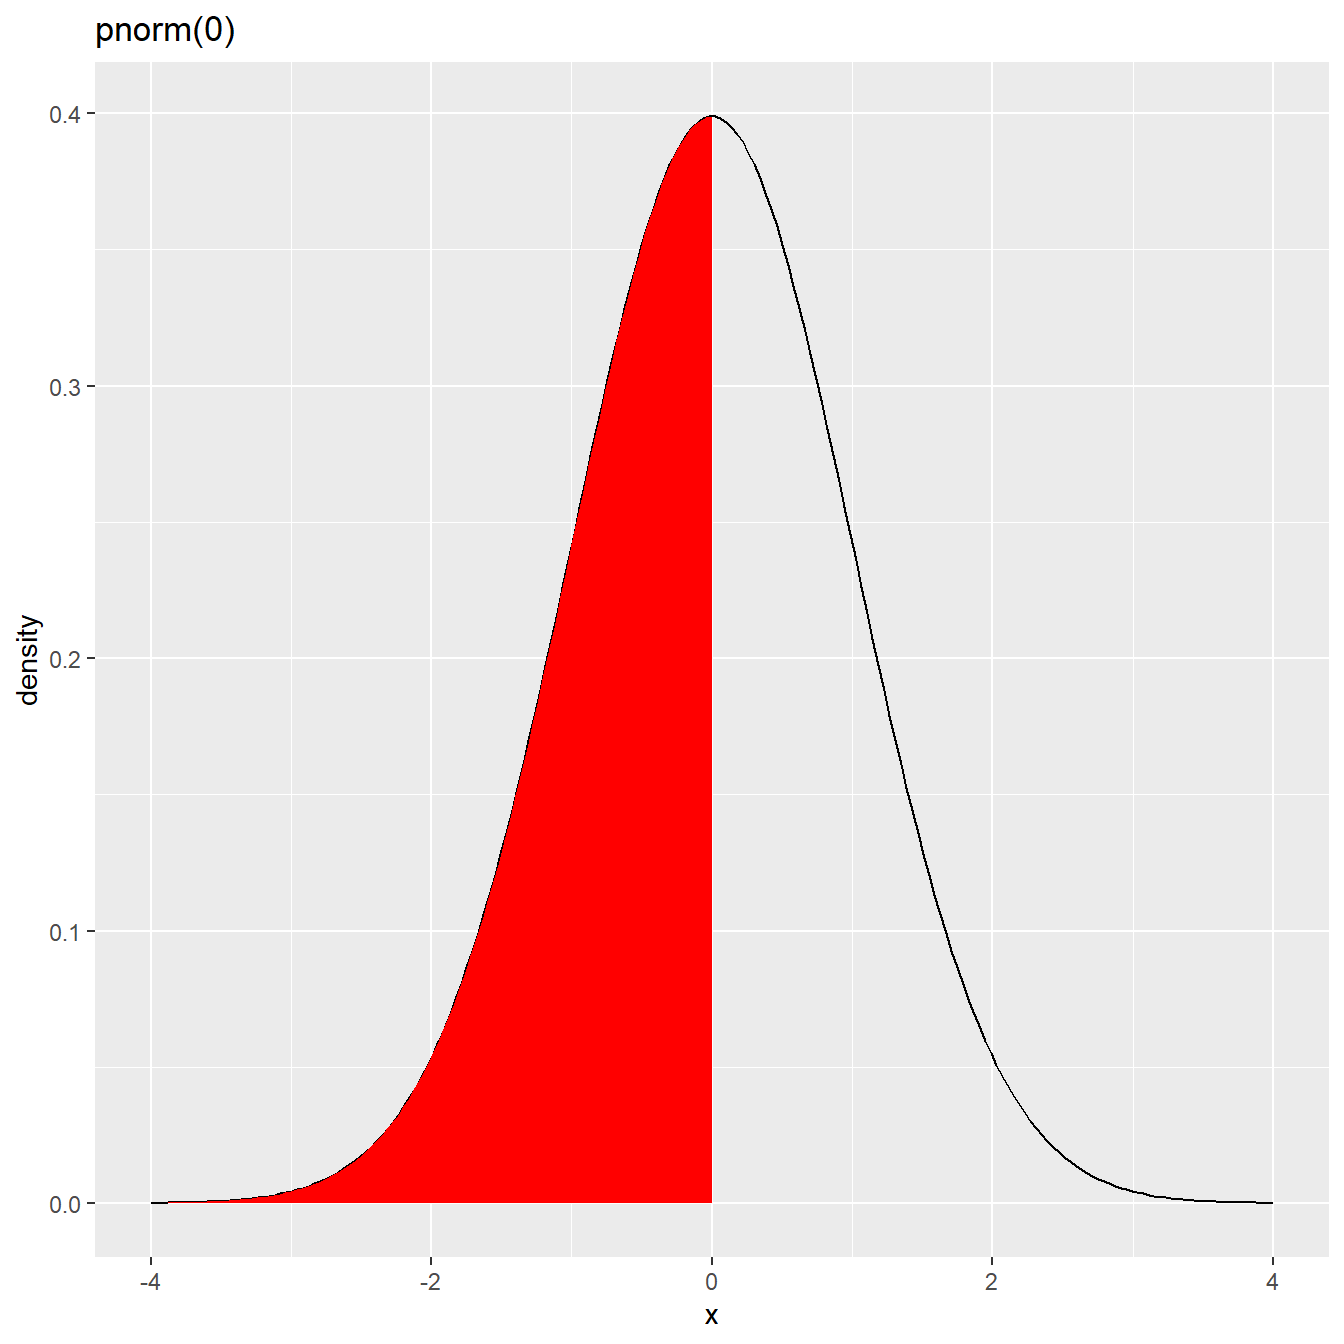
\includegraphics[keepaspectratio]{chap3_files/figure-pdf/unnamed-chunk-16-1.pdf}}

}

\caption{Standard normal probability density function: pnorm(0)}

\end{figure}%

{]}

\subsection{qnorm}\label{qnorm}

\begin{Shaded}
\begin{Highlighting}[]
\FunctionTok{qnorm}\NormalTok{(}\FloatTok{0.5}\NormalTok{)}
\end{Highlighting}
\end{Shaded}

\begin{verbatim}
[1] 0
\end{verbatim}

\begin{figure}[H]

{\centering \pandocbounded{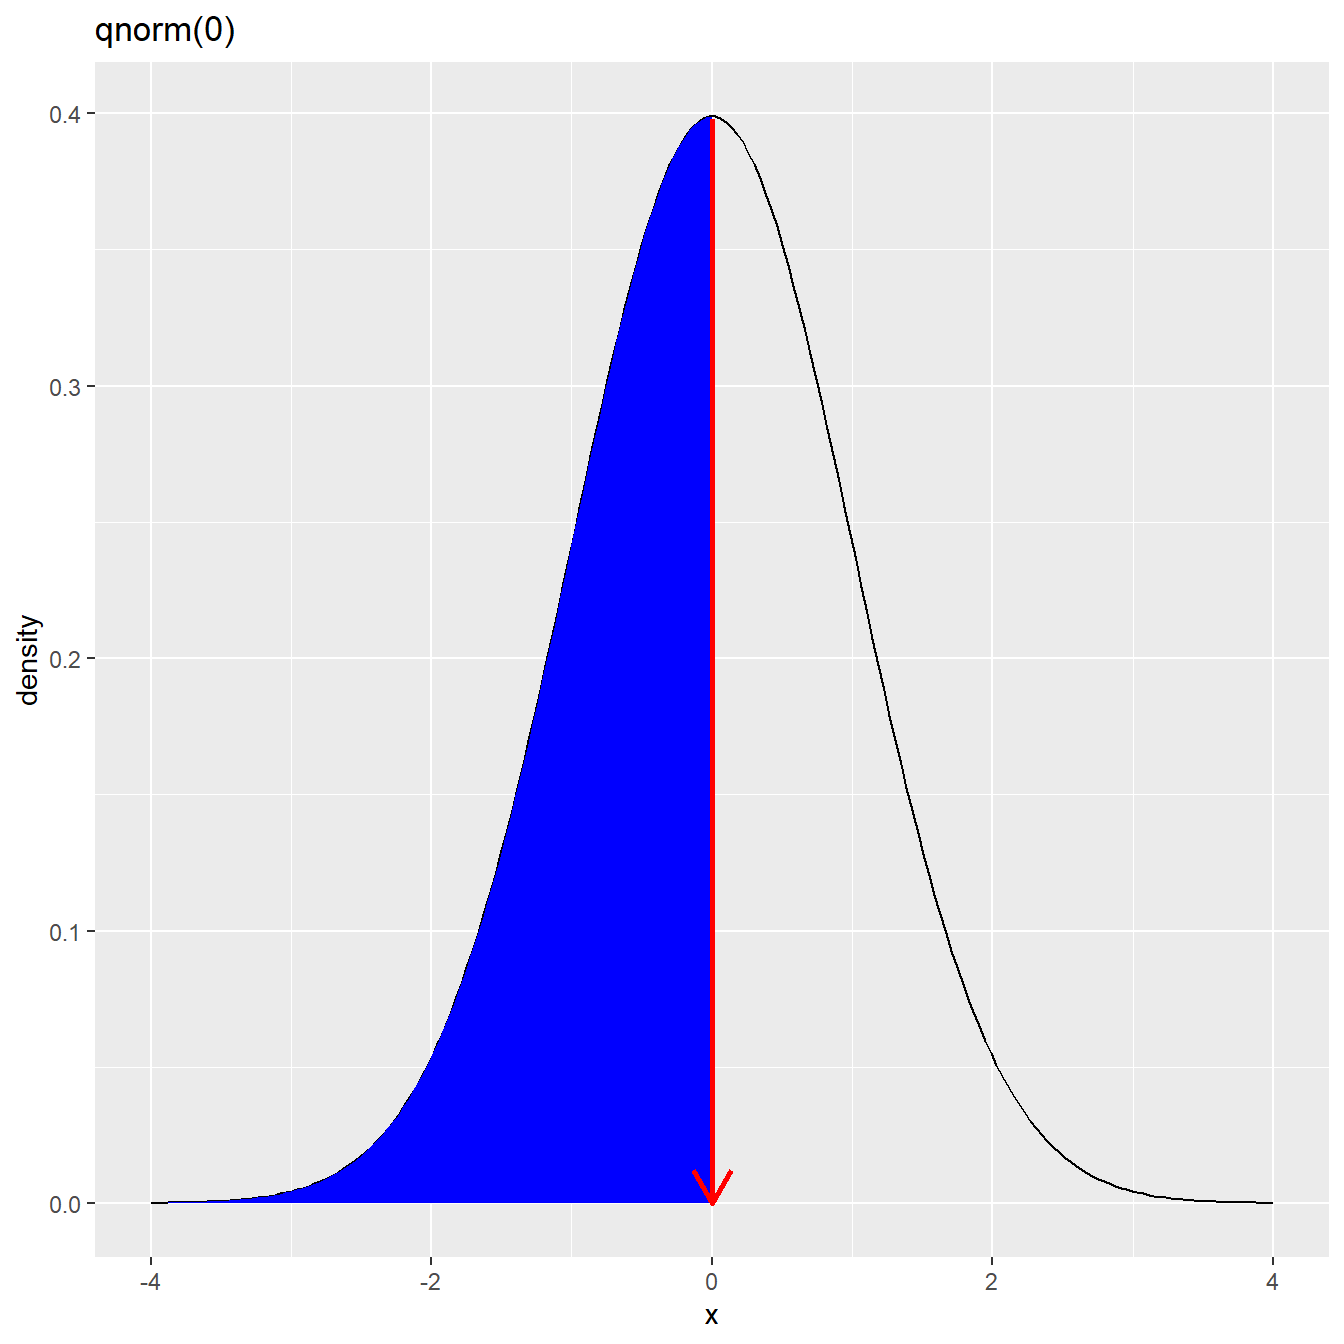
\includegraphics[keepaspectratio]{chap3_files/figure-pdf/unnamed-chunk-18-1.pdf}}

}

\caption{Standard normal probability density function: qnorm(0.5)}

\end{figure}%

\section{Test and Type conversion
functions}\label{test-and-type-conversion-functions}

\begin{longtable}[]{@{}ll@{}}
\toprule\noalign{}
Test & Convert \\
\midrule\noalign{}
\endhead
\bottomrule\noalign{}
\endlastfoot
& \\
is.numeric() & as.numeric() \\
is.character() & as.character() \\
is.vector() & as.vector() \\
is.matrix() & as.matrix() \\
is.data.frame() & as.data.frame() \\
is.factor() & as.factor() \\
is.logical() & as.logical() \\
is.na() & \\
\end{longtable}

\bookmarksetup{startatroot}

\chapter{Writing Your Own Functions}\label{writing-your-own-functions}

Sometimes we need to create our own functions for a specific purpose.
They are called user-defined functions.

\section{Syntax}\label{syntax}

👉 Functions are created using the \texttt{function()}

Main components of a function

\begin{itemize}
\item
  Function name
\item
  Function inputs
\item
  Function body
\item
  Function output
\end{itemize}

\begin{Shaded}
\begin{Highlighting}[]

\NormalTok{name }\OtherTok{\textless{}{-}} \ControlFlowTok{function}\NormalTok{(arg1, aug2, ...)\{}

\SpecialCharTok{\textless{}}\NormalTok{FUNCTION BODY}\SpecialCharTok{\textgreater{}}

\FunctionTok{return}\NormalTok{(value)}

\NormalTok{\}}
\end{Highlighting}
\end{Shaded}

\textbf{Example}

\begin{Shaded}
\begin{Highlighting}[]
\NormalTok{cal\_power }\OtherTok{\textless{}{-}} \ControlFlowTok{function}\NormalTok{(x)\{}

\NormalTok{a }\OtherTok{\textless{}{-}}\NormalTok{ x}\SpecialCharTok{\^{}}\DecValTok{2}\NormalTok{; b }\OtherTok{\textless{}{-}}\NormalTok{ x}\SpecialCharTok{\^{}}\DecValTok{3}
\NormalTok{out }\OtherTok{\textless{}{-}} \FunctionTok{c}\NormalTok{(a, b)}
\FunctionTok{names}\NormalTok{(out) }\OtherTok{\textless{}{-}} \FunctionTok{c}\NormalTok{(}\StringTok{"squared"}\NormalTok{, }\StringTok{"cubed"}\NormalTok{)}
\NormalTok{out }\CommentTok{\# or return(out)}

\NormalTok{\}}
\end{Highlighting}
\end{Shaded}

\textbf{Evaluation}

\begin{Shaded}
\begin{Highlighting}[]
\FunctionTok{cal\_power}\NormalTok{(}\DecValTok{2}\NormalTok{)}
\end{Highlighting}
\end{Shaded}

\begin{verbatim}
squared   cubed 
      4       8 
\end{verbatim}

\section{Function with single line}\label{function-with-single-line}

\textbf{Mathod 1}

\begin{Shaded}
\begin{Highlighting}[]
\NormalTok{cal\_sqrt }\OtherTok{\textless{}{-}} \ControlFlowTok{function}\NormalTok{(x)\{}

\NormalTok{x}\SpecialCharTok{\^{}}\DecValTok{2}

\NormalTok{\}}
\end{Highlighting}
\end{Shaded}

\textbf{Method 2}

\begin{Shaded}
\begin{Highlighting}[]
\NormalTok{cal\_sqrt }\OtherTok{\textless{}{-}} \ControlFlowTok{function}\NormalTok{(x) x}\SpecialCharTok{\^{}}\DecValTok{2}
\end{Highlighting}
\end{Shaded}

\section{Exercise}\label{exercise-8}

\begin{enumerate}
\def\labelenumi{\arabic{enumi}.}
\tightlist
\item
  Write a function to calculate the median.
\end{enumerate}

help:

\begin{Shaded}
\begin{Highlighting}[]
\DecValTok{5}\SpecialCharTok{\%\%}\DecValTok{2}
\end{Highlighting}
\end{Shaded}

\begin{verbatim}
[1] 1
\end{verbatim}

\begin{Shaded}
\begin{Highlighting}[]
\DecValTok{4}\SpecialCharTok{\%\%}\DecValTok{2}
\end{Highlighting}
\end{Shaded}

\begin{verbatim}
[1] 0
\end{verbatim}

\begin{enumerate}
\def\labelenumi{\arabic{enumi}.}
\setcounter{enumi}{1}
\tightlist
\item
  Write a function to calculate the correlation coefficient
\end{enumerate}

\[r=\frac{\sum_{i=1}^{n}(x_i-\bar{x})(y_i-\bar{y})}{\sqrt{\sum_{i=1}^n(x_i-\bar{x})^2\sum_{i=1}^n(y_i-\bar{y})^2}}\]

\bookmarksetup{startatroot}

\chapter{Control Structures}\label{control-structures}

\bookmarksetup{startatroot}

\chapter{Introduction to Tidyverse}\label{introduction-to-tidyverse}

\bookmarksetup{startatroot}

\chapter{Data Wrangling}\label{data-wrangling}

\section{Exercise}\label{exercise-9}

This exercise is based on the \texttt{DStidy} dataset from the
\texttt{DSjobtracker} package in R. This dataset was compiled from job
advertisements for roles like statisticians and data scientists. It
includes information on job roles, required qualifications, technical
and soft skills, tools, platforms, and other relevant criteria
frequently mentioned in the job advertisements. Write R code to answer
each question. Use the provided output to verify the correctness of your
code.

\begin{enumerate}
\def\labelenumi{\arabic{enumi}.}
\tightlist
\item
  How many job advertisements mention both \texttt{R} and
  \texttt{Python} as required skills?
\end{enumerate}

\begin{verbatim}
[1] 437
\end{verbatim}

\begin{enumerate}
\def\labelenumi{\arabic{enumi}.}
\setcounter{enumi}{1}
\tightlist
\item
  Which job categories require R but not Python?
\end{enumerate}

Help: \texttt{distinct} function

\begin{verbatim}
# A tibble: 20 x 1
   Job_Category                                   
   <chr>                                          
 1 Unimportant                                    
 2 Data Science                                   
 3 Data Science and Data Engineering              
 4 Data Analyst                                   
 5 <NA>                                           
 6 AI                                             
 7 Business/Systems Analysts                      
 8 Computer/Information Technology                
 9 Science & Technology                           
10 Sciences                                       
11 Statistics                                     
12 Data science                                   
13 Information Services                           
14 Analyst, Engineering and Information Technology
15 Research, Analyst, and Information Technology  
16 Analyst                                        
17 Administrative                                 
18 Machine Learning                               
19 Data Analytics                                 
20 Actuarial Science                              
\end{verbatim}

\begin{enumerate}
\def\labelenumi{\arabic{enumi}.}
\setcounter{enumi}{2}
\tightlist
\item
  What is the most common educational qualification required
  (BSc\_needed, MSc\_needed, PhD\_needed) across all job categories?
\end{enumerate}

\begin{verbatim}
# A tibble: 1 x 3
    BSc   MSc   PhD
  <int> <int> <int>
1   293   152    71
\end{verbatim}

\begin{enumerate}
\def\labelenumi{\arabic{enumi}.}
\setcounter{enumi}{3}
\tightlist
\item
  What is the average salary for job roles that require SQL, grouped by
  Job\_Category?
\end{enumerate}

\begin{verbatim}
# A tibble: 26 x 2
   Job_Category                                  avg_salary
   <chr>                                              <dbl>
 1 Unimportant                                    11108498.
 2 <NA>                                            4689542.
 3 Machine Learning                                 108000 
 4 Data Analyst                                     107890 
 5 Data Science                                     102805.
 6 AI                                                95000 
 7 Data Science and Data Engineering                 78500 
 8 Data science                                      75125.
 9 Research, Analyst, and Information Technology     70970.
10 Internet Publishing                               70000 
# i 16 more rows
\end{verbatim}

\begin{enumerate}
\def\labelenumi{\arabic{enumi}.}
\setcounter{enumi}{4}
\tightlist
\item
  Calculate the proportion of job advertisements that require English by
  City.
\end{enumerate}

\begin{verbatim}
# A tibble: 299 x 2
   City            Prop_English
   <chr>                  <dbl>
 1 Anaheim                    1
 2 Arges                      1
 3 Athens                     1
 4 Attiki                     1
 5 Berlin                     1
 6 Bugis                      1
 7 Calgary                    1
 8 Central Denmark            1
 9 Chengdu                    1
10 Darmstadt                  1
# i 289 more rows
\end{verbatim}

\begin{enumerate}
\def\labelenumi{\arabic{enumi}.}
\setcounter{enumi}{5}
\tightlist
\item
  Select only the columns: ID, Job\_title, Company, and City.
\end{enumerate}

\begin{verbatim}
# A tibble: 1,172 x 4
      ID Job_title                                   Company               City 
   <dbl> <chr>                                       <chr>                 <chr>
 1     1 <NA>                                        <NA>                  <NA> 
 2     2 Junior Data Scientist                       Dialog Axiata PLC     Colo~
 3     3 Engineer, Analytics & Data Science          London Stock Exchang~ Colo~
 4     4 CI-Statistical Analyst/Business Analyst-CMB E.D. Bullard Company  Colo~
 5     5 DA-Data Analyst-CMB                         E.D. Bullard Company  Colo~
 6     6 Data Scientist                              Emirates Center for ~ Kual~
 7     7 Principal HR Data Scientist                 BHP Group Limited     Kual~
 8     8 DV-Data Visualization & QA Specialist-CMB   E.D. Bullard Company  Colo~
 9     9 Product Manager, Product Data Science       Numerator             Otta~
10    10 Associate Director, Data Science            Phreesia Inc.         Otta~
# i 1,162 more rows
\end{verbatim}

\begin{enumerate}
\def\labelenumi{\arabic{enumi}.}
\setcounter{enumi}{6}
\tightlist
\item
  Filter the dataset to include only jobs that mention Python as a
  required skill.
\end{enumerate}

\begin{verbatim}
# A tibble: 774 x 109
      ID Consultant DateRetrieved       DatePublished       Job_title    Company
   <dbl> <chr>      <dttm>              <dttm>              <chr>        <chr>  
 1     1 Thiyanga   2020-08-05 00:00:00 NA                  <NA>         <NA>   
 2     2 Jayani     2020-08-07 00:00:00 2020-07-31 00:00:00 Junior Data~ Dialog~
 3     3 Jayani     2020-08-07 00:00:00 2020-08-06 00:00:00 Engineer, A~ London~
 4     6 Jayani     2020-08-07 00:00:00 2020-08-13 00:00:00 Data Scient~ Emirat~
 5     7 Jayani     2020-08-13 00:00:00 2020-08-13 00:00:00 Principal H~ BHP Gr~
 6    10 Jayani     2020-08-12 00:00:00 2020-08-11 00:00:00 Associate D~ Phrees~
 7    13 Jayani     2020-08-13 00:00:00 2020-08-13 00:00:00 Data Scient~ Visier~
 8    17 Jayani     2020-08-13 00:00:00 2020-08-11 00:00:00 Data Scienc~ Clearb~
 9    18 Jayani     2020-08-13 00:00:00 2020-08-12 00:00:00 Marketing i~ Yellow~
10    20 Jayani     2020-08-13 00:00:00 2020-08-13 00:00:00 Data Analyst Ernst ~
# i 764 more rows
# i 103 more variables: R <dbl>, SAS <dbl>, SPSS <dbl>, Python <dbl>,
#   MAtlab <dbl>, Scala <dbl>, `C#` <dbl>, `MS Word` <dbl>, `Ms Excel` <dbl>,
#   `OLE/DB` <dbl>, `Ms Access` <dbl>, `Ms PowerPoint` <dbl>,
#   Spreadsheets <dbl>, Data_visualization <dbl>, Presentation_Skills <dbl>,
#   Communication <dbl>, BigData <dbl>, Data_warehouse <dbl>,
#   cloud_storage <dbl>, Google_Cloud <dbl>, AWS <dbl>, ...
\end{verbatim}

\begin{enumerate}
\def\labelenumi{\arabic{enumi}.}
\setcounter{enumi}{7}
\tightlist
\item
  Select all columns related to Microsoft Office tools.
\end{enumerate}

\begin{verbatim}
# A tibble: 1,172 x 4
   `MS Word` `Ms Excel` `Ms Access` `Ms PowerPoint`
       <dbl>      <dbl>       <dbl>           <dbl>
 1         0          0           0               0
 2         0          0           0               0
 3         0          0           0               0
 4         0          0           0               0
 5         1          1           1               1
 6         0          0           0               0
 7         0          0           0               0
 8         1          1           0               1
 9         0          0           0               0
10         0          0           0               0
# i 1,162 more rows
\end{verbatim}

\begin{enumerate}
\def\labelenumi{\arabic{enumi}.}
\setcounter{enumi}{8}
\tightlist
\item
  Filter jobs that were published in or after the year 2023.
\end{enumerate}

Help: use \texttt{year} function in the lubridate package

\begin{verbatim}
# A tibble: 251 x 109
      ID Consultant DateRetrieved       DatePublished       Job_title    Company
   <dbl> <chr>      <dttm>              <dttm>              <chr>        <chr>  
 1     1 Kavya      2023-01-05 18:30:00 2023-01-04 18:30:00 Senior Engi~ DFCC B~
 2     2 Kavya      2023-01-05 18:30:00 2023-01-04 18:30:00 Database En~ <NA>   
 3     3 Kavya      2023-01-05 18:30:00 2023-01-03 18:30:00 Database Ad~ Abans  
 4     4 Kavya      2023-01-05 18:30:00 2023-01-02 18:30:00 Consulting ~ George~
 5     6 Kavya      2023-01-05 18:30:00 2023-01-05 18:30:00 Data Scient~ LSEG   
 6     7 Kavya      2023-01-05 18:30:00 2023-01-05 18:30:00 D & A Azure~ Ernst ~
 7     8 Kavya      2023-01-05 18:30:00 2023-01-04 18:30:00 Data Analyst Novels~
 8     9 Kavya      2023-01-05 18:30:00 2023-01-04 18:30:00 Data Analyst ADA    
 9    10 Kavya      2023-01-05 18:30:00 2023-01-04 18:30:00 Machine Lea~ Bestka~
10    12 Kavya      2023-01-05 18:30:00 2023-01-05 18:30:00 Data Scient~ JKH    
# i 241 more rows
# i 103 more variables: R <dbl>, SAS <dbl>, SPSS <dbl>, Python <dbl>,
#   MAtlab <dbl>, Scala <dbl>, `C#` <dbl>, `MS Word` <dbl>, `Ms Excel` <dbl>,
#   `OLE/DB` <dbl>, `Ms Access` <dbl>, `Ms PowerPoint` <dbl>,
#   Spreadsheets <dbl>, Data_visualization <dbl>, Presentation_Skills <dbl>,
#   Communication <dbl>, BigData <dbl>, Data_warehouse <dbl>,
#   cloud_storage <dbl>, Google_Cloud <dbl>, AWS <dbl>, ...
\end{verbatim}

\begin{enumerate}
\def\labelenumi{\arabic{enumi}.}
\setcounter{enumi}{9}
\tightlist
\item
  Filter the jobs where both PhD\_needed and MSc\_needed are 0.
\end{enumerate}

\begin{verbatim}
# A tibble: 758 x 109
      ID Consultant DateRetrieved       DatePublished       Job_title    Company
   <dbl> <chr>      <dttm>              <dttm>              <chr>        <chr>  
 1     1 Thiyanga   2020-08-05 00:00:00 NA                  <NA>         <NA>   
 2     2 Jayani     2020-08-07 00:00:00 2020-07-31 00:00:00 Junior Data~ Dialog~
 3     3 Jayani     2020-08-07 00:00:00 2020-08-06 00:00:00 Engineer, A~ London~
 4     4 Jayani     2020-08-07 00:00:00 2020-07-24 00:00:00 CI-Statisti~ E.D. B~
 5     5 Jayani     2020-08-07 00:00:00 2020-07-24 00:00:00 DA-Data Ana~ E.D. B~
 6     7 Jayani     2020-08-13 00:00:00 2020-08-13 00:00:00 Principal H~ BHP Gr~
 7     8 Jayani     2020-08-07 00:00:00 2020-07-24 00:00:00 DV-Data Vis~ E.D. B~
 8     9 Jayani     2020-08-13 00:00:00 2020-08-13 00:00:00 Product Man~ Numera~
 9    10 Jayani     2020-08-12 00:00:00 2020-08-11 00:00:00 Associate D~ Phrees~
10    11 Jayani     2020-08-13 00:00:00 2020-08-13 00:00:00 Data Engine~ SDK    
# i 748 more rows
# i 103 more variables: R <dbl>, SAS <dbl>, SPSS <dbl>, Python <dbl>,
#   MAtlab <dbl>, Scala <dbl>, `C#` <dbl>, `MS Word` <dbl>, `Ms Excel` <dbl>,
#   `OLE/DB` <dbl>, `Ms Access` <dbl>, `Ms PowerPoint` <dbl>,
#   Spreadsheets <dbl>, Data_visualization <dbl>, Presentation_Skills <dbl>,
#   Communication <dbl>, BigData <dbl>, Data_warehouse <dbl>,
#   cloud_storage <dbl>, Google_Cloud <dbl>, AWS <dbl>, ...
\end{verbatim}

\begin{enumerate}
\def\labelenumi{\arabic{enumi}.}
\setcounter{enumi}{10}
\tightlist
\item
  Filter out all rows where Salary is missing (NA).
\end{enumerate}

\begin{verbatim}
# A tibble: 239 x 109
      ID Consultant DateRetrieved       DatePublished       Job_title    Company
   <dbl> <chr>      <dttm>              <dttm>              <chr>        <chr>  
 1    12 Jayani     2020-08-13 00:00:00 2020-08-13 00:00:00 Data Analyst EPCOR ~
 2    24 Jayani     2020-08-13 00:00:00 2020-08-13 00:00:00 Data Scient~ Elabra~
 3    45 Jayani     2020-08-13 00:00:00 2020-08-11 00:00:00 Associate P~ SnapHu~
 4    52 Thimani    2020-08-07 00:00:00 2020-07-24 00:00:00 Data Scienc~ Summit~
 5    54 Thimani    2020-08-07 00:00:00 2020-08-01 00:00:00 Data Scient~ PA con~
 6    56 Thimani    2020-08-07 00:00:00 2020-07-31 00:00:00 Data Scient~ Brilli~
 7    57 Thimani    2020-08-07 00:00:00 2020-07-14 00:00:00 Data Scient~ G-Rese~
 8    58 Thimani    2020-08-07 00:00:00 2020-07-19 00:00:00 Manager-Dat~ Biz2Cr~
 9    62 Thimani    2020-08-09 00:00:00 2020-07-19 00:00:00 Senior Mana~ Britis~
10    63 Thimani    2020-08-09 00:00:00 2020-07-23 00:00:00 VP, Data Sc~ 7Park ~
# i 229 more rows
# i 103 more variables: R <dbl>, SAS <dbl>, SPSS <dbl>, Python <dbl>,
#   MAtlab <dbl>, Scala <dbl>, `C#` <dbl>, `MS Word` <dbl>, `Ms Excel` <dbl>,
#   `OLE/DB` <dbl>, `Ms Access` <dbl>, `Ms PowerPoint` <dbl>,
#   Spreadsheets <dbl>, Data_visualization <dbl>, Presentation_Skills <dbl>,
#   Communication <dbl>, BigData <dbl>, Data_warehouse <dbl>,
#   cloud_storage <dbl>, Google_Cloud <dbl>, AWS <dbl>, ...
\end{verbatim}

\begin{enumerate}
\def\labelenumi{\arabic{enumi}.}
\setcounter{enumi}{11}
\tightlist
\item
  For each Experience\_Category, compute the percentage of jobs that
  require Presentation\_Skills.
\end{enumerate}

\begin{verbatim}
# A tibble: 5 x 2
  Experience_Category                prop_presentation
  <chr>                                          <dbl>
1 More than 10 years                             0.25 
2 More than 2 and less than 5 years              0.306
3 More than 5 and less than 10 years             0.318
4 Two or less years                              0.275
5 Unknown or Not needed                          0.360
\end{verbatim}

\bookmarksetup{startatroot}

\chapter{Data Visualisation with Grammar of
Graphics}\label{data-visualisation-with-grammar-of-graphics}

\bookmarksetup{startatroot}

\chapter{Reproducible Documenting with
R}\label{reproducible-documenting-with-r}

\bookmarksetup{startatroot}

\chapter{Regression Analysis}\label{regression-analysis}

\section{Introduction}\label{introduction}

\section{Simple Linear Regression}\label{simple-linear-regression}

\section{Multiple Linear Regression}\label{multiple-linear-regression}

\section{Regression with Dummy
Variables}\label{regression-with-dummy-variables}

\section{Exercise}\label{exercise-10}

\begin{enumerate}
\def\labelenumi{\arabic{enumi}.}
\tightlist
\item
  To understand the effectiveness of marketing investments, a manager of
  a company wants to analyze the relationship between marketing
  expenditures (USD) and the number of sales. Fit a simple linear
  regression model with marketing spend as the independent variable and
  sales as the dependent variable. Interpret the outputs. Note that,
  before fitting a regression model, it is essential to conduct an
  exploratory analysis.
\end{enumerate}

\begin{longtable}[]{@{}cc@{}}
\toprule\noalign{}
Marketing expenditures (USD) & Number of Sales \\
\midrule\noalign{}
\endhead
\bottomrule\noalign{}
\endlastfoot
100 & 522.3 \\
115 & 596.2 \\
120 & 617.7 \\
132 & 682.3 \\
144 & 740.2 \\
154 & 792.5 \\
158 & 806.4 \\
160 & 813.5 \\
170 & 871.0 \\
180 & 920.6 \\
181 & 927.9 \\
190 & 968.5 \\
200 & 1021.6 \\
210 & 1068.2 \\
220 & 1118.9 \\
230 & 1171.2 \\
240 & 1217.3 \\
250 & 1272.1 \\
260 & 1323.6 \\
270 & 1369.6 \\
\end{longtable}

2.To evaluate the association of marketing expenditures on sales, a
company manager aims to analyze the relationship between marketing
expenditures and sales across two different locations. Fit a multiple
linear regression model with marketing expenditures and location as the
independent variables and sales as the dependent variable. Interpret the
outputs. Note that, before fitting a regression model, it is essential
to conduct an exploratory analysis.

\begin{longtable}[]{@{}ccc@{}}
\toprule\noalign{}
Marketing expenditures (USD) & Number of Sales & Location \\
\midrule\noalign{}
\endhead
\bottomrule\noalign{}
\endlastfoot
100 & 522.3 & A \\
115 & 596.2 & A \\
120 & 617.7 & A \\
132 & 682.3 & A \\
144 & 740.2 & A \\
154 & 792.5 & A \\
158 & 806.4 & A \\
160 & 813.5 & A \\
170 & 871.0 & A \\
180 & 920.6 & A \\
181 & 927.9 & A \\
190 & 968.5 & A \\
200 & 1021.6 & A \\
210 & 1068.2 & A \\
220 & 1118.9 & A \\
230 & 1171.2 & A \\
240 & 1217.3 & A \\
250 & 1272.1 & A \\
260 & 1323.6 & A \\
270 & 1369.6 & A \\
100 & 522.3 & B \\
115 & 596.2 & B \\
120 & 617.7 & B \\
132 & 682.3 & B \\
144 & 740.2 & B \\
154 & 792.5 & B \\
158 & 806.4 & B \\
160 & 813.5 & B \\
170 & 871.0 & B \\
180 & 920.6 & B \\
181 & 927.9 & B \\
190 & 968.5 & B \\
200 & 1021.6 & B \\
210 & 1068.2 & B \\
220 & 1118.9 & B \\
230 & 1171.2 & B \\
240 & 1217.3 & B \\
250 & 1272.1 & B \\
260 & 1323.6 & B \\
270 & 1369.6 & B \\
\end{longtable}

\bookmarksetup{startatroot}

\chapter{Summary}\label{summary}

In summary, this book has no content whatsoever.

\begin{Shaded}
\begin{Highlighting}[]
\DecValTok{1} \SpecialCharTok{+} \DecValTok{1}
\end{Highlighting}
\end{Shaded}

\begin{verbatim}
[1] 2
\end{verbatim}

\bookmarksetup{startatroot}

\chapter*{References}\label{references}
\addcontentsline{toc}{chapter}{References}

\markboth{References}{References}

\phantomsection\label{refs}
\begin{CSLReferences}{0}{1}
\end{CSLReferences}




\end{document}
